%make conclusion more of a summary
%fix references to urls instead make citations
%go through material on the Essenes
%get better references
\documentclass[11pt]{article}
\usepackage[utf8]{inputenc}
\usepackage{titlesec}
\usepackage{lipsum}



\titleclass{\subsubsubsection}{straight}[\subsection]

\newcounter{subsubsubsection}[subsubsection]
\renewcommand\thesubsubsubsection{\thesubsubsection.\arabic{subsubsubsection}}
\renewcommand\theparagraph{\thesubsubsubsection.\arabic{paragraph}} % optional; useful if paragraphs are to be numbered

\titleformat{\subsubsubsection}
  {\normalfont\normalsize\bfseries}{\thesubsubsubsection}{1em}{}
\titlespacing*{\subsubsubsection}
{0pt}{3.25ex plus 1ex minus .2ex}{1.5ex plus .2ex}

\makeatletter
\renewcommand\paragraph{\@startsection{paragraph}{5}{\z@}%
  {3.25ex \@plus1ex \@minus.2ex}%
  {-1em}%
  {\normalfont\normalsize\bfseries}}
\renewcommand\subparagraph{\@startsection{subparagraph}{6}{\parindent}%
  {3.25ex \@plus1ex \@minus .2ex}%
  {-1em}%
  {\normalfont\normalsize\bfseries}}
\def\toclevel@subsubsubsection{4}
\def\toclevel@paragraph{5}
\def\toclevel@paragraph{6}
\def\l@subsubsubsection{\@dottedtocline{4}{7em}{4em}}
\def\l@paragraph{\@dottedtocline{5}{10em}{5em}}
\def\l@subparagraph{\@dottedtocline{6}{14em}{6em}}
\makeatother

\setcounter{secnumdepth}{4}
\setcounter{tocdepth}{4}





%\titleformat{\paragraph}
%{\normalfont\normalsize\bfseries}{\theparagraph}{1em}{}
%\titlespacing*{\paragraph}
%{0pt}{3.25ex plus 1ex minus .2ex}{1.5ex plus .2ex}
%http://tex.stackexchange.com/questions/60209/how-to-add-an-extra-level-of-sections-with-headings-below-subsubsection

\usepackage{graphicx}
\graphicspath{ {images/} }


\usepackage{hyperref}

\usepackage{polyglossia}
\setdefaultlanguage{english}
\setotherlanguage{hebrew}
\setotherlanguage[variant=ancient]{greek}
\usepackage{fontspec}
\newfontfamily\greekfont[Script=Greek]{Linux Libertine O}

%use the following on Linux
%\setmainfont{Frank Ruehl CLM}
%\setmonofont{Miriam Mono CLM}
%\setsansfont{Simple CLM}
\setmainfont{Frank Ruehl CLM}
\setmonofont{Miriam Mono CLM}
\setsansfont{Simple CLM}
%use the following on Windows (you don't need \setmonofont and \setsansfont)
%\setmainfont{Arial}

% Use the following if you only want to change the font for Hebrew
%\newfontfamily\hebrewfont[Script=Hebrew]{David CLM}
%\newfontfamily\hebrewfonttt[Script=Hebrew]{Miriam Mono CLM}
%\newfontfamily\hebrewfontsf[Script=Hebrew]{Simple CLM}
\usepackage{datetime2}
%\usepackage[yyyymmdd]{datetime}
%\renewcommand{\dateseparator}{--}


%redo according to chicago style
\title{\textbf{Unless He Gives up All His Possessions} \large \\ A Biblical Argument for Taking Luke 14:33 Literally (rough draft) }
\begin{large}

\end{large}
\author{\textcircled{c} 2017 -- \the\year \ Anonymous \\ GNU Free Documentation License  }
\date{created: 2017--02 -26 \\ last updated: \today{}}
\begin{document}

\maketitle
\tableofcontents 

\noindent \newline Copyright (C)  2017 -- \the\year \  Anonymous. \newline
Permission is granted to copy, distribute and/or modify this document\newline
under the terms of the GNU Free Documentation License, Version 1.3\newline
or any later version published by the Free Software Foundation;\newline
with no Invariant Sections, no Front-Cover Texts, and no Back-Cover Texts.\newline
A copy of the license is included in the section entitled "GNU\newline
Free Documentation License" at the end of this document.
%look up diciples inner teachings in luke (I know John has some but maybe luke has some too)
%add copyright notice to paper
% write down that Jesus was mentored by John the Baptist and this as evidence: https://www.biblicalarchaeology.org/daily/people-cultures-in-the-bible/jesus-historical-jesus/what-did-jesus-really-look-like/?mqsc=E3905583&utm_source=WhatCountsEmail&utm_medium=BHDDaily%20Newsletter&utm_campaign=ZE7A8XZ00
% mention that in two places it says "one thing you lack" 
\section{Introduction}
\subsection{Luke 14:33 Interpretive Context}
As a disclaimer, we are not advocating for followers of Yeshua (Jesus) to quickly join a commune because there are many dangerous communes. However, we do advocate that everyone who is a serious follower start their search for a proper commune. We will argue this by showing evidence for a literal interpretation Luke 14:33 and presenting a simple argument based on the great commission in Matthew 28. Generally, verses should be interpreted literally by default unless an alternative can be shown and the literal interpretation is less viable than it. We will also argue that this command given by Yeshua is binding for all followers of Christ given the proper situation. We will do this by showing the connections between Matthew 13:35-52, Matthew 19:16-20:16, Matthew 6:19-34, Mark 10:21-30, Luke 12:29-34, Luke 14:25-33, Luke 11:37-41, Luke 16:9-31, Luke 18:29-30, Acts 2:44-47 and Acts 4:33-35. We will also argue, that even if the command is figurative, the literal version is still useful as a test to see if those who follow Christ have died to self, see: Luke 9:23-24, Romans 12:1-2, Ephesians 4:22-24, Philippians 3:8, Galatians 5:24-25, 1 Peter 4:1-2, and many others.\cite{death to self verses} 

In practice we will argue that--at the time it was spoken--Luke 14:33 meant to give up everything to Christ and his group of apostles. Later Luke 14:33 meant for believers to give up their possessions to a local church (based on the definition of the "reign of God" and based on examples of it's practice) then that local church would distribute those possessions to those who had need among them and also to other churches. This would ensure that people were supported after they gave away their possession and that something permanent would be accomplished; the church would address the root problems of poverty rather than just doing something temporarily for people. Examples of this practice can be seen in Acts 2:44-47, Acts 4:33-35, and the common purse that Jesus and his followers kept as evidenced by John 12:5-6 and many other verses. The believers then would live in radical community as evidenced by verses such as Matthew 6:33 and Mark 10:30. However, the giving up of all possessions was not to be done right away by everyone. Not everyone is ready or has a proper community to give to. The verses quoted are Young's Literal Translation of the Bible unless otherwise noted. A simple argument that Luke 14:33 is literal using the context of the new testament follows:

\begin{enumerate}
\item The apostles were commanded to give up everything:
\begin{quote}
And Peter began to say to him, `Lo, we left all, and we followed thee.' 
(Mark 10:28)
\end{quote}
\begin{quote}
and he saith to them, `Come ye after me, and I will make you fishers of men,' and they, immediately, having left the nets, did follow him.
(Matthew 4:19-20)
\end{quote}
\begin{quote}
57 And it came to pass, as they are going on in the way, a certain one
said unto him, ‘I will follow thee wherever thou mayest go, sir;’ 58 and Jesus said to him, ‘The foxes have holes, and the fowls of the heaven places of rest, but the Son of Man hath not where he may recline the head.’ 59 And he said unto another, ‘Be following me;’ and he said, ‘Sir, permit me, having gone away, first to bury my father;’ 60 and Jesus said to him, ‘Suffer the dead to bury their own dead, and thou, having gone away, publish the reign of God.’ 61 And another also said, ‘I will follow thee, sir, but first permit me to take leave of those in my house;’ 62 and Jesus said unto him, ‘No one having put his hand on a plough, and looking back, is fit for the reign of God.’ (Luke 9:57-62 YLT)
\end{quote}
This shows they kept a common purse:
\begin{quote}
`Wherefore was not this ointment sold for three hundred denaries, and given to the poor?' and he said this, not because he was caring for the poor, but because he was a thief, and had the bag, and what things were put in he was carrying. (John 12:5-6) 
\end{quote}
\item The disciples of the apostles were also Jesus's disciples:
\begin{quote}
in this shall all know that ye are my disciples, if ye may have love one to another.' (John 13:35) 
\end{quote}
\begin{quote}
When therefore the Lord knew that the Pharisees heard that Jesus more disciples doth make and baptize than John, (though indeed Jesus himself was not baptizing, but his disciples,) (John 4:1-2) 
\end{quote}
\item The apostles were to teach the disciples to observe everything Jesus had commanded them: 
\begin{quote}
And having come near, Jesus spake to them, saying, `Given to me was all authority in heaven and on earth;
having gone, then, disciple all the nations, (baptizing them -- to the name of the Father, and of the Son, and of the Holy Spirit,
teaching them to observe all, whatever I did command you,) and lo, I am with you all the days -- till the full end of the age.' (Matthew 28:18-20)
\end{quote}
\item Therefore all disciples of Christ were commanded to give up everything.\newline 
\end{enumerate}
\subsection{Possible Objections}
The three possible objections we can foresee are that a literal Luke 14:33 would not fit the context of the early Church, that it conflicts with Deuteronomy 13:1-5 or Deuteronomy 4:2, and that it would conflict with other messages in the Bible. We will attempt to answer these objections.

\subsubsection{Does All The Context Fit?}
We will deal with the fact that there are many cases where people were commanded to believe without giving away their possessions. We will explain this through the idea of gradual learning of the commands of Yeshua and the Torah, another example of which is the letter in Acts chapter fifteen which does not constitute a final goal for the believers in the church. In addition, the commitment to give away all possessions must be done out of devotion to God above all else (even mother and father) and well considered before-hand as Luke 14:25-33 implies. 

\subsubsection{Does It Add To or Contradict The Law?}
In light of Deuteronomy 13:1-4 we will show that this command does not contradict the Torah. In a similar way the different laws given for sacrifice in the Torah do not contradict each other but are for different situations. In addition, even though the command to give all things is not in the Torah, we will show that it was foreshadowed. The command instead applies the principles in the Torah to a different situation. Once the situation of Yeshua and his close followers keeping a common purse or the situation in the Church in Acts chapters 2 and 4 existed, Luke 14:33 could be practiced. As for harmony with Deuteronomy 4:2, it says nothing preventing God adding to the Torah. It may be that the commands outside the instructions to Israel in the Pentateuch should never be taken as additions since they are of a different type of command and meant as an expansion or commentary on the Torah and not as the Torah itself.

\subsubsection{Possible Conflicts}
Several verses will be examined that may run contrary to a total surrender of possessions.

\section{Interpreting the Context}

\subsection{Figurative and Literal} \label{the figurative and literal}
We argue that Luke 14:33 should be interpreted literally unless good evidence of the following types can be shown: 
\begin{enumerate}
\item It is shown to cause conflicts with the rest of the Bible. 
\item There aren't similar verses or ideas in the Bible that provide evidence for it's literal practice. 
\item A similar statement is used idiomatically elsewhere. 
\item Lastly it would cause suspicion if there are no examples of it's practice in the Bible or the Biblical culture. However, this would not be decisive.
 \end{enumerate}
 
Literal interpretation is the default way to interpret. However, we will cite Milton Spenser Terry and admit this depends heavily on the interpreter's biases.\cite{mt}
\begin{quote}
55 for my flesh truly is food, and my blood truly is drink; 56 he who is eating my flesh, and is drinking my blood, doth remain in me, and I in him. (John 6:55-56) \end{quote}
For instance John 6:55-56 should not be interpreted literally since 1. it conflicts with other verses about what is not food, 2 there are no similar literal ideas of this in the Bible. Yeshua hints at number two later saying: "63 the spirit it is that is giving life; the flesh doth not profit anything; the sayings that I speak to you are spirit, and they are life;" (John 6:63) 3 A similar command/statement is used idiomatically elsewhere:
\begin{quote}
37 And in the last, the great day of the feast, Jesus stood and cried, saying, `If any one doth thirst, let him come unto me and drink;
38 he who is believing in me, according as the Writing said, Rivers out of his belly shall flow of living water;'
39 and this he said of the Spirit, which those believing in him were about to receive; for not yet was the Holy Spirit, because Jesus was not yet glorified. (John 7:37-39)
\end{quote}
Admittedly number three is especially prone to bias. 4 We can say for sure that there are no examples of people eating Yeshua in the Bible or the surrounding Biblical culture. \newline In contrast Matthew 5:17-18 should be interpreted literally since it does not cause conflicts with the rest of the Bible, there are examples of the literal practice of the law by followers of Yeshua, and there are other ideas in the Bible that support the law being forever:  "17 `Do not suppose that I came to throw down the law or the prophets -- I did not come to throw down, but to fulfill; 18 for, verily I say to you, till that the heaven and the earth may pass away, one iota or one tittle may not pass away from the law, till that all may come to pass." (Matthew 5:17-18) Likewise we argue that Luke 14:33 should be interpreted literally because all four points can be shown positively in it's favor. A quick summary that will be expanded upon later follows: 1 It does not conflict and in fact allows harmonies of sayings that wouldn't otherwise exist: rich young ruler, no one shall leave house or home without receiving one hundred more in this life etc . . . 2 There are many supporting ideas and verses such as in the parable of the steward, the pearl of great price, and the parable of the vineyard, including the fact that the apostles gave up everything and were told to teach everyone to "observe all, whatever [Christ] did command [them]" (Matthew 28:20) 3 We do not see similar statements being used idiomatically elsewhere in the Bible. 4 There are examples of people giving up their possessions in general (the Essenes) and to follow Yeshua: all the disciples, the rich young ruler, and the church in Acts.

\subsection{The Nature of The Command}
The following provides the most closely relevant context to the command to give up all possessions:
\begin{quote}
25 And there were going on with him great multitudes, and having turned, he said unto them,
26 `If any one doth come unto me, and doth not hate his own father, and mother, and wife, and children, and brothers, and sisters, and yet even his own life, he is not able to be my disciple;
27 and whoever doth not bear his cross, and come after me, is not able to be my disciple.
28 `For who of you, willing to build a tower, doth not first, having sat down, count the expense, whether he have the things for completing?
29 lest that he having laid a foundation, and not being able to finish, all who are beholding may begin to mock him,
30 saying -- This man began to build, and was not able to finish.
31 `Or what king going on to engage with another king in war, doth not, having sat down, first consult if he be able with ten thousand to meet him who with twenty thousand is coming against him?
32 and if not so -- he being yet a long way off -- having sent an embassy, he doth ask the things for peace.
33 `So, then, every one of you who doth not take leave of all that he himself hath, is not able to be my disciple. (Luke 14:16-34)
\end{quote}
We can see here that the context switches from valuing following Christ more than anything to making sure you are willing/able to bear the cost of following him and to carefully consider your decision. The command comes after the subject of bearing the cost and is connected by "So, then" i.e: "So, then . . . you who doth not take leave of all . . . is not able to be my disciple." 

We would argue that it's not just the cost that should be considered here but the whether who/what you are following is legitimate, as Yeshua tells us: "for there shall arise false Christs, and false prophets, and they shall give great signs and wonders, so as to lead astray, if possible, also the chosen." (Matthew 24:24) 

We argue that the best fit for the context of Luke 14:33 is to prevent people from becoming tares/darnel in the reign of God since the reign of God is associated with community and sharing:
 \begin{quote}
24 Another simile he set before them, saying: `The reign of the heavens was likened to a man sowing good seed in his field,
25 and, while men are sleeping, his enemy came and sowed darnel in the midst of the wheat, and went away,
26 and when the herb sprang up, and yielded fruit, then appeared also the darnel.
27 `And the servants of the householder, having come near, said to him, Sir, good seed didst thou not sow in thy field? whence then hath it the darnel?
28 And he saith to them, A man, an enemy, did this; and the servants said to him, Wilt thou, then, [that] having gone away we may gather it up?
29 `And he said, No, lest -- gathering up the darnel -- ye root up with it the wheat,
30 suffer both to grow together till the harvest, and in the time of the harvest I will say to the reapers, Gather up first the darnel, and bind it in bundles, to burn it, and the wheat gather up into my storehouse.' (Matthew 13:24-30)
 \end{quote}
In addition the command in Luke 14:33 is with the situation of the apostles following Yeshua and keeping a common purse. If there's not a community that is like that (in our interpretation: righteous and shares all possessions) then the command would not apply. See \ref{situational sacrifices} for more details on situational commands.


\subsection{Reign of God} 
We now must address the misconception of the "reign of heaven" (another phrase for "reign of God" or more commonly translated "kingdom of God") This is not "heaven" as many people think, for example  "20 And having been questioned by the Pharisees, when the reign of God doth come, he answered them, and said, 'The reign of God doth not come with observation; 21 nor shall they say, Lo, here; or lo, there; for lo, the reign of God is within you.'" (Luke 17:21) "Let the little children come to me . . . for of such is the kingdom of God" (Luke 18:16) While the "reign of God/heaven" doesn't appear in the old testament, the "reign of Yahweh" does and it is made up of the people of Israel, see 2 Chronicles 13:7-8 and 1 Chronicles 28:4-5. Just like God saw the need for Israel and created the laws and rituals that held the national community together we think God saw a need for greater community in the new testament and extended the family unit to the local church. This is the reign of heaven. Therefore The reign of heaven is establishing God's reign over and through the people of God, it is Yeshua's movement of people here on earth. \cite{kh} This means the following verses verses have practical application for Yeshua's followers:  Mark 10:21-31, Matthew 6:19-34, Matthew 13:35-52, Matthew 19:16-20:16, Luke 12:29-34, Luke 16:9-31, Luke 18:29-30. 

\subsection{Disciples}
We must also address a misconception of the word "disciple" (\begin{greek}μαθητής\end{greek} which is Strong's number G3101) When Yeshua says in Luke 14:33 "whoever of you does not forsake all that he has cannot be My disciple [G3101]" he is not using \begin{greek}μαθητής\end{greek} to only refer to his inner circle. First it is not only the Apostles who were his disciples: "13 and when it became day, he called near his disciples, [G3101] and having chosen from them twelve, whom also he named apostles," (Luke 6:13) Second his disciples were supposed to emulate Yeshua: "40 A disciple [G3101] is not above his teacher, but every one perfected shall be as his teacher." (Luke 6:40)
This is the same with the disciples his Apostles made, which where supposed to be baptized in Yeshua's name, and were supposed to emulate everything he taught his apostles: 
"18 And having come near, Jesus spake to them, saying, `Given to me was all authority in heaven and on earth;
19 having gone, then, disciple [G3100 from G3101] all the nations, (baptizing them -- to the name of the Father, and of the Son, and of the Holy Spirit,
20 teaching them to observe all, whatever I did command you,) and lo, I am with you all the days -- till the full end of the age.'" (Matthew 28:18-20) All people the Apostles baptized were Christ's disciples, not theirs: "When therefore the Lord knew that the Pharisees heard that Jesus more disciples [G3101] doth make and baptize than John, 2 (though indeed Jesus himself was not baptizing, but his disciples, G3101)" (John 4:1-2) 

Finally, discipleship is based on following Christ which all believers are supposed to do: "31 Jesus, therefore, said unto the Jews who believed in him, `If ye may remain in my word, truly my disciples ye are, and ye shall know the truth," (John 8:31) "By this all will know that you are My disciples, G3101 if you have love for one another." 
(John 13:35)

The following verses also relate to the reign of God even though the term "disciple" is used: Luke 14:26-33, Acts 4:33-35, and Acts 2:44-47. A disciple is a follower of Yeshua, and Yeshua's movement is the reign of God. This is assumed even when he tells a parable that doesn't mention the reign of God:

"7 And he spake a simile unto those called, marking how they were choosing out the first couches, saying unto them, . . . 
15 And one of those reclining with him, having heard these things, said to him, `Happy [is] he who shall eat bread in the reign of God;'" (Luke 14:7-15)
And believing in Christ is associated with the reign of God,\cite{reign of god} for example:
"17 From that time began Jesus to proclaim and to say, `Reform ye, for come nigh hath the reign of the heavens.'" (Matthew 4:17)
"60 and Jesus said to him, `Suffer the dead to bury their own dead, and thou, having gone away, publish the reign of God.'" (Luke 9:60)
"62 and Jesus said unto him, `No one having put his hand on a plough, and looking back, is fit for the reign of God.'" (Luke 9:62)
 
However, some disciples had to wait for the reign of God because it was either not fully manifested until the church in Acts or because Yeshua did not allow everyone who believed be part of his group with the twelve: 
'43 Joseph of Arimathea, an honourable counsellor, who also himself was waiting for the reign of God, came, boldly entered in unto Pilate, and asked the body of Jesus.' (Mark 15:43)

(also see Luke 23:51 and Luke 2:25) As we shall see Yeshua kept a common purse with the twelve apostles and the reign of God verses connect with other verses that have a common theme: radical community in the form of giving up all possessions, all those possessions being distributed by apostles or leaders, and being satisfied with the same reward as others even though others may not be able to do as much work.

We can also see that the reign of God locally administered. Romans 13 refers to church/synagogue leaders according to Mark D. Nanos in his book "The Mystery of Romans." The Jews and Christians shared the synagogues because Christianity was just considered a sect of Judaism early on. Also Eusebius speaks about the martyrdom of James where there were many Jews who believed in Christ and were at the temple to celebrate the Passover. \cite{martyrdom of james} The synagogues could collect taxes and punish transgressions of the law in many parts of the Roman empire.%[FIX] cite a source for this
This may have been the case in Judea too Mark 12:12 (notice it says they feared the "crowd" not the "Romans") also they seemed to originally be trying to kill Yeshua themselves: Luke 4:28-29, John 5:18, Mark 11:18, John 7:1

Romans 13 says ". . .the authorities that exist are appointed by God. 2 Therefore whoever resists the authority resists the ordinance of God. . ." (NKJV) This relates to Matthew 18:18 ". . . whatever you bind on earth will be bound in heaven . . ." (NKJV) and the surrounding verses which talk of the authority of the community and leaders thereof to enforce God's law and forgive transgressions of God's law. This is in stark contrast to the secular authorities which are in fact mentioned in 1 Peter 2:13 "Therefore submit yourselves to every ordinance of man for the Lord’s sake, whether to the king as supreme," (NKJV) or "13 Be subject, then, to every human creation, because of the Lord, whether to a king, as the highest," (YLT) Notice the contrasting language Romans 13 refers to the laws of the authorities as the "ordinance of God" while in 1 Peter 2 it refers to the laws of the authorities as the "ordinance of man." We are not saying that the synagogue/church leaders are perfect just that their laws are considered divinely binding. Thus, the proper response to bad local leaders is to leave the community not to fight against them. Leaving is easily accomplished because the local leaders do not preside over large areas of land like authorities of nations. Hence we see that the reign of God is locally administered.


\section{Setting the Stage for the Church in Acts}

\subsection{Foreshadowing in The Tanahk} \label{foreshadowing in the tanahk}

\begin{quote}
"3 of the stranger thou mayest exact, and that which is thine with thy brother doth thy hand release;
4 only when there is no needy one with thee, for Jehovah doth greatly bless thee in the land which Jehovah thy God is giving to thee -- an inheritance to possess it.
5 `Only, if thou dost diligently hearken to the voice of Jehovah thy God, to observe to do all this command which I am commanding thee to-day,
6 for Jehovah thy God hath blessed thee as He hath spoken to thee; and thou hast lent [to] many nations, and thou hast not borrowed; and thou hast ruled over many nations, and over thee they do not rule." (Deuteronomy 15:3-6)
\end{quote}
There are a couple things we want to observe here: First the charging of interest is not to be done with believers and is even considered an abomination: Ezekiel 18:13 Second, it was possible for them to not have poor people "with [them]" when they obeyed the commandments. It continues:
\begin{quote}
7 `When there is with thee any needy one of one of thy brethren, in one of thy cities, in thy land which Jehovah thy God is giving to thee, thou dost not harden thy heart, nor shut thy hand from thy needy brother;

8 for thou dost certainly open thy hand to him, and dost certainly lend him sufficient for his lack which he lacketh.

9 `Take heed to thee lest there be a word in thy heart -- worthless, saying, Near [is] the seventh year, the year of release; and thine eye is evil against thy needy brother, and thou dost not give to him, and he hath called concerning thee unto Jehovah, and it hath been in thee sin;

10 thou dost certainly give to him, and thy heart is not sad in thy giving to him, for because of this thing doth Jehovah thy God bless thee in all thy works, and in every putting forth of thy hand;
\end{quote}

Here we clearly see that you are obligated to give--maybe not by the legal system itself but by God. (it isn't optional)

"11 because the needy one doth not cease out of the land, therefore I am commanding thee, saying, Thou dost certainly open thy hand to thy brother, to thy poor, and to thy needy one, in thy land." (Deuteronomy 15:11)

At first this seems like a contradiction with Deuteronomy 15:4 however it is speaking of different groups of people, those "with thee" (v. 4) and poor not ceasing from "your land" (v. 11). Therefore the contradiction may be resolved by comparing those "with you" to those "in the land." It is true that there will always be poor in the land but it is totally possible for there to be no poor "among you." For more details see section \ref{a more intimate command} as well as the same idea in section \ref{added versus joined}

Keil and Delitzsch resolve this passage by arguing that it is in the jussive mood saying the meaning in context is: "Thou needest not to remit a debt to foreigners in the seventh year; thou hast only to take care that there is no poor man with or among thee, that thou dost not cause or increase their poverty, by oppressing the brethren who have borrowed of thee." \cite{jussive mood kd} However, we are left with the question of why make a command with a goal that is stated to be impossible at all times? This would seem to be a difficult command and--if it is difficult--it would contradict Deuteronomy 30:
\begin{quote}
11 `For this command which I am commanding thee to-day, it is not too wonderful for thee, nor [is] it far off.
12 It is not in the heavens, -- saying, Who doth go up for us into the heavens, and doth take it for us, and doth cause us to hear it -- that we may do it.
13 And it [is] not beyond the sea, -- saying, Who doth pass over for us beyond the sea, and doth take it for us, and doth cause us to hear it -- that we may do it?
14 For very near unto thee is the word, in thy mouth, and in thy heart -- to do it. (Deuteronomy 30:11-14)
\end{quote}
There are other ways of resolving this verse and it is beyond the scope of this paper to argue against all of them. Nevertheless the reader is encouraged to compare our resolution to others.

The last verse can be summarized quickly. If we are to love our neighbor as ourselves then shouldn't that be reflected in our actions and provisions for them? Given that is the case what is the point of having our own money? If we truly love our neighbor as ourself there's isn't a reason to keep our money separate. There may need to be elders to organize how that money is spent but there isn't a theoretical reason we should withold anything:
"18 `Thou dost not take vengeance, nor watch the sons of thy people; and thou hast had love to thy neighbour as thyself; I [am] Jehovah."
(Leviticus 19:18)

Some similar verses you can see parallels between follow. We are aware that the theme of desiring the reign of God or the words of God more than food is here. However, we also see a push to eventually get away from working for food or seeking after food as inviduals:
\begin{quote}
1 Ho, every thirsty one, come ye to the waters, And he who hath no money, Come ye, buy and eat, yea, come, buy Without money and without price, wine and milk.
2 Why do ye weigh money for that which is not bread? And your labour for that which is not for satiety? Hearken diligently unto me, and eat good, And your soul doth delight itself in fatness.
3 Incline your ear, and come unto me, Hear, and your soul doth live, And I make for you a covenant age-during, The kind acts of David — that are stedfast. (Isaiah 55)
\end{quote}
\begin{quote}
17 And the Spirit and the Bride say, Come; and he who is hearing -- let him say, Come; and he who is thirsting -- let him come; and he who is willing -- let him take the water of life freely. (Revelation 22:17)
\end{quote}
\begin{quote}
26 Jesus answered them and said, `Verily, verily, I say to you, Ye seek me, not because ye saw signs, but because ye did eat of the loaves, and were satisfied;
27 work not for the food that is perishing, but for the food that is remaining to life age-during, which the Son of Man will give to you, for him did the Father seal -- [even] God.' (John 6:26-27)
\end{quote}
\begin{quote}
'Happy those hungering and thirsting for righteousness -- because they shall be filled."
(Matthew 5:6)
\end{quote}

%Reference Equity and the upside-down kingdom:
%"4 And the strength of the king Hath loved judgment, Thou -- Thou hast established uprightness; Judgment and righteousness in Jacob, Thou -- Thou hast done." (Psalm 99:4)

%http://studybible.info/strongs/H4339
%mesharim see G2112 euthus
%mesharim G1343 dikaiosune
%mesharim G2117 euthus

%http://studybible.info/interlinear/psalm%2099:4
%following connect according to biblehub
% Psalm 9:8
%  Psalm 98:9
%Acts 17:31


\subsection{Leaving All To Follow Yeshua} \label{leaving all to follow yeshua}
John prepared the way for Yeshua with this saying:
"11 and he answering saith to them, `He having two coats -- let him impart to him having none, and he having victuals -- in like manner let him do.'" (Luke 3:11) John strengthened the family unit: "17 and he shall go before Him, in the spirit and power of Elijah, to turn hearts of fathers unto children, and disobedient ones to the wisdom of righteous ones, to make ready for the Lord, a people prepared.'" (Luke 1:17) While John strengthened the family unit Yeshua extended it: 
\begin{quote}
"46 And while he was yet speaking to the multitudes, lo, his mother and brethren had stood without, seeking to speak to him, 47 and one said to him, `Lo, thy mother and thy brethren do stand without, seeking to speak to thee.' 48 And he answering said to him who spake to him, `Who is my mother? and who are my brethren?' 49 And having stretched forth his hand toward his disciples, he said, `Lo, my mother and my brethren! 50 for whoever may do the will of my Father who is in the heavens, he is my brother, and sister, and mother.'" (Matthew 12:46-50)
\end{quote}
Hence shouldn't believers at least share things as a family would? And if John prepared the way for Yeshua with that radical saying of the two cloaks and extra food, wouldn't Yeshua's movement be at least as radical, if not more so? 

In addition the people at Qumran at this time were Essenes \cite{John the Baptist and the Qumran Connection} and John the Baptist was an Essene raised in the Qumran community\cite{John the Baptist and the Qumran Connection} and John the Evangelist and the Gospel of John were profoundly influenced by the Essenes: 
\begin{quote}
"It is conceivable, nevertheless, that some Essene influence came to the evangelist through him, since it is probable that he had been a follower of the Baptist. After more than thirty years of work on John and the Dead Sea Scrolls (usually focusing on the Gospel or on one scroll without thinking about the other), I am persuaded that, while nothing can be clearly demonstrated, a scenario is conceivable. "Let me now present what I am convinced is the best explanation for the pervasive, profound Essene influence on the Fourth Gospel." \cite{Exploring the Gospel of John}
\end{quote}
The Essenes were required to give up all their possessions to Join the community. \cite{Essenes common property} This means that there is strong basis for understanding the commands and context of giving up all in the New Testament as literal in light of the Essenes: 
https://www.biblicalarchaeology.org/daily/biblical-artifacts/dead-sea-scrolls/josephus-on-the-essenes/
\begin{quote}
The Jewish War, Book II, Chapter 8
. . .
(8.3)
122 Since [they are] despisers of wealth—their communal stock is astonishing—, one cannot find a person among them who has more in terms of possessions. For by a law, those coming into the school must yield up their funds to the order, with the result that in all [their ranks] neither the humiliation of poverty nor the superiority of wealth is detectable, but the assets of each one have been mixed in together, as if they were brothers, to create one fund for all. 123 They consider olive oil a stain, and should anyone be accidentally smeared with it he scrubs his body, for they make it a point of honor to remain hard and dry, and to wear white always. Hand-elected are the curators of the communal affairs, and indivisible are they, each and every one, [in pursuing] their functions to the advantage of all."

(8.4)

124 No one city is theirs, but they settle amply in each. And for those school-members who arrive from elsewhere, all that the community has is laid out for them in the same way as if they were their own things, and they go in and stay with those they have never even seen before as if they were the most intimate friends. 125 For this reason they make trips without carrying any baggage at all—though armed on account of the bandits. In each city a steward of the order appointed specially for the visitors is designated quartermaster for clothing and the other amenities. 126 Dress and also deportment of body: like children being educated with fear. They replace neither clothes nor footwear until the old set is ripped all over or worn through with age. 127 Among themselves, they neither shop for nor sell anything; but each one, after giving the things that he has to the one in need, takes in exchange anything useful that the other has. And even without this reciprocal giving, the transfer to them [of goods] from whomever they wish is unimpeded.
\end{quote}
\cite{josephus on the essenes}

In addition there is evidence of Essene influence on the New Testament in general: "It seems widely, and wisely, acknowledged that some Essenes became Christians.
The most striking and impressive parallels between the Dead Sea Scrolls and the New Testament documents are in those compositions produced by the second generation of Christians; hence, the influence from the Essenes did not come most powerfully through John the Baptist or Jesus, although (as I have shown) the points of contact here are also impressive".\cite{Exploring the Gospel of John} It is even thought by some scholars that Yeshua celebrated an Essene Passover as "E. Ruckstuhl has suggested that the Beloved Disciple, the Gospel's trustworthy witness (19:35; 21:24), may have been a monk who once lived in the Essene quarter of Jerusalem. He is impressed by how the Qumran calendar helps to explain the time of Jesus' Last Supper, according to John."\cite{Exploring the Gospel of John} According to the then Pope Ratzinger in 2007 "[Jesus] celebrated the Passover with his disciples in accordance with the Qumran calendar, hence, at least one day earlier; he celebrated it without a lamb, like the Qumran community which did not recognize Herod's temple and was waiting for the new temple." \cite{HOMILY OF HIS HOLINESS BENEDICT XVI} The Essenes were a separatist sect that viewed the priestly system in the temple to be illegitimate. This separatism may explain the Johannine Literature's and maybe other New Testament references to "the Jews." The references make "the Jews" out to be different than the Jewish Apostles and the Jewish Yeshua.
In Paul's usage of the term "works of the law" we know Paul is jousting with an Essene teaching that certain works of the law can make you righteous before God.\cite{Paul MMT} However, the Essene teaching of giving up all possessions is never contradicted, so we can see how the New Testament, and especially John the Baptist--who prepared the way for Yeshau--were influenced by radical ideas. 

\begin{quote}
"43 And fear came on every soul, many wonders also and signs were being done through the apostles, 44 and all those believing were at the same place, and had all things common,
45 and the possessions and the goods they were selling, and were parting them to all, according as any one had need." (Acts 2:43-45)
\end{quote}

\begin{quote}
"34 for there was not any one among them who did lack, for as many as were possessors of fields, or houses, selling [them], were bringing the prices of the thing sold,
35 and were laying them at the feet of the apostles, and distribution was being made to each according as any one had need." (Acts 4:34-35)
\end{quote}

Acts 2:44 and Acts 4:35 were practiced by Yeshua and the disciples before that, as evidenced by Judas's statement where he assumes that those who sold a possession to give to the poor would first deposit it in the community money box (which he kept track of):
"5 `Wherefore was not this ointment sold for three hundred denaries, and given to the poor?' 6 and he said this, not because he was caring for the poor, but because he was a thief, and had the bag, and what things were put in he was carrying." (John 12:5-6) As we have discussed the term disciple applies to everyone who follows Christ, and disciples are supposed to emulate Yeshua. The disciples "left everything" to follow Yeshua: 
\begin{quote}
"And Peter said, `Lo, we left all, and did follow thee;'"
(Luke 18:28)
\end{quote}
Parallels to Luke 18:28 are in Mark 10:28 and Matthew 19:27.
\begin{quote}
18 And Jesus having seen great multitudes about him, did command to depart to the other side;
19 and a certain scribe having come, said to him, `Teacher, I will follow thee wherever thou mayest go;'
20 and Jesus saith to him, `The foxes have holes, and the birds of the heaven places of rest, but the Son of Man hath not where he may lay the head.'
21 And another of his disciples said to him, `Sir, permit me first to depart and to bury my father;'
22 and Jesus said to him, `Follow me, and suffer the dead to bury their own dead.' (Matthew 8:18-22)\end{quote}
\begin{quote}
57 And it came to pass, as they are going on in the way, a certain one said unto him, `I will follow thee wherever thou mayest go, sir;'
58 and Jesus said to him, `The foxes have holes, and the fowls of the heaven places of rest, but the Son of Man hath not where he may recline the head.'
59 And he said unto another, `Be following me;' and he said, `Sir, permit me, having gone away, first to bury my father;'
60 and Jesus said to him, `Suffer the dead to bury their own dead, and thou, having gone away, publish the reign of God.'
61 And another also said, `I will follow thee, sir, but first permit me to take leave of those in my house;'
62 and Jesus said unto him, `No one having put his hand on a plough, and looking back, is fit for the reign of God.' (Luke 9:57-62)\end{quote}
\begin{quote}
18 And Jesus, walking by the sea of Galilee, saw two brothers, Simon named Peter and Andrew his brother, casting a drag into the sea -- for they were fishers --
19 and he saith to them, `Come ye after me, and I will make you fishers of men,'
20 and they, immediately, having left the nets, did follow him.
21 And having advanced thence, he saw other two brothers, James of Zebedee, and John his brother, in the boat with Zebedee their father, refitting their nets, and he called them,
22 and they, immediately, having left the boat and their father, did follow him.
(Matthew 4:18-22)\end{quote}
 \begin{quote}
8 And Simon Peter having seen, fell down at the knees of Jesus, saying, `Depart from me, because I am a sinful man, O lord;'
9 for astonishment seized him, and all those with him, at the draught of the fishes that they took,
10 and in like manner also James and John, sons of Zebedee, who were partners with Simon; and Jesus said unto Simon, `Fear not, henceforth thou shalt be catching men;'
11 and they, having brought the boats upon the land, having left all, did follow him. (Luke 5:8-11)\end{quote}
\begin{quote}
14 And after the delivering up of John, Jesus came to Galilee, proclaiming the good news of the reign of God,
15 and saying -- `Fulfilled hath been the time, and the reign of God hath come nigh, reform ye, and believe in the good news.'
16 And, walking by the sea of Galilee, he saw Simon, and Andrew his brother, casting a drag into the sea, for they were fishers,
17 and Jesus said to them, `Come ye after me, and I shall make you to become fishers of men;' (Mark 1:14-18)\end{quote}
\begin{quote}
27 And after these things he went forth, and beheld a tax-gatherer, by name Levi, sitting at the tax-office, and said to him, `Be following me;'
28 and he, having left all, having arisen, did follow him.
(Luke 5:27-28)\end{quote}

This is not surprising. If we are to give up our life completely and be ready to die, then all our possession are not a big deal:

\begin{quote}
`Because of this I say to you, be not anxious for your life, what ye may eat, and what ye may drink, nor for your body, what ye may put on. Is not the life more than the nourishment, and the body than the clothing? (Matthew 6:25)
27 and whoever doth not bear his cross, and come after me, is not able to be my disciple. (Luke 14:27)
 `He who found his life shall lose it, and he who lost his life for my sake shall find it. (Matthew 10:39) \end{quote}
The change to a centralization of funds reminds of the Old Testament centralization of sacrifices (although that was done on a national scale not locally) see section \ref{situational sacrifices} 

\subsection{Equity, and the Upside-Down Reign}
Once a disciple gives up his possessions as instructed by Luke 14:33 the disciple could not be destitute--as Matthew 6:33 says "but seek ye first the reign of God and His righteousness, and all these shall be added to you." Most people do not read this together with the verses before which say: "31 therefore ye may not be anxious, saying, What may we eat? or, What may we drink? or, What may we put round? 32 for all these do the nations seek for, for your heavenly Father doth know that ye have need of all these;" (Matthew 6) Matthew 6:33 paraphrased is "seek first the reign of God and you won't have to worry about food and drink (basic needs) because they will be provided by your community (reign of God)" In addition to this it says 
\begin{quote}
"29 and every one who left houses, or brothers, or sisters, or father, or mother, or wife, or children, or fields, for my name's sake, an hundredfold shall receive, and life age-during shall inherit; 30 and many first shall be last, and last first. 20:1 `For the reign of the heavens is like to a man, a householder, who went forth with the morning to hire workmen for his vineyard . . ." (Matthew 19:29-20:1)
\end{quote}
The parallels in Luke 18:29-30 and Mark 10:29-30 makes it clear that this receiving a hundredfold will happen in this life: ". . . receive an hundredfold now in this time, houses, and brothers, and sisters, and mothers, and children, and fields, with persecution . . ." (Mark 10:30 YLT) This means total sharing of houses and living in a radical community where everyone is your brother sister or mother. This community is directly connected with the parable of the vineyard where everyone was paid the same. Most people fail to notice that in the parallel of Matthew 6--Luke 12--the lack of worry is connected to the selling of possessions:
\begin{quote}
31 but, seek ye the reign of God, and all these things shall be added to you.
32 `Fear not, little flock, because your Father did delight to give you the reign;
33 sell your goods, and give alms, make to yourselves bags that become not old, a treasure unfailing in the heavens, where thief doth not come near, nor moth destroy;
34 for where your treasure is, there also your heart will be. (Luke 12:31-24)
\end{quote}
Later in the new testament the poor are referred to as those being in the Church:
"(10) The poor—i.e., at Jerusalem and in Judaea. St. Paul had already been the means of bringing contributions from the wealthier churches of Antioch to Jerusalem (Acts 11:29-30). . ." \cite{the poor} This solves the problem of how does one sell everything he has and give to the poor without simply creating himself as a new poor person: he's taken care of by others that keep everything in common. This may fit with the equity (translated "uprightness") described in Psalm 99:4. (see Hebrew definition) %[fix]
"And the strength of the king Hath loved judgment, Thou -- Thou hast established uprightness; Judgment and righteousness in Jacob, Thou -- Thou hast done." (Psalm 99:4) 

\indent To continue with the parable of the vineyard, Matthew 20:1-6 talks about an equality of reward for members in the Kingdom of Heaven:
\begin{quote}
1 `For the reign of the heavens is like to a man, a householder, who went forth with the morning to hire workmen for his vineyard, . . . 11 and having received [it], they were murmuring against the householder, saying, 12 that These, the last, wrought one hour, and thou didst make them equal to us, who were bearing the burden of the day -- and the heat. 13 . . . I do no unrighteousness to thee; for a denary didst not thou agree with me? 16 So the last shall be first, and the first last, for many are called, and few chosen.' (Matthew 20:1-16)
\end{quote}
Matthew 13 talks about people joining the reign of heaven going and selling everything they have, hence making everyone equal with the same treasure of the Kingdom:
\begin{quote}
44 `Again, the reign of the heavens is like to treasure hid in the field, which a man having found did hide, and from his joy goeth, and all, as much as he hath, he selleth, and buyeth that field. 45 `Again, the reign of the heavens is like to a man, a merchant, seeking goodly pearls, 46 who having found one pearl of great price, having gone away, hath sold all, as much as he had, and bought it. (Matthew 13:44-46)
\end{quote}
Both the person and the pearl it compares to the Kingdom of Heaven, implying the Kingdom of God is both made up of people seeking spiritual treasure and is a spiritual treasure itself. 
\begin{quote}
37 And in [his] speaking, a certain Pharisee was asking him that he might dine with him, and having gone in, he reclined (at meat),
38 and the Pharisee having seen, did wonder that he did not first baptize himself before the dinner.
39 And the Lord said unto him, `Now do ye, the Pharisees, the outside of the cup and of the plate make clean, but your inward part is full of rapine and wickedness;
40 unthinking! did not He who made the outside also the inside make?
41 But what ye have give ye [as] alms, and, lo, all things are clean to you. (Luke 11)
\end{quote}

\begin{quote}
26 Jesus answered them and said, `Verily, verily, I say to you, Ye seek me, not because ye saw signs, but because ye did eat of the loaves, and were satisfied;
27 work not for the food that is perishing, but for the food that is remaining to life age-during, which the Son of Man will give to you, for him did the Father seal -- [even] God.'
28 They said therefore unto him, `What may we do that we may work the works of God?'
29 Jesus answered and said to them, `This is the work of God, that ye may believe in him whom He did send.'
30 They said therefore to him, `What sign, then, dost thou, that we may see and may believe thee? what dost thou work?
31 our fathers the manna did eat in the wilderness, according as it is having been written, Bread out of the heaven He gave them to eat.'
32 Jesus, therefore, said to them, `Verily, verily, I say to you, Moses did not give you the bread out of the heaven; but my Father doth give you the true bread out of the heaven;
33 for the bread of God is that which is coming down out of the heaven, and giving life to the world.'
34 They said, therefore, unto him, `Sir, always give us this bread.'
35 And Jesus said to them, `I am the bread of the life; he who is coming unto me may not hunger, and he who is believing in me may not thirst -- at any time;
36 but I said to you, that ye also have seen me, and ye believe not;
37 all that the Father doth give to me will come unto me; and him who is coming unto me, I may in no wise cast without,
38 because I have come down out of the heaven, not that I may do my will, but the will of Him who sent me.
39 `And this is the will of the Father who sent me, that all that He hath given to me I may not lose of it, but may raise it up in the last day;
40 and this is the will of Him who sent me, that every one who is beholding the Son, and is believing in him, may have life age-during, and I will raise him up in the last day.' (John 6:26-40)
\end{quote}

In the above verses Yeshua tells us we shouldn't work for our food. If we don't work for it then how are we to eat? We must be working in a community where we are not working for food. Food should not be on our minds when we work but only the work of God. In John 6:29 and John 6:35 G4100 G1519 is more literally translated as "believe into" according to Thayer's Lexicon: 
\begin{quote}
G1519 \begin{greek} εἰς \end{greek}, a preposition governing the accusative, and denoting entrance into, or direction and limit: into, to, toward, for, among.
\end{quote}

Although this is awkward in English it preserves the idea that by believing they aren't just accepting his existence or even his identity as the messiah but what his identity represents: the life that he lives. They are "believing into him" which is a more intimate type of belief, i.e. his name (which is his character): 
\begin{quote}
“He who believes in Him is not judged; he who does not believe has been judged already, because he has not believed in the name of the [fn]only begotten Son of God. (John 3:18)
\end{quote}
 So when he tells them how to not work for food, he may be telling them to follow his example and live communally:
\begin{quote}
27 work not for the food that is perishing, but for the food that is remaining to life age-during, which the Son of Man will give to you, for him did the Father seal -- [even] God.' 28 They said therefore unto him, `What may we do that we may work the works of God?' 29 Jesus answered and said to them, `This is the work of God, that ye may believe in him whom He did send.' (John 6)
\end{quote}
If we live communally the following verse can be fulfilled with literal food on this earth (although we don't know if he only meant not being hungry and thirsting in a spiritual sense)
\begin{quote}
35 And Jesus said to them, `I am the bread of the life; he who is coming unto me may not hunger, and he who is believing in me may not thirst -- at any time; (John 6)
\end{quote}
Yeshua connects the following parable with the Kingdom of Heaven and possibly a similar idea to the saying "the first shall be last and the last shall be first" this may be referring to the reign of God's fulfillment in the after-life:
\begin{quote}
16 the law and the prophets [are] till John; since then the reign of God is proclaimed good news, and every one doth press into it; . . .
19 `And -- a certain man was rich, and was clothed in purple and fine linen, making merry sumptuously every day,
 . . . 
25 `And Abraham said, Child, remember that thou did receive -- thou -- thy good things in thy life, and Lazarus in like manner the evil things, and now he is comforted, and thou art distressed; (Luke 16) 
\end{quote}
Essentially this upside-down reign has it's finality later but the reign of God is a partial fulfillment of this principle now.

The oft repeated statement: "the first shall be last and the last shall be first" as well as "it is hard for the rich to enter the Kingdom of Heaven" and "woe to the rich" mean that it is harder for rich people to join or function in the reign of God. "Hearken, my brethren beloved, did not God choose the poor of this world, rich in faith, and heirs of the reign that He promised to those loving Him?" (James 2:5) This is because they are more attached to their possessions (maybe because they have worked harder for them or are used to having more than others). This will be shown later from the statement's context in the story of the rich young ruler. This is in no way implying that the rich are evil or less righteous but their handicap arises naturally from their circumstances. After all it is "woe to the rich" not "cursed are the rich."
\begin{quote}
"`But wo to you -- the rich, because ye have got your comfort.
`Wo to you who have been filled -- because ye shall hunger. `Wo to you who are laughing now -- because ye shall mourn and weep.
`Wo to you when all men shall speak well of you -- for according to these things were their fathers doing to false prophets." (Luke 6:24-26)
\end{quote}
\begin{quote}
"`Happy the poor in spirit -- because theirs is the reign of the heavens." (Matthew 5:3) 
\end{quote}
However, even though the rich are not evil, the negative way in which they are spoken of implies a less desirable state of being. Wethink you can take away from this that riches make it more likely for you to commit fraud and get away with it, or become arrogant:
\begin{quote}
"Go, now, ye rich! weep, howling over your miseries that are coming upon [you];
your riches have rotted, and your garments have become moth-eaten;
your gold and silver have rotted, and the rust of them for a testimony shall be to you, and shall eat your flesh as fire. Ye made treasure in the last days!
lo, the reward of the workmen, of those who in-gathered your fields, which hath been fraudulently kept back by you -- doth cry out, and the exclamations of those who did reap into the ears of the Lord of Sabaoth have entered;
ye did live in luxury upon the earth, and were wanton; ye did nourish your hearts, as in a day of slaughter;
ye did condemn -- ye did murder the righteous one, he doth not resist you.
Be patient, then, brethren, till the presence of the Lord; lo, the husbandman doth expect the precious fruit of the earth, being patient for it, till he may receive rain -- early and latter;
be patient, ye also; establish your hearts, because the presence of the Lord hath drawn nigh;" (James 5:1-8)
\end{quote}
As it even says in Proverbs before the declarations of sharing made by Yeshua and John the Baptist: "Vanity and a lying word put far from me, Poverty or wealth give not to me, Cause me to eat the bread of my portion," (Proverbs 30:8)
How do you have neither poverty nor riches for all in a society unless people become equal voluntarily? (forced equality is immoral and ineffectual) These concepts create a reign that truly turns things upside-down:
\begin{quote}
"But the Jews were jealous, and taking some wicked men of the rabble, they formed a mob, set the city in an uproar, and attacked the house of Jason, seeking to bring them out to the crowd. And when they could not find them, they dragged Jason and some of the brothers before the city authorities, shouting, “These men who have  \textbf{turned the world upside down} have come here also," (Acts 17:6 English Standard Version)
\end{quote}
\subsection{No One Can Serve Two Masters}
Most people read Luke 16:8-13 and Matthew 6:19-24 as generalities where believers are supposed to manage their wealth to be useful for God. However, these verses read straightforwardly are radical statements: you cannot store any wealth for yourself and serve God:
\begin{quote} "19 `Treasure not up to yourselves treasures on the earth, where moth and rust disfigure, and where thieves break through and steal, 20 but treasure up to yourselves treasures in heaven, where neither moth nor rust doth disfigure, and where thieves do not break through nor steal, 21 for where your treasure is, there will be also your heart." (Matthew 6:19-21)
\end{quote}
This implies all treasure must be given to, or for the sake of, the Reign of God (i.e. the community of believers) 
The "unrighteous" steward steals from the master because Yeshua is saying that all earthly wealth that isn't given to the community is unrighteous and stealing from God:  
\begin{quote}
"8 ‘And the lord commended the unrighteous steward that he did prudently, because the sons of this age are more prudent than the sons of the light, in respect to their generation." (Luke 16:8)
\end{quote}
In the following it refers to the people in the reign of God as "friends" with the reference to them being able to receive you into "eternal dwellings" and refers to earthly wealth as the "wealth of unrighteousness." "and I say to you, Make to yourselves friends out of the mammon of unrighteousness, that when ye may fail, they may receive you to the age-during tabernacles." (Luke 16:9) In addition the following seems to imply that is not possible to hold any treasure back for oneself: "`He who is faithful in the least, [is] also faithful in much; and he who in the least [is] unrighteous, is also unrighteous in much;" (Luke 16:10) It again calls earthly wealth unrighteous: "if, then, in the unrighteous mammon ye became not faithful -- the true who will entrust to you?" (Luke 16:11) This to us implies that if you do not give up your monetary wealth for God you will not be trusted with true riches. "and if in the other's ye became not faithful -- your own, who shall give to you?" (Luke 16:12) This is referring to wealth really being the possession of God as it says in Job: "Who hath brought before Me and I repay? Under the whole heavens it [is] mine." (Job 41:11) (also see Deuteronomy 10:14 and Haggai 2:8) "your own, who shall give to you?" refers to the reign of God which he gives to us and the true treasure which is spiritual not physical: "32 `Fear not, little flock, because your Father did delight to give you the reign; 33 sell your goods, and give alms, make to yourselves bags that become not old, a treasure unfailing in the heavens, where thief doth not come near, nor moth destroy;" (Luke 12:32-33) also Yeshua said to the rich young ruler in two of three accounts (Mark 10 and Luke 18) "one thing you lack" so go and sell all you have. Also see section \ref{what you truly own} 

The context of these verses is also clear:
\begin{quote}
"`None is able to serve two lords, for either he will hate the one and love the other, or he will hold to the one, and despise the other; ye are not able to serve God and Mammon." (Matthew 6:24)
"`No domestic is able to serve two lords, for either the one he will hate, and the other he will love; or one he will hold to, and of the other he will be heedless; ye are not able to serve God and mammon.'" (Luke 16:13)
\end{quote}
It continues with the theme of wealth and calls it an abomination:
\begin{quote}
"14 And also the Pharisees, being lovers of money, were hearing all these things, and were deriding him, 15 and he said to them, `Ye are those declaring yourselves righteous before men, but God doth know your hearts; because that which among men is high, [is] abomination before God;" (Luke 16:14-15)
\end{quote}
It then connects this teaching to the radical community of the reign of God:
\begin{quote}
"the law and the prophets [are] till John; since then the reign of God is proclaimed good news, and every one doth press into it;" (Luke 16:16)
\end{quote}
In Luke 16 Yeshua then tells a parable of a rich man who did not give to a beggar and in Matthew 6:35-34 it continues with the famous parable of seeking first the reign of God and you will not have to worry about your basic needs, making the context even more clear. 

\subsection{The Rich Young Ruler}
Some people say that the command given to the rich young ruler is for a case like his. Others say it is to be taken literally and applies to everyone. We think both are somewhat correct. Yeshua's exhortation seems to be taking the ruler's statements of keeping the commandments at face value: ". . . ‘One thing thou dost lack; go away, whatever thou hast — sell, and give to the poor, and thou shalt have treasure in heaven, and come, be following me, having taken up the cross.’" (Mark 10:21) Yeshua invites him into the inner circle showing that Yeshua has a positive appreciation for the ruler here. The word translated "ruler" is actually used to refer to the leaders in the synagogue suggestion this man was well known in religious circles and respected. Keeping the commandments just means to guard the commandments \cite{keep meaning} and is completely possible (see Deuteronomy 30:11-14 and Paul's quotation in Romans 10:5-8) 
%also explain psalm 53 quoted in Romans 3:10 and the fact that it says
%all our righteousness is filthy rags, NOTE: MAKE THIS PART OF APPENDIX [fix]
 Notice also Christ seems to associate taking up the cross with these commands.

Yet it is not for everyone to immediately sell their possessions. As it says in Luke 14:25-33 to first consider the cost of your endeavor and make sure your heart is in the right place to follow through with it; this is possibly so one does not become a tare, or a lukewarm participant which is already planted in the reign of God before you are ready. This would cause problems for those who are sincere and probably be worse than not joining at all. However, the rich young ruler had already kept the commandments so Yeshua was giving him the next step if he was ready for it:

"26 `If any one doth come unto me, and doth not hate his own father, and mother, and wife, and children, and brothers, and sisters, and yet even his own life, he is not able to be my disciple;
27 and whoever doth not bear his cross, and come after me, is not able to be my disciple.
28 `For who of you, willing to build a tower, doth not first, having sat down, count the expense, whether he have the things for completing?
29 lest that he having laid a foundation, and not being able to finish, all who are beholding may begin to mock him,
30 saying -- This man began to build, and was not able to finish.
31 `Or what king going on to engage with another king in war, doth not, having sat down, first consult if he be able with ten thousand to meet him who with twenty thousand is coming against him?
32 and if not so -- he being yet a long way off -- having sent an embassy, he doth ask the things for peace.
33 `So, then, every one of you who doth not take leave of all that he himself hath, is not able to be my disciple." (Luke 14:26-33)
The following statements in the story of the rich young ruler imply the context of giving up your things to follow Yeshua was literal:
"28 Then Peter said, "See, we have left all and followed You."" (Luke 18:28)
"28 Then Peter began to say to Him, "See, we have left all and followed You."" (Mark 10:28)

"Then Peter answering said to him, `Lo, we did leave all, and follow thee, what then shall we have?'" (Matthew 19:27)

In Mark 10, Luke 18 and Matthew 19 the ones who hear are shocked by Yeshua's statements. What's so shocking if giving everything only applies to him? why do they ask "then who can be saved"? This may be the first time Yeshua directly reveals that his entire movement (The Kingdom of Heaven) will incorporate this principle:

"And those who heard, said, `And who is able to be saved?'" (Luke 18:26)
"And the disciples were astonished at his words, and Jesus again answering saith to them, `Children, how hard is it to those trusting on the riches to enter into the reign of God!" (Mark 10:24) 
"'And his disciples having heard, were amazed exceedingly, saying, `Who, then, is able to be saved?'" (Matthew 19:25)

\subsection{Many Houses}
Yeshua makes a statement about receiving many houses in this life and the next. This is after his command to the Rich Ruler to sell everything he had. This statement can only be interpreted literally as believers keeping their houses in common:
"28 And Peter said, `Lo, we left all, and did follow thee;' 29 and he said to them, `Verily I say to you, that there is not one who left house, or parents, or brothers, or wife, or children, for the sake of the reign of God, 30 who may not receive back manifold more in this time, and in the coming age, life age-during.'" (Luke 18)

The parallel in Mark 10 makes this even more clear:
"28 And Peter began to say to him, `Lo, we left all, and we followed thee.'
29 And Jesus answering said, `Verily I say to you, there is no one who left house, or brothers, or sisters, or father, or mother, or wife, or children, or fields, for my sake, and for the good news',
30 who may not receive an hundredfold now in this time, houses, and brothers, and sisters, and mothers, and children, and fields, with persecutions, and in the age that is coming, life age-during;
31 and many first shall be last, and the last first.'" (Mark 10)

Matthew 19 and 20 connects the leaving of all to the sharing of houses and the Kingdom of Heaven. In addition this leads into Matthew 20 which connects to the parable of the vineyard landowner which is about the equality of reward for those in the reign of God. Yeshua repeats the statement "the first will be last and the last first" at the end of both the shared houses statement and the landowner parable referencing the upside-down kingdom:
"27 Then Peter answering said to him, `Lo, we did leave all, and follow thee, what then shall we have?'

28 And Jesus said to them, `Verily I say to you, that ye who did follow me, in the regeneration, when the Son of Man may sit upon a throne of his glory, shall sit -- ye also -- upon twelve thrones, judging the twelve tribes of Israel;

29 and every one who left houses, or brothers, or sisters, or father, or mother, or wife, or children, or fields, for my name's sake, an hundredfold shall receive, and life age-during shall inherit;

30 and many first shall be last, and last first.
1 `For the reign of the heavens is like to a man, a householder, who went forth with the morning to hire workmen for his vineyard, . . .  16 So the last shall be first, and the first last, for many are called, and few chosen.'" (Matthew 19:27-20:16)

\section{The Church In Acts}

Acts 4 talks about the realization of this complete sharing in the church. This is what fulfilled the verses: ". . . there are certain of those standing here who shall not taste of death till they may see the Son of Man coming in his reign.'" (Matthew 16:28) "`And whenever they may persecute you in this city, flee to the other, for verily I say to you, ye may not have completed the cities of Israel till the Son of Man may come." (Matthew 10:23) This is because Christ's spirit is the holy spirit which is the spirit of the Father, see: \ref{the comforter and god} 

Let's look at Acts 4:
"and of the multitude of those who did believe the heart and the soul was one, and not one was saying that anything of the things he had was his own, but all things were to them in common." (Acts 4:32)

Some people will focus on the phrase "the things he had" (in many translations "the things he possessed") to say that ownership was retained. However, one could simply instead focus on the phrase "all things in common." However, how do we resolve these seemingly conflicting statements? If you share with someone you still say that your possessions are your own. However, if someone asks "is that yours?" and you say "no" how would anyone know it belongs to you? that is, you have given them away by your statement. The "things he possessed" must be talking about the things they had with them. Essentially, this can't be a state of ownership otherwise it would contradict the "all things in common" statement. 
Young's Literal (quoted above) seems to be correct in not implying ownership by saying "the things he had." Also, Thayer's Greek Lexicon (although it does mention it as meaning property) has a possible definition that the usage in Acts 4:32 falls under as "2. to come forth, hence to be there, be ready, be at hand . . ." as does Strong's.\cite{possessions thayer's strong's} G5224 is also translated as "existed" in the Apostolic Bible Polyglot.\cite{G5224 apostolic bible polyglot} 

To add further evidence that they really did keep things in common the same word in Titus 1:4 is used for the "common" faith here: "To Titus, a true son in our common G2839 faith: Grace, mercy, and peace from God the Father and the Lord Jesus Christ our Savior." (Titus 1:4) as well as in Jude: "Beloved, while I was very diligent to write to you concerning our common G2839 salvation, I found it necessary to write to you exhorting you to contend earnestly for the faith which was once for all delivered to the saints." (Jude 3)
Even Eckhard J. Schnabel who doesn't believe the church in Acts literally kept things in common admits that possibility from the language, but goes on to cite context which he thinks makes that possibility less preferable.\cite{Essenes common property} There are some parallels between Achan and Ananias that you can read about in the appendix section "Achan and Ananias" which also discusses evidence that the reason the punishment was so severe was that in both cases they took the Lord's name in vain. 

"3 And Peter said, `Ananias, wherefore did the Adversary fill thy heart, for thee to lie to the Holy Spirit, and to keep back of the price of the place?
4 while it remained, did it not remain thine? and having been sold, in thy authority was it not? why [is] it that thou didst put in thy heart this thing? thou didst not lie to men, but to God;'" (Acts 5:3-4)
Many commentators take this as "this wasn't required in any way." This may not be true, since all Peter is saying is that you had a free choice in selling the land and giving the money, not that it wasn't required to do this to be added to the church. Some commentators assert this as proof that no one was forced to give up their possessions. However, this confuses the issue since it is quite obvious from the new testament that Christians weren't forced to give up their possessions by the church leaders. The issue here is whether this was required for a deeper belonging in the church.
\subsection{Added Versus Joined} \label{added versus joined}
In addition to what we've already discussed the following is another hint that this was about a deeper belonging.
\begin{quote}
"10 and she fell down presently at his feet, and expired, and the young men having come in, found her dead, and having carried forth, they buried [her] by her husband;
11 and great fear came upon all the assembly, and upon all who heard these things.
12 And through the hands of the apostles came many signs and wonders among the people, and they were with one accord all in the porch of Solomon;
13 and of the rest no one was daring to join G2853 himself to them, but the people were magnifying them,
14 (and the more were believers added G4369 to the Lord, multitudes both of men and women,)" (Acts 5:10-14)
\end{quote}
Compare that with where the same word for "added" is used:
\begin{quote}
 41then those, indeed, who did gladly receive his word were baptized, and there were added G4369 on that day, as it were, three thousand souls, . . .
44 and all those believing were at the same place, and had all things common,
45 and the possessions and the goods they were selling, and were parting them to all, according as any one had need.
46 Daily also continuing with one accord in the temple, breaking also at every house bread, they were partaking of food in gladness and simplicity of heart,
47 praising God, and having favour with all the people, and the Lord was adding G4369 those being saved every day to the assembly. (Acts 2)
\end{quote}

While the word translated "join" is actually less intimate than it sounds and just means to get next to:
"And the Spirit said to Philip, `Go near, and be joined G4369 to this chariot;'"
(Acts 8:29)
It is also used for employment:
"and having gone on, he joined G4369 himself to one of the citizens of that country, and he sent him to the fields to feed swine,"
(Luke 15:15)
In 1 Corinthians 6:16 it is used for sexual intimacy but in a totally different context so we think we can regard this word as less intimate in this context.

Therefore the general population are those referred to when it says "no one dared to join himself to them." The place where they didn't dare join is on Solomon's Porch; i.e. to fellowship with them. The incident with Ananias and Saphira would have scared others who weren't serious about giving up their possessions. Yet it says "And believers were increasingly added to the Lord, multitudes of both men and women, 15 so as into the broad places to bring forth the ailing, and to lay [them] upon couches and mats, that at the coming of Peter, even [his] shadow might overshadow some one of them;" This refers to those who were added to the commune since in the next verse it says: "16 and there were coming together also the people of the cities round about to Jerusalem, bearing ailing persons, and those harassed by unclean spirits -- who were all healed." This means that the incident with Ananias would have scared people who just wanted to casually be around them or wanted to pretend to be part of them but that it wouldn't have deterred people who were serious about being added to the church and giving up their possessions. The same idea is foreshadowed in the Tanahk, see: \ref{foreshadowing in the tanahk}

\section{Paul and Community}

Paul's mission was to proclaim the Kingdom of God (Acts 28:23). Take a look at the references Paul makes to him working in the church in the following verses: 1 Thessalonians 2:6-12, 2 Thessalonians 3:6-15, 1 Corinthians 9:1-23, 2 Corinthians 11:4-15

From this we see that these churches may have had community businesses because of the grouping together of members when Paul says "I wasn't burden to any of you," here: "9 for ye remember, brethren, our labour and travail, for, night and day working not to be a burden upon any of you, we did preach to you the good news of God; . . . 12 for your walking worthily of God, who is calling you to His own reign and glory." (1 Thessalonians 2:9-12) 

And we can see in the following verses that he's not staying at an individual's house and remembering to clean up after himself and wash their dishes, the context is paid labor that if people don't do then they shouldn't eat. It also suggests that they kept common meals in verse eleven since Paul points out that some busybodies are not working at all yet are still eating:
"6 And we command you, brethren, in the name of our Lord Jesus Christ, to withdraw yourselves from every brother disorderly walking, and not after the deliverance that ye received from us,
7 for yourselves have known how it behoveth [you] to imitate us, because we did not act disorderly among you;
8 nor for nought did we eat bread of any one, but in labour and in travail, night and day working, not to be chargeable to any of you;
9 not because we have not authority, but that ourselves a pattern we might give to you, to imitate us;
10 for even when we were with you, this we did command you, that if any one is not willing to work, neither let him eat,
11 for we hear of certain walking among you disorderly, nothing working, but over working,
12 and such we command and exhort through our Lord Jesus Christ, that with quietness working, their own bread they may eat;
13 and ye, brethren, may ye not be weary doing well,
14 and if any one do not obey our word through the letter, this one note ye, and have no company with him, that he may be ashamed,
15 and as an enemy count [him] not, but admonish ye [him] as a brother;" (2 Thessalonians 3:6-15)

As it says "let no one seek his own -- but each another's."(1 Corinthians 10:24)
How can we work for ourselves and completely fulfill this verse?"


\section{Post-Biblical Christian Views}
David Bentley Hart also sees the Brit Chadasha as advocating communes and is arguing here that this idea continued in mainstream Christianity well after the first century:
\begin{quote}
. . . Even then, however, the transition was not quite as abrupt as one might imagine. Well into the second century, the pagan satirist Lucian of Samosata reported that Christians viewed possessions with contempt and owned all property communally. 

 And the Christian writers of Lucian’s day largely confirm that picture: Justin Martyr, Tertullian and the anonymous treatise known as the Didache all claim that Christians must own everything in common, renounce private property and give their wealth to the poor. Even Clement of Alexandria, the first significant theologian to argue that the wealthy could be saved if they cultivated “spiritual poverty,” still insisted that ideally all goods should be held in common.

As late as the fourth and fifth centuries, bishops and theologians as eminent as Basil the Great, Gregory of Nyssa, Ambrose of Milan, Augustine and Cyril of Alexandria felt free to denounce private wealth as a form of theft and stored riches as plunder seized from the poor. The great John Chrysostom frequently issued pronouncements on wealth and poverty that make Karl Marx and Mikhail Bakunin sound like timid conservatives. According to him, there is but one human estate, belonging to all, and those who keep any more of it for themselves than barest necessity dictates are brigands and apostates from the true Christian enterprise of charity. And he said much of this while installed as Archbishop of Constantinople. . .
\end{quote}
\url{https://www.nytimes.com/2017/11/04/opinion/sunday/christianity-communism.html}

\section{Possible Objections}

\subsection{Human Nature Makes Good Communes Impossible}
\begin{quote}
15 Love not ye the world, nor the things in the world; if any one doth love the world, the love of the Father is not in him,
16 because all that [is] in the world -- the desire of the flesh, and the desire of the eyes, and the ostentation of the life -- is not of the Father, but of the world, 17 and the world doth pass away, and the desire of it, and he who is doing the will of God, he doth remain -- to the age. (1 John 2:15-17)
\end{quote}
 At the very least Luke 14:33 is a test to see if Christians had died to self. How would one know if he had died to self if he does not give up everything? The idea that humans are irredeemably selfish runs completely counter to the following verses (including many others).\cite{death to self verses}
\begin{quote}
 "and those who are Christ's, the flesh did crucify with the affections, and the desires;" (Galatians 5:24) \newline
"yes, indeed, and I count all things to be loss, because of the excellency of the knowledge of Christ Jesus my Lord, because of whom of the all things I suffered loss, and do count them to be refuse, that Christ I may gain, and be found in him," (Philippians 3:8)\newline
 "22 ye are to put off concerning the former behaviour the old man, that is corrupt according to the desires of the deceit, 23 and to be renewed in the spirit of your mind, 24 and to put on the new man, which, according to God, was created in righteousness and kindness of the truth." (Ephesians 4:22-24)  \newline
 "23 And he said unto all, `If any one doth will to come after me, let him disown himself, and take up his cross daily, and follow me; 24 for whoever may will to save his life, shall lose it, and whoever may lose his life for my sake, he shall save it;" (Luke 9:23-24) \newline
"1 I call upon you, therefore, brethren, through the compassions of God, to present your bodies a sacrifice -- living, sanctified, acceptable to God -- your intelligent service; 2 and be not conformed to this age, but be transformed by the renewing of your mind, for your proving what [is] the will of God -- the good, and acceptable, and perfect." (Romans 12:1-2)\newline
 \end{quote} 
Hence, we can see that the common idea that humans are irredeemably selfish and that communism can't work is false. By communism, we are not referring to the state socialism once practiced in Maoist China or the Soviet Union but to communes like the church in Acts.

\subsubsection{Examples of Communes}
Communism (in the sense of communes) is not only theoretically possible but a few examples of communes that function economically like the church in Acts exist today. While this doesn't prove there are good communes we can point to many examples of communes in general. Examples are The House of Aaron \url{http://www.houseofaaron.org}, as of 2010 at least 15 Kibbutzim in Israel "still follow the full traditional communal model" (there are 270 total),\cite{kibbutz} and the Twelve Tribes \url{https://www.twelvetribes.com/}. Mentioning these communes don't count as an endorsement. Examining whether these communes actually reflect Christ's love and teachings is beyond the scope of this paper. 



\subsection{Does All the Context Fit?}
\subsubsection{Personal Possessions Among the Apostles/Disciples}

"And Jesus having come into the house of Peter, saw his mother-in-law laid, and fevered," (Matthew 8:14)

"And immediately, having come forth out of the synagogue, they went to the house of Simon and Andrew, with James and John," (Mark 1:29)

"And having risen out of the synagogue, he entered into the house of Simon, and the mother-in-law of Simon was pressed with a great fever, and they did ask him about her," (Luke 4:38)

 3 Simon Peter saith to them, ‘I go away to fish;’ they say to him, ‘We go — we also — with thee;’ they went forth and entered into the boat immediately, and on that night they caught nothing.
4 And morning being now come, Jesus stood at the shore, yet indeed the disciples did not know that it is Jesus; 5 Jesus, therefore, saith to them, ‘Lads, have ye any meat?’ 
(John 21:3-4)

John 21:3-4 implies they still had a boat. This is easy to explain since it could be the same one used during their ministry with Yeshua. However, the others take more thought. For example, since Mat 8:14 comes after Matthew 4:19-20 (where they left everything) we can ascertain that either we can't take "leaving all" literally or we can't take things like "house of Peter" literally. The simplest way to resolve this is to say that "house of Peter" is a term of reference and not of ownership. This may be backed up by what Yeshua says just a few verses later to someone else who wants to follow him: "and Jesus saith to him, ‘The foxes have holes, and the birds of the heaven places of rest, but the Son of Man hath not where he may lay the head.’" (Matthew 8:20) This makes sense if the house that Peter stayed in was not a permanent residence; if it was, why was Peter living differently than the other apostles? Also why would it refer to it as only "Peter's house" in Matthew 8:14 but of both Peter (Simon Peter) and Andrew in Mark 1:28? This is not suggestive of legal ownership but of Peter and Andrew staying in the same house since it would be improper to refer to only one as the owner when the other was also the joint owner.

Another way of resolving this takes note of the "usufruct" concept. The house was called Peter's and it may have been legally owned by Peter yet he may have given the community the right of usufruct over it. This is similar to the Essene communities if Eckhard J. Schnabel in his commentary on Acts 2:44 is correct:

". . . In Qumran, the surrender of one's property upon entry in the Qumran community was obligatory. The paradox that the members of the Essene community are said to contribute all their wealth, while they still appear to have retained private property, can be explained as follows: Jews in the ancient world did not regard the adjectives "private" and "public," when related to property, as mutually exclusive as we do today. Property that an individual "had" could be understood to "be" both for the individual and for the group. Thus, "the donor offers the right of usufruct to another but retains the right of ownership," a concept that explains the practice of shared property at Qumran. . . " \cite{usufruct Schnabel} 

His footnote states: "The term "usufruct" is defined by the Oxford English Dictionary as "the right of temporary possession, use, or enjoyment of the advantages of the property belonging to another, so far as may be had without causing damage or prejudice to this"" \cite{usufruct Schnabel}


\subsubsection{Mixing Literal and Figurative}
One possible objection to this view is to take Luke 14:33 as figurative since some of the context cannot be taken literally and it begins verse 33 with "So, then," For example: "`If any one doth come unto me, and doth not hate his own father, and mother, and wife, and children, and brothers, and sisters, and yet even his own life, he is not able to be my disciple;" However these are well known idioms in the Bible. "Hated" means to be loved less in this case. \cite{hate means love less} 

Gill's Exposition of the Entire Bible states:
'Genesis 29:31
"And when the LORD saw that Leah was hated, he opened her womb: but Rachel was barren."
And when the Lord saw that Leah was hated,.... Not properly and simply hated by Jacob, as appears by his doing the duty of an husband to her, but comparatively; she was less loved than Rachel: . . .'

Similarly one might object that a hundred-fold in Mark 10:29-30 cannot be a literal number since it would vary between communities and would be less than a hundred when the community started out. However, this does not mean the houses are figurative because numbers are often used figuratively in scripture. For instance, in Matthew 18:22 the number is figurative but the forgiveness is literal.

\subsubsection{Sharing and Selling From Time to Time}
Another objection is that with Acts 4:34 when it talks of those who owned land selling them that it uses imperfect verbs giving the idea that this was a periodic thing and not something required upon joining the community. Art Lindsley notes "Again we have a rash of imperfect verbs here, this time explicitly reflected in the NIV’s “from time to time.” The periodic selling of property confirms our interpretation of Acts 2:44 above. This was not a one-time divesture of all one’s possessions." \cite{gospel coalition} Eckhard J. Schnable also takes this position: "The verbs in the imperfect tense here signal ongoing activity. Luke describes the believers as holding "all things in common" (v. 44). The Jerusalem believers were in the habit of selling their possessions and their (personal) belongings." \cite{habit selling possessions} However, this is the fallacy of composition. Just because the group has people continually selling their possessions does not mean that individuals are involved in the same continuous activity. The church in Acts may not have formed all at once and indeed it says that daily people were added to their number (Acts 2:47). If they sold their possessions upon joining this would mean that every day there would have been a chance of someone joining with property to sell. Also, not all lands may have been sold right away. The lands may have been fixed up before they were sold, there may have been a legal process involved that delayed selling some of the lands, in these cases it would have made more sense for the individuals to maintain their records of ownership, sell them individually, and bring the money to the Apostles. In addition some lands may have been used for a time by the Church before being sold. 
Finally, if not all the individuals had lands or possessions that could be sold this may explain the imperfect verbs and the NIV translating it as "For from time to time those who owned land or houses sold them" implying that this was not something that happened with everyone in the church.

\subsubsection{Luke 14 Context About Comparative Love}
One objection is that the context of Luke 14 supports the idea of valuing things less, not of giving up everything. Philippians 3:7 says that you are to count all things as loss for Christ and the following verses taken literally would imply that all Christians need to take up a real cross and lose their lives:


\begin{quote}
34And having called near the multitude, with his disciples, he said to them, ‘Whoever doth will to come after me — let him disown himself, and take up his cross, and follow me; 35for whoever may will to save his life shall lose it; and whoever may lose his life for my sake and for the good news’ sake, he shall save it; 36for what shall it profit a man, if he may gain the whole world, and forfeit his life? 37Or what shall a man give as an exchange for his life? 38for whoever may be ashamed of me, and of my words, in this adulterous and sinful generation, the Son of Man also shall be ashamed of him, when he may come in the glory of his Father, with the holy messengers.’ (Mark 8:34-38) (parallels in Matthew 16:24-27 Luke 9:23-27)
\end{quote}

We can easilly dismiss the idea of mandating killing ourselves immediately to prove our loyalty to Christ since it says "for my sake" it is only a loss of life in a certain way that would fulfill this command and Philipians 3:7 doesn't say to lose everything just to count it as lost. (a command to value as nothing in comparison) However with taking up the cross, we need to use the test we outlined in "The Figurative and Literal." \ref{the figurative and literal} Do we see people taking up wooden crosses in early Christianity? Do we see other ideas in the Bible that are similar to this literal interpretation? Can this be interpreted literally in a way that harmonizes with the rest of scripture? The answer to all of these is no except when it's talking about being crucified (so this would apply literally only because the figurative meaning includes the literal when the situation arises) There are also similar idiomatic statements about the cross: Galatians 6:12, Galatians 5:11, 1 Corinthians 1:17-18, and Mark 10:21.
%cite https://doi.org/10.1017/S003693060400033X
%Jesus' death as paradigmatic in the New Testament
%Although the death of Jesus has been much written about by biblical scholars and theologians, most discussions have focused on its redemptive efficacy. In this essay, however, the focus is on NT references to Jesus' death as inspiring, exemplary, and descriptive of, and criterion for, Christian life. The basic thesis advanced is that the NT refers to Jesus' death as ‘paradigmatic’ impressively widely and with far-reaching applications. Insofar as Christian theological reflection involves taking seriously the scriptural testimony, this widely shared emphasis on Jesus' death as paradigmatic should be reckoned with in the content and perhaps also the practice of theology.

If we say that Luke 14:33 is figurative like Mark 8:34-37 then what is to prevent us from taking eternal life figuratively? There is, in fact, a better argument for eternal life ("life age-during" in YLT) being figurative since it is defined as something else: 
"and this is the life age-during, that they may know Thee, the only true God, and him whom Thou didst send -- Jesus Christ;" (John 17:3) Obviously from the context you can see this isn't literal but is about characterizing what people he will give eternal life to. Yet we see nothing even appearing to define "giving up all your possessions" as something less radical than it literally is. 

Maybe this means "So, then you must be willing to give up your possessions" but this should have been easy to say directly, like with "hating" your mother and father Yeshua could have stated "you shall hate your possessions" since this is a clear Hebrew idiom meaning to love less. In addition, if you follow Christ without giving everything how do you know you would be able to give up everything? Also "So, then" in Luke 14:33 could be rendered as "So likewise," as it says in the New King James Version.

Could it be a one time giving up of possessions? We think not because the test of the heart is a daily struggle. ". . . 'If any one doth will to come after me, let him disown himself, and take up his cross daily, and follow me;" (Luke 9:23) We have already dealt with the heart condition interpretation in \ref{the figurative and literal} 

We shouldn't focus on the reason for the command like Solomon might have tried to get away with 700 wives for himself by not letting his heart turn aside. This negates the command while only pretending te respect the reason: "And he [i.e. the king] doth not multiply to himself wives, and his heart doth not turn aside, and silver and gold he doth not multiply to himself -- exceedingly." (Deuteronomy 17:17) 

In addition, Luke 14:33 could have easily said "count your possession as lost" or you must "hate your possessions" which is the Hebrew idiom used earlier with valuing mother and father less. In addition Luke 17:10, 1 Corinthians 14:9, Matthew 6:9, Romans 11:5 start with "So, then," (or similar) but the statement that follows is directly related to the examples that came before. It does make more sense to say "you must love everything else less, so likewise you must not love your possessions" than to say "you must love everything else less, so likewise you must give up your possessions." However, "love everything less" is not the only idea in Luke 14:25-33, there is also the idea of "cost" i.e. bearing a cross, building a tower, and the penalty of defeat or casualties in war. Luke 14:25-26 talks of loving less but then it switches to a cost perspective in 27-33 and "cost" is the context of verse 33.

Luke 14:33 would break this pattern by using a statement that isn't directly related. This would be the case if it was a hyperbole or only applied to some believers like the rich young ruler. The direct connection here is the analogy with the cost of the tower, as well as the cost of bearing his cross: 
"27 and whoever doth not bear his cross, and come after me, is not able to be my disciple. 28 `For who of you, willing to build a tower, doth not first, having sat down, count the expense, whether he have the things for completing?" (Luke 14)
 However, it would take too much time to answer all objections like this. The reader must take this as an example of how to investigate these claims of figurative language. 

\subsection{Does it add to the law?}
\subsubsection{Situational Exceptions} %add section at the end of introduction
One would only think Luke 14:33 added to the law if you thought "turn the other cheek"--or other statements Yeshua made without explicit biblical precedent--added to the law. These are statements made for a specific situation and does not add to the law since the law was made for Israel as a nation in the land. The situation after Yeshua is: Israel being captive in the nations, and since the law does not address being in captivity the principles seen in the law must be applied to provide a framework for how to act in the nations. Yeshua is a respected authority who can do this, but this does not constitute new laws. One wouldn't apply "turn the other cheek" to David as he went out to war, neither would one apply "love your enemies" to David's writing in Psalm 109 where he asks for death and destruction for his enemies (unless you would say David is wrong to do this or that the term "enemies" when used by Yeshua refers to unpleasant neighbors and not enemy warriors). Either way you have to have a selective or situational reading of Yeshua's statements or David's Psalm. A similar situational exception can be seen with the belt of the priest that was made of mixed fabric which is forbidden for the people of Israel in general Lev. 19:19 \cite{shatnez} Few would argue that this was a contradiction (although it technically is) but only a way for the priests to be differentiated from the common people. The people had a rule, and the priests were the exception even though that isn't stated explicitly. 

There is a similar case with the sacrifices. Exodus 20:22-26 refers to sacrifices made on various altars while Deuteronomy 12:1-19 and Leviticus 17:1-9 mandate sacred sacrificing at one place (although there is provision for slaughtering at other places if they are faraway). This is confusing because the hebrew word for sacrifice is the same for both sacred and secular slaughter. \cite{slaughter and sacrifice} However, we can see that the laws for the central sanctuary whether it be temple or tabernacle only applied while it was there, or while the situation existed so that they could use it. Worship on multiple altars went on before this and eventually became unacceptable. Ellen White correctly points out that these altars called "Bahmah" or "high places" were not for occasional theophanies but used regularly for festivals. Also see 1 Samuel 9:12-14, 19, 25 and 1 Samuel 10:5, 13. and the archaeological evidence that Ellen White (no relation to the figure in Seventh Day Adventism) presents. \cite{ellen white} 
For detailed information on why the laws for sacrifices were situational and are not able to be harmonized without appeal to exceptions, see the section of the Appendix titled "Situational Sacrifices"

\subsubsection{The New Situation after Yeshua}

Some may object that there wasn't a change in situation after Christ that would have enabled this teaching of giving up possessions to be fulfilled. The nature of this change is uncertain but it seems to be giving God more authority on earth and having a stronger manifestation of the holy spirit. We present you with several verses about this change:
\begin{quote}
"and this he said of the Spirit, which those believing in him were about to receive; for not yet was the Holy Spirit, because Jesus was not yet glorified." (John 7:39)

"And having come near, Jesus spake to them, saying, `Given to me was all authority in heaven and on earth;" (Matthew 28:18)

"the Father doth love the Son, and all things hath given into his hand;" (John 3:35)

"`And, from the days of John the Baptist till now, the reign of the heavens doth suffer violence, and violent men do take it by force," (Matthew 11:12)

"16 the law and the prophets [are] till John; since then the reign of God is proclaimed good news, and every one doth press into it;" (Luke 16:16)

"and you, the anointing that ye did receive from him, in you it doth remain, and ye have no need that any one may teach you, but as the same anointing doth teach you concerning all, and is true, and is not a lie, and even as was taught you, ye shall remain in him." (1 John 2:27)

"and the Comforter, the Holy Spirit, whom the Father will send in my name, he will teach you all things, and remind you of all things that I said to you." (John 14:26)

"and I will ask the Father, and another Comforter He will give to you, that he may remain with you -- to the age;"
(John 14:16)

"13 in whom ye also, having heard the word of the truth -- the good news of your salvation -- in whom also having believed, ye were sealed with the Holy Spirit of the promise,
14 which is an earnest of our inheritance, to the redemption of the acquired possession, to the praise of His glory." (Ephesians 1:13-14)
\end{quote}
More evidence and detail about the holy spirit and how it is Christ's presence here on this earth can be read in section \ref{the comforter and god}. In fact, according to some philosophers and scholars a good case can be made that the law that was given at Sinai had statutes that were made for the purpose of closer community. If there was a change of statutes in the past why wouldn't this also happen in the future? For more information see \ref{a change of commands in the past}
\subsection{Possible Conflicts}
\subsubsection{Does Renouncing Mean Giving Up?}
In every single place in the Bible--New Testament and Septuagint--G657 means "to send away:"
\url{http://studybible.info/search-interlinear/strongs/G657}

Thayer's says of the usage of G657 in Luke 14:33 as "renounce" or "forsake"
\url{https://www.blueletterbible.org/lang/lexicon/lexicon.cfm?Strongs=G657&t=KJV}

Liddell Scott refers to \begin{greek} ἀποτάσσω \end{greek} use in the New Testament as "to bid farewell to a person or thing"
\url{http://www.perseus.tufts.edu/hopper/text?doc=Perseus\%3Atext\%3A1999.04.0058\%3Aentry\%3Da)pota\%2Fssw}

'"Renounce" according to Merriam Webster online dictionary seems to mean 
1
:  to give up, refuse, or resign usually by formal declaration renounce his errors
2
:  to refuse to follow, obey, or recognize any further :  repudiate renounce the authority of the church
. . .' 
\cite{renounce}

\subsubsection{The Usage of the Word for Possessions}
The argument here is that in Hebraic thought a wife may have been covered under the meaning of the word "possession" G5224 \begin{greek}ὑπάρχοντα \end{greek} Hence, if one takes this literally, a wife would need to be given up to join:
"`Thou dost not desire the house of thy neighbour, thou dost not desire the wife of thy neighbour, or his man-servant, or his handmaid, or his ox, or his ass, or anything which [is] thy neighbour's.'" (Exodus 20:17)
"`So, then, every one of you who doth not take leave of all that he himself hath, is not able to be my disciple." (Luke 14:33) There are several problems with this objection.

First, in all the usages of the word in the Septuagint and the new testament it never refers to women: http://studybible.info/search-interlinear/strongs/5224/start/90 so this word's meaning does not include wives.

Second, just because "wife" is expressed with the possessive form and Exodus 20:17 refers to a woman with next to other possessions does not mean wives are literal possessions. This is because "husband" can also be expressed as a man with the possessive form in Hebrew, and someone can belong to someone in a different way than physical possessions. Third, language is imprecise. This word is sometimes used for only material possessions (Genesis 25:5 \url{http://studybible.info/interlinear/Genesis\%2025:5}, Job 2:3 \url{http://studybible.info/interlinear/job\%202:5}
 talks of having destroying Job's substance, yet his wife was not destroyed just his children and his livestock)
 ), hence it wouldn't be in keeping with the nature of language to insist that it have it's full range of meanings in this case--especially if the full range wouldn't make sense in context (which giving up a wife doesn't). Fourth, our argument is situational. We are arguing that in certain situations we must give up possessions. It may be that in certain situations a wife or husband must be given up (i.e. left behind if they prevent them from entering into the kingdom).  

\paragraph{A Gradual and Situational Command}
There are many cases where people weren't told to give up their possessions right away. This is because the situation where the kingdom of heaven happened (in the Acts Church) was not there yet. They had to wait: Mar 15:43, Luk 23:51

There are also commands that relate to being charitable. However, these may be explained by being charitable to other churches, or being charitable while waiting for the Kingdom of Heaven: 
"16 in this we have known the love, because he for us his life did lay down, and we ought for the brethren the lives to lay down; 17 and whoever may have the goods of the world, and may view his brother having need, and may shut up his bowels from him -- how doth the love of God remain in him?" (1 John 3:16-17)

In addition these may refer to spiritual sharing, or charity between churches as it is here:
"1 And we make known to you, brethren, the grace of God, that hath been given in the assemblies of Macedonia,

2 because in much trial of tribulation the abundance of their joy, and their deep poverty, did abound to the riches of their liberality;

3 because, according to [their] power, I testify, and above [their] power, they were willing of themselves,

4 with much entreaty calling on us to receive the favour and the fellowship of the ministration to the saints,

5 and not according as we expected, but themselves they did give first to the Lord, and to us, through the will of God," (2 Corinthians 8)

\section{Conclusion}
We have set up four criteria of evidence for interpreting something figuratively rather than literally:
\begin{quote}
1 It is shown to cause conflicts with the rest of the Bible. 2 There aren't similar verses or ideas in the Bible that would support it's literal practice. 3 A similar command is used idiomatically elsewhere. 4 Lastly it would cast suspicion if there are no examples of it's practice in the Bible or the Biblical culture.
\end{quote}
To repeat what was said in the introduction we have not found significant evidence against a literal interpretation and have shown positive evidence for a literal interpretation. 1 It does not conflict and in fact allows harmonies of sayings that wouldn't otherwise exist: rich young ruler, no one shall leave house or home without receiving one hundred more in this life etc . . . 2 There are many supporting ideas and verses such as in the parable of the steward, the pearl of great price, and the parable of the vineyard, including the fact that the apostles gave up everything and were told to teach everyone to "observe all, whatever [Christ] did command [them]" (Matthew 28:20) 3 We do not see similar statements being used idiomatically elsewhere in the Bible. 4 There are examples of people giving up their possessions in general (the Essenes) and to follow Yeshua: all the disciples, the rich young ruler, and the church in Acts. 
However, in our view the most direct evidence for a literal giving up of possessions is not directly from Luke 14:33 but from the fact that the disciples were commanded to give up everything \ref{leaving all to follow yeshua} and that Yeshua said: 
\begin{quote}
19 having gone, then, disciple all the nations . . .
20 teaching them to observe all, whatever I did command you,) and lo, I am with you all the days -- till the full end of the age.' (Matthew 28:19-20)\end{quote}
\begin{enumerate}
\item The apostles were commanded to give up everything: Mark 10:28, John 12:5-6 (common purse) Matthew 4:19-20, Luke 9:57-62 
\item The disciples of the apostles were also Yeshua's disciples: John 13:35 and John 4:1-2 
\item The apostles were to teach the disciples to observe everything Yeshua had commanded them: Matthew 28:18-20
\item Therefore all disciples of Christ were commanded to give up everything.
\end{enumerate}

We also think this reign of God and the identical reign of heaven was a movement of people in addition to the spiritual reign in heaven. We think the movement of people was called this because it was a precursor to the full spiritual reign of heaven. In the new testament we think there is a different situation after Christ ascended with the coming of the holy spirit at Pentecost which he could not be on earth with at the same time and had promised to send after he left (John 16:7) that would call people to a closer-knit kingdom or reign. This is in terms of church communities like in the book of Acts. We have discussed evidence for this including Christ going up into heaven in Acts 1:7-11 and returning as the holy spirit in Acts 2:1-4 and many verses that show the reign of God was about sharing and giving up of possessions.

We have discussed evidence for the different situation after Christ that allowed the establishment of his reign such as the verse: "'Given to me was all authority in heaven and on earth;" (Matthew 28:18) In a similar way, before there was Israel God saw the need for more community and created Israel and all the rituals and civil laws that held it together. (also see Luke 2:25)

We have presented evidence for the next level community and Christ's movement being the "reign of God" similar to how Israel was the first level of community. John the baptist prepared the way for Christ's movement by saying: if one has two cloaks give to him who has none, (Luke 3:11) and he came to turn the hearts of the children back to the fathers and vice versa. (Luke 1:17) However Jesus came and said that anyone who does the will of the father is his family in Matthew 12:49. Essentially, John strengthened the family unit and Jesus extended it. We urge the reader to imitate the disciples and Christ and to find a community of believers that they trust to treat as family. Shalom! 

\section{Appendix}
\subsection{A More Intimate Command} \label{a more intimate command}

Deuteronomy 15:4 has a Hebrew verb form \url{http://biblehub.com/hebrew/yihyeh_1961.htm} \begin{hebrew}
יִהְיֶה
\end{hebrew} followed by a preposition commonly translated as "in" or "on."\begin{hebrew}
בְּךָ
\end{hebrew} which is written as: \begin{hebrew}
יִהְיֶה-בְּךָ
\end{hebrew}

Here are examples of passages with similar and identical constructions:

"And the blood hath become a sign for you on the houses where ye [are], and I have seen the blood, and have passed over you, and a plague is not on you for destruction in My smiting in the land of Egypt."
(Exodus 12:13) \newline
". . . be on you to destroy . . ."\newline
HEB: \begin{hebrew} עֲלֵכֶ֑ם וְלֹֽא־ יִֽהְיֶ֨ה בָכֶ֥ם נֶ֙גֶף֙ \end{hebrew} \newline
INT: over and no will befall plague to destroy \newline
". . . over you, and a plague is not on you . . ." \newline
5921 [e]	% ‘ă-lê-ḵem; 
\begin{hebrew}	עֲלֵכֶ֑ם	\end{hebrew}over	Prep \newline
3808 [e]	%wə-lō-
\begin{hebrew}	וְלֹֽא־\end{hebrew}	and not	Adv \newline
1961 [e]	%yih-yeh
\begin{hebrew}	יִֽהְיֶ֨ה	\end{hebrew}will be	Verb \newline
 	%ḇā-ḵem	
\phantom{1961 [e]	} \begin{hebrew}בָכֶ֥ם\end{hebrew}	in you	Prep \newline
5063 [e]	%ne-ḡep̄	
\begin{hebrew}נֶ֙גֶף֙\end{hebrew}	the plague	Noun \newline \newline 


"Blessed art thou above all the peoples, there is not in thee a barren man or a barren woman -- nor among your cattle;"\newline
(Deuteronomy 7:14) \newline
HEB: \begin{hebrew} הָעַמִּ֑ים לֹא־ יִהְיֶ֥ה בְךָ֛ עָקָ֥ר	\end{hebrew}\newline
INT: peoples will be no become barren barren\newline
". . . peoples, there is not in thee a barren man . . ."\newline
5971 [e]%	hā-‘am-mîm;
\begin{hebrew}	הָעַמִּ֑ים	\end{hebrew}people	Noun\newline
3808 [e]%	lō-
\begin{hebrew} לֹא־ \end{hebrew}	not	Adv\newline
1961 [e]%	yih-yeh
\begin{hebrew}	יִהְיֶ֥ה	\end{hebrew}do be	Verb\newline
\phantom{1961 [e]	} %	ḇə-ḵā
\begin{hebrew}בְךָ֛	\end{hebrew}in	Prep\newline
6135 [e]%	‘ā-qār
\begin{hebrew}עָקָ֥ר\end{hebrew}	male	Adj\newline


"only when there is no needy one with thee, for Jehovah doth greatly bless thee in the land which Jehovah thy God is giving to thee -- an inheritance to possess it."\newline
(Deuteronomy 15:4)\newline
HEB:\begin{hebrew} כִּ֛י לֹ֥א יִֽהְיֶה־ בְּךָ֖ אֶבְי֑וֹן \end{hebrew}\newline
INT: since will be no become poor since\newline
" . . . only when there is no needy one with thee . . ."\newline
657 [e]	%’e-p̄es
\begin{hebrew}אֶ֕פֶס\end{hebrew}	Save	Noun\newline
3588 [e]%	kî
\begin{hebrew}	כִּ֛י	\end{hebrew}since	Conj\newline
3808 [e]%	lō
\begin{hebrew}לֹ֥א	\end{hebrew}not	Adv\newline
1961 [e]%	yih-yeh-
\begin{hebrew}יִֽהְיֶה־	\end{hebrew}do there shall be	Verb\newline
 %bə-ḵā	
\phantom{1961 [e]	} \begin{hebrew}בְּךָ֖	\end{hebrew}in	Prep\newline
34 [e]%	’eḇ-yō-wn;
\begin{hebrew} אֶבְי֑וֹן \end{hebrew}	poor	Adj\newline


"When there is with thee any needy one of one of thy brethren, in one of thy cities, in thy land which Jehovah thy God is giving to thee, thou dost not harden thy heart, nor shut thy hand from thy needy brother;"\newline
(Deuteronomy 15:7)\newline
". . . with thee any needy one . . ."
HEB:\begin{hebrew} כִּֽי־ יִהְיֶה֩ בְךָ֨ אֶבְי֜וֹן\end{hebrew}\newline
INT: If become poor one\newline
3588 [e]%	kî-
\begin{hebrew}כִּֽי־	\end{hebrew}If	Conj\newline
1961 [e]%	yih-yeh
\begin{hebrew}	יִהְיֶה֩	\end{hebrew}there be	Verb\newline
% 	ḇə-ḵā
\phantom{1961 [e]	} \begin{hebrew}	בְךָ֨	\end{hebrew}in	Prep\newline
34 [e]%	’eḇ-yō-wn
\begin{hebrew}אֶבְי֜וֹן	\end{hebrew}among you a poor man	Adj\newline

"When there is in thee a man who is not clean, from an accident at night -- then he hath gone out unto the outside of the camp -- he doth not come in unto the midst of the camp --"\newline
Deuteronomy 23:10 \newline
". . . When there is in thee a man . . ." \newline
HEB:\begin{hebrew} כִּֽי־ יִהְיֶ֤ה בְךָ֙ אִ֔ישׁ\end{hebrew}\newline
INT: If become any who\newline
3588 [e]%	kî-
\begin{hebrew}	כִּֽי־\end{hebrew}	If	Conj\newline
1961 [e]%	yih-yeh
\begin{hebrew} כִּֽי־ יִהְיֶ֤ה \end{hebrew}	there be	Verb\newline
 %	ḇə-ḵā
\phantom{1961 [e]	}\begin{hebrew} בְךָ֙	\end{hebrew} in	Prep\newline
376 [e]%	’îš,
\begin{hebrew} אִ֔ישׁ	\end{hebrew}among you any man	Noun\newline

"`And when thou forbearest to vow, it is not in thee a sin."\newline
Deuteronomy 23:22 \newline
". . . to vow, it is not in thee a sin . . ."
HEB:\begin{hebrew} לִנְדֹּ֑ר לֹֽא־ יִהְיֶ֥ה בְךָ֖ חֵֽטְא׃ \end{hebrew}\newline
INT: vowing not become not be sin\newline
5087 [e]%	lin-dōr;
\begin{hebrew}	לִנְדֹּ֑ר	\end{hebrew}from vowing	Verb\newline
3808 [e]%	lō-
\begin{hebrew}	לֹֽא־	\end{hebrew}not	Adv\newline
1961 [e]%	yih-yeh
\begin{hebrew}יִהְיֶ֥ה\end{hebrew}	do it shall be	Verb\newline
% 	ḇə-ḵā
\phantom{1961 [e]	}\begin{hebrew}בְךָ֖\end{hebrew}	in	Prep\newline
2399 [e]%	ḥêṭ.
\begin{hebrew} חֵֽטְא׃  \end{hebrew}	sin	Noun\newline

"There is not in thee a strange god, And thou bowest not thyself to a strange god."\newline
(Psalm 81:9) \newline
not thyself to a strange god.
HEB:\begin{hebrew} לֹֽא־ יִהְיֶ֣ה בְ֭ךָ אֵ֣ל \end{hebrew}\newline
INT: Let there be no become god strange\newline
3808 [e]%	lō-
\begin{hebrew}	לֹֽא־	\end{hebrew}not	Adv\newline
1961 [e]%	yih-yeh
\begin{hebrew}	יִהְיֶ֣ה	\end{hebrew}do be	Verb\newline
 %	ḇə-ḵā
\phantom{1961 [e]	}\begin{hebrew} בְ֭ךָ	\end{hebrew}in	Prep\newline
410 [e]%	’êl
\begin{hebrew}	אֵ֣ל \end{hebrew}	god	Noun\newline

This sounds more close than just someone who happens to live in the same land. The Septuagint agrees: Deuteronomy 15:4 has \begin{greek}εν σοι\end{greek}  "among you" (G1722 G1473) while the Deuteronomy 15:11 speaks of those \begin{greek} από της γης σου \end{greek} "from your land" (G575 G3588 G1093-G1473)\newline Deuteronomy 15:4 justifies their ability to provide for the ones close by to them by saying that God will bless everyone in the land \begin{greek}εν τη γη\end{greek} (G1722 G3588 G1093) The instance Yeshua quotes Deuteronomy 15:11 is recorded in Mark 14:7 and Matthew 26:11 it uses the term \begin{greek} μεθ εαυτών \end{greek} "with yourselves" (G3326 G1438) which is different word. (G3326 versus G1722)\newline

%probably a bad argument, commented out for now:
%2 Samuel 12:8 LXX may show that G1722 and G4369 express similar types of closeness. See section \ref{added versus joined} for more on this idea: 
%"I gave to you the house of your master, and the wives of your master into	(G1722) your bosom . . . I would have added (G4369) to you as those" (2 Samuel 12:8 ABP) from: \url{https://studybible.info/interlinear/2%20Samuel%2012:8}
%
%Ruth 2:8 LXX may show that G3326 and G2853 express similar degrees of closeness. ". . . you should not go from here; [2here 1you join up(G2853)] with (G3326) my young women" (Ruth 2:8) \url{https://studybible.info/interlinear/Ruth%202:8} Although this is by no means certain because a similar argument might be made that Gen 49:29 connects G3326 and G4369 "And he said to them, I am added (G4369) to my people. Entomb me with (G3326) my fathers in the cave which is in the field of Ephron the Hittite!" (Genesis 49:29 APB) \url{https://studybible.info/interlinear/Genesis%2049:29} However it might be argued that being added to his people is speaking in the spiritual sense (which is closer) while putting his bones next to his fathers is a less intimate act. Also 2 Kings 3:3 may connect G1722 and G2853 in closeness \url{https://studybible.info/interlinear/2%20Kings%203:3}
%However we would argue G1722 is describing what he cleaved to ("in" or "on") so that the words are being used together. 

What follows are some commentaries that relate to the connection of the Acts church with Deuteronomy 15:4:\newline

Ellicott's Commentary for English Readers
(4) Save when there shall be no poor (man) among you.—This clause is the source of a very interesting passage in the Acts of the Apostles, Deuteronomy 4:34, “Great grace was upon them all, for neither was there among them any (one) that lacked” The words at the beginning of the verse in Hebrew, “save when” may also be rendered (as in the Margin) “to the end that,” or “to such an extent that there shall be no poor man among you.” Those who can well afford to pay need not be excused from their obligations.
For the Lord thy God shall greatly bless thee.—So in Acts 4:33, “Great grace was upon them all.” The blessing need not be equal and universal prosperity, if those who have the good things of this world will always remember the poor to such an extent that no member of the community shall be left in want.
\url{http://biblehub.com/commentaries/ellicott/deuteronomy/15.htm}\newline

The Year Of Forgiveness
Deuteronomy 15:1-6
R.M. Edgar
We have here what we may call the "poor law of Palestine. The poor were to be regarded as brethren," they were to be treated as neighbors, as members of the one society. Money was to be lent them to give them a start in life (vers. 7-11), and if they were unable to repay it by the seventh or sabbatic year, they were to be forgiven the debt, "to the end that there be no poor among you" (ver. 4, margin). Usury was thus discouraged between brethren. Loans were to be acts of generosity, and the idea was distinctly to be kept in view that a person should sometimes lend, "expecting nothing again." With foreigners, that is, those not of "the household of faith," it might be different; the debt need not in this case be cancelled; the year of release was a Divine institution for the people of God. The Jews were intended, if obedient, to be creditors of the world, and debtors to none; and the poor brother was to have the joy in the sabbatic year of being forgiven.
I. THE DUTY OF FORGIVENESS WAS PRESCRIBED TO ALL THE BRETHREN. In fact, this poor law was the proclamation of the "brotherhood" of believers in the one God. Upon this forgiveness of debt was based. The creditor was to realize how much more blessed it is to give than to receive (Acts 20:35); how blessed it is to be able to help a brother! Had the Jews been faithful, the parable of the good Samaritan would not have been such a wonder. It was just the spirit fostered by this institution of the year of release. Now, this duty of forgiveness of the debts of brethren arises out of the forgiving character of God. As the common Father of these brethren in the faith, he inculcates forgiveness because he practices it. The experience of Israel in the wilderness was of a series of Divine forgivenesses, even though in forgiving them he took vengeance on their inventions (Psalm 99:8). And the beautiful parable about the two debtors (Matthew 18:23-35) is really meant to bring out the truth that unforgivingness is a violation of the family spirit encouraged by the king, and is the unpardonable sin.

II. THE IDEAL SET BEFORE THEM WAS TO BE THE EXTIRPATION OF POVERTY IN THE FAMILY OF GOD. It would most probably never be reached, but it is well to be aiming at the high and the noble, even though it may not be all attained. The marginal reading in ver. 4, which has received the imprimatur of Jonathan Edwards ('Works,' Tegg's edition of 1860, vol. 2. p. 164), brings out the beautiful aim thus set before Israel. The effort was to be to make Jewish poverty impossible. The same idea seized on the mind of the Church after Pentecost, leading to the trial of a Christian commune, wherein for a time it could be said, "Neither was there any among them that lacked" (Acts 4:34). Poverty was for a time at least banished from the Christian Church. These strivings after an ideal shall be crowned at last with success when under the new regime, "They shall hunger no more, neither thirst any more; neither shall the sun light on them, nor any heat" (Revelation 7:16).

III. THE OBEDIENT ARE INTENDED TO MAKE ALL MEN THEIR DEBTORS. The Lord promises his people, if they are only obedient, that they shall lend to many nations, but shall not borrow (ver. 6). It is sometimes thought to be a special benefit when a person can contract debt from all and sundry, his credit being so good. But it surely is a higher benefit to be in a position to oblige everybody. This is what God meant his people to be. Surrounding nations were to borrow from them, and own their indebtedness. And has not this a moral and spiritual side? The religious spirit is the obliging spirit, the spirit which hails with delight the opportunity of "doing good unto all men, especially unto such as are of the household of faith."

IV. IT IS THE SECRET OF SOVEREIGNTY TO BE ABLE TO OBLIGE OTHERS. For it is significant surely that the Israelites are told, immediately after the promise of being able to lend unto many nations, "and thou shalt reign over many nations, but they shall not reign over thee" (ver. 6). Rule arises out of obligation. Influence is acquired when we are able to befriend others. Doubtless many of the conquests of Israel were by force rather than by finance; but it is the peaceful acquisition of power that a Divine promise contemplates, and we begin to rule as "kings and priests unto God" when we become thoroughly obliging. It is thus love and loyalty are secured among men. Thus we have in this arrangement of the year of release principles laid down that God has illustrated himself in his considerate and forgiving conduct towards us, and in which we are to try to follow him. - R.M.E.
\url{http://biblehub.com/commentaries/homiletics/deuteronomy/15.htm}\newline

◄ Deuteronomy 15 ►
Matthew Poole's Commentary
Deuteronomy 15:1
At the end of every seven years thou shalt make a release.
The seventh year a year of release, Deu 15:1, to their brethren only, Deu 15:2,3. God promiseth to bless them in the land of Canaan, Deu 15:4-6; and commandeth them to lend freely to the poor, Deu 15:7-18. The firstlings to be sanctified and eaten before the Lord, Deu 15:19-23. 

i.e. In the last year of the seven, as is most evident from Deu 15:9 Exodus 21:2 Jeremiah 34:14. So the like phrase is oft used, as Deu 14:28 Joshua 3:2 Jeremiah 25:12 Luke 2:21 Acts 2:1. And this year of release, as it is called below, Deu 15:9, is the same with the sabbatical year, Exodus 23:11 Leviticus 25:4. 
\url{http://biblehub.com/commentaries/poole/deuteronomy/15.htm}

\subsection{The Reign of God and the Lost Tribes} \label{the reign of god and the lost tribes} %[fix] you need to take out the verses and just summarize the ideas without evidence that is there in the rest of the paper to make this shorter
What does Mark 9:1 mean? Can it be connected to the transfiguration? Can it be connected to Acts 1:8 which talks about the power coming on them? 
\begin{quote}
And in the day of the Pentecost being fulfilled, they were all with one accord at the same place, (Acts 2:1)
\end{quote}


I see references to communal living in the Bible, the church
of Acts for example, and where John (who came to prepare the way for
Yeshua and the kingdom of heaven) said that if you have two cloaks to
give one to the person who has none:

“and he answering saith to them, `He having two coats — let him impart to him having none, and he having victuals — in like manner let him do.’” (Luke 3:11)

John also came to strengthen the family unit:


“And he hath turned back the heart of fathers to sons, And the heart of sons to their fathers, Before I come and have utterly smitten the land!” (Malachi 4:6)
“and he shall go before Him, in the spirit and power of Elijah, to turn hearts of fathers unto children, and disobedient ones to the wisdom of righteous ones, to make ready for the Lord, a people prepared.’” (Luke 1:17)

Part of John’s purpose was to strengthen the family unit while Jesus seems to have expanded the family unit:


46While Jesus was still talking to the crowd, his mother and brothers stood outside, wanting to speak to him. 47Someone told him, “Your mother and brothers are standing outside, wanting to speak to you.” 48He replied to him, “Who is my mother, and who are my brothers?” 49 Pointing to his disciples, he said, “Here are my mother and my brothers. 50For whoever does the will of my Father in heaven is my brother and sister and mother.” (Matthew 12)

I also see the kingdom or reign of God (or kingdom of heaven, which is the
same, but was maybe used to avoid offending people who didn’t want to overuse God’s holy name) as something here on earth that we can be part of; basically, it is the movement that Yeshua started.

“and Jesus having seen, was much displeased, and he said to them, ‘Suffer the children to come unto me, and forbid them not, for of such is the reign of God;” (Mark 10:14 NKJV) (NKJV and KJV agree
with the “of such” in YLT)

The reign of God does not “belong” to anyone (as it says in some other translations) but is a movement that we can be part of.


“nor shall they say, Lo, here; or lo, there; for lo, the reign of God is within you.’ 22And he said unto his disciples, ‘Days will come, when ye shall desire to see one of the days of the Son of Man, and ye shall not behold [it];” (Luke 17:21)

And there are references to sharing and equity in context of this kingdom:

1‘For the reign of the heavens is like to a man, a householder, who went forth with the morning to hire workmen for his vineyard,… 12that These, the last, wrought one hour, and thou didst make them equal to us, who were bearing the burden of the day — and the heat. … 16So the last shall be first, and the first last, for many are called, and few chosen.’ (Matthew 20)

When it says “seek first the kingdom of heaven” and you won’t want for what you will wear or what you will eat (basic needs) I think it is talking about first seeking a community that will take care of you in your time of need:

24‘None is able to serve two lords, for either he will hate the one and love the other, or he will hold to the one, and despise the other; ye are not able to serve God and Mammon. . . . 31therefore ye may not be anxious, saying, What may we eat? or, What may we drink? or, What may we put round? 32for all these do the nations seek for, for your heavenly Father doth know that ye have need of all these; 33but seek ye first the reign of God and His righteousness, and all these shall be added to you. (Matt 6)

32 `Fear not, little flock, because your Father did delight to give you the reign; 33 sell your goods, and give alms, make to yourselves bags that become not old, a treasure unfailing in the heavens, where thief doth not come near, nor moth destroy; 34 for where your treasure is, there also your heart will be. (Luke 12:32-34)

I think these verses in Luke 18 as well talk of the sharing, where you
are guaranteed to acquire many times more houses after leaving one “in
this present time” by joining the kingdom of heaven movement because
you are joining a community that shares their houses: (this is right
after he talked about the rich man going through the eye of the needle
and his disciples exclaimed “who then can be saved?” and Peter says
that they had left all to follow him)

29and he said to them, ‘Verily I say to you, that there is not one who left house, or parents, or brothers, or wife, or children, for the sake of the reign of God, 30who may not receive back manifold more in this time, and in the coming age, life age-during.’ (Luke 18)

The parallel in Mark 10 makes this even more clear:

29And Jesus answering said, ‘Verily I say to you, there is no one who left house, or brothers, or sisters, or father, or mother, or wife, or children, or fields, for my sake, and for the good news’, 30who may not receive an hundredfold now in this time, houses, and brothers, and sisters, and mothers, and children, and fields, with persecutions, and in the age that is coming, life age-during; 31and many first shall be last, and the last first.’ (Mark 10)

This is also why I think Yeshua says of the rich:

‘But wo to you — the rich, because ye have got your comfort. (Luke 6: 24)
and again I say to you, it is easier for a camel through the eye of a needle to go, than for a rich man to enter into the reign of God. (Matt 19:24)

Not because the rich are worse than regular people or that it will be
more difficult for them to have eternal life–I don’t think it is
talking about eternal life at all. It is just saying that it will be
psychologically much more difficult for them to join a community where
you share your wealth.

I think the Kingdom of heaven is a precursor to the return of the lost
tribes. It’s interesting that right after the verses I mentioned the
disciples ask “then who can be saved?” when the word saved can mean
“made whole” (like “all israel shall be saved”)
The Greek word used in the Septuagint can mean “returned” instead of “saved.”
Compare Romans 9:27 with Isaiah 10:22 (in the YLT)
Romans 9:27 And Isaiah doth cry concerning Israel, `If the number of the sons of Israel may be as the sand of the sea, the remnant shall be saved; G4982
Isaiah 10:22 For though thy people Israel be as the sand of the sea, A remnant doth return H7725 (LXX G4982) of it, A consumption determined, Overflowing [with] righteousness.

The same word is used elsewhere for being saved out of Egypt, which could also be “returned”

and to remind you I intend, you knowing once this, that the Lord, a people out of the land of Egypt having saved, again those who did not believe did destroy; (Jde 1:5)

In addition the quote “whoever calls on the name of the lord shall be saved” used in Romans 10:13 and Acts 2:21 is from Joel 2:32


32And it hath come to pass, Every one who calleth in the name of Jehovah is delivered, For in mount Zion and in Jerusalem there is an escape, As Jehovah hath said, And among the remnants whom Jehovah is calling! (Joel 2:23)

The next verse in Joel is Joel 3:1 which has a paralel in Hosea 6:11

Also, O Judah, appointed is a harvest to thee, In My turning back [to] the captivity of My people (Hosea 6:11)
For lo, in those days, and in that time, When I turn back [to] the captivity of Judah and Jerusalem, (Joel 3:1)

Keil and Delitzsch connect this to the return of the lost tribes:


“The train of thought is the following: When the day of the Lord comes, there will be deliverance upon Zion only for those who call upon the name of the Lord; for then will all the heathen nations that have displayed hostility to Jehovah’s inheritance be judged in the valley of Jehoshaphat. By hinnēh, the fact to be announced is held up as something new and important. The notice as to the time points back to the “afterward” in Joel 2:28 : “in those days,” viz., the days of the outpouring of the Spirit of God. This time is still further described by the apposition, “at that time, when I shall turn the captivity of Judah,” as the time of the redemption of the people of God out of their prostrate condition, and out of every kind of distress. שׁוּב את שׁבוּת is not used here in the sense of “to bring back the prisoners,” but, as in Hosea 6:11, in the more comprehensive sense of restitutio in integrum, which does indeed include the gathering together of those who were dispersed, and the return of the captives, as one element, though it is not exhausted by this one element, but also embraces their elevation into a new and higher state of glory, transcending their earlier state of grace.”

http://biblehub.com/commentaries/kad/joel/3.htm
The prophesies in Isaiah about John and what he was preparing the way
for seem to tell of this as well in my opinion (especially in Isaiah
40 where it talks of John then talks of the regathering of Israel),
also the same imagery of sheep is used when talking about the kingdom
of heaven and the lost sheep of the house of Israel.

Here in Acts the ones who are “afar off” are the lost tribes, and right after they talk of the promise given to Abraham and ask “what shall we do?” they are
given instructions and told to be “saved” (same word) then they end up
sharing everything in common, while signs and wonders are done.


36assuredly, therefore, let all the house of Israel know, that both Lord and Christ did God make him — this Jesus whom ye did crucify.’ 37And having heard, they were pricked to the heart; they say also to Peter, and to the rest of the apostles, ‘What shall we do, men, brethren?’ 38and Peter said unto them, ‘Reform, and be baptized each of you on the name of Jesus Christ, to remission of sins, and ye shall receive the gift of the Holy Spirit, 39for to you is the promise, and to your children, and to all those afar off, as many as the Lord our God shall call.’ 40Also with many more other words he was testifying and exhorting, saying, ‘Be saved from this perverse generation;’
. . .
42and they were continuing stedfastly in the teaching of the apostles, and the fellowship, and the breaking of the bread, and the prayers.
43And fear came on every soul, many wonders also and signs were being done through the apostles, 44and all those believing were at the same place, and had all things common, 45and the possessions and the goods they were selling, and were parting them to all, according as any one had need. (Acts 2)

And from the days of John the Baptist until now the
kingdom of heaven suffers violence, and the violent take it by force.
(Matthew 11:12 NKJV)
Some scholars have argued for other translations to this verse. Brad
H. Young for instance says:

“….To sum up the results of our linguistic and historical study of
this difficult saying of Jesus, “From the days of john the Baptist
until now, the kingdom of heaven suffereth violence and the violent
take it by force,” a better translation of the text view within its
original Jewish context make the message of Jesus concerting John the
Baptist and the kingdom of heaven so much clearer. According to
Lindsey, linguistically the a much better translation would be, “From
the days of John the baptist until now, the kingdom of heaven breaks
forth and everyone breaks forth with it” (Matt 11:12a and Luke
16:16b). In keeping more closely with Matthew’s version, the verse is
best translated, “From the days of John the Baptist until now, the
kingdom of heaven breaks forth and those breaking forth are pursuing [seeking] it. (Matt 11:12)”

“The law and the prophets were until John. Since that time
the kingdom of God has been preached, and everyone is pressing into
it. (Luke 16:16 NKJV)

To quote from the book “Understanding the Difficult Words of Jesus”

“This saying is certainly difficult to understand. It is not just
ordinary Christians who have been stumped by it. There seems to be no
satisfactory explanation of this verse even in scholarly literature.
Apparently, a great deal of violence is connected with the Kingdom of
Heaven. However, that does not agree very well with the rest of the
teachings of Jesus. Many and varied have been the attempts on the part
of ministers and scholars alike to explain this passage.

“The key to its understanding turns out to be an old rabbinic
interpretation (midrash) of Micah 2:13 discovered by Professor David
Flusser. Micah 2:12-13. reads

12 I will gather all of you, Jacob;

I will collect the remnant of israel.

I will put them all together like sheep in a fold like a flock inside its pen.

It will be noisy and crowded with people.

13 The breach-maker (poretz) goes through before them.

Then they break out.

Passing through the gate,

they leave by it.

Their king passes through before them,

their Lord at their head.

“These verses are full of rich imagery. It is the picture of a
shepherd penning up his sheep for the night. He quickly builds a fold
by throwing up a makeshift rock fence against the side of a hill. The
next morning, to let the sheep out, he makes a hole or a breach in the
fence by tossing some of the stones aside. He steps through his “gate”
with the sheep following close behind. They have been penned up all
night and can hardly wait to get out of their cramped quarters. …in
the rabbinic interpretation discovered by Professor Flusser, they are
two different persons: the “breach-maker” is interpreted as being
Elijah, and “their king” as the Messiah, the Branch of the Son of
David.

“Now we can begin to understand what Jesus is saying. He is not only
hinting at Micah 2:13, but also a well-known rabbinc interpretation of
it. “The Kingdom of Heaven,” he says, “is breaking forth [not
“suffering violence”], and every person in it is breaking forth [literally, “those who are breaking out break out in it, or by means of it,” not “the violent take it by force”]” (Compare Luke 16:16, the parallel to Matthew 11:12.) Two tremendous things are now happening simultaneously: the Kingdom is bursting forth into the world (like water from a broken dam), and individuals within the Kingdom are finding liberty and freedom.

“In Matthew 11:12, as in the midrash, Elijah, or John the Baptist, is
the breach-maker, the Poretz. He makes the breach in the rock fence
and goes through first. He has opened the way. He is the Elijah of
Malachi 3:1 and 4:5-6, who goes before the Lord to prepare His way. As
in the midrash, Jesus, the King, follows John. Jesus is the Lord
himself, who leads the sheep through the gate. It is a powerful image.

“Jesus is again teaching his disciples about the Kingdom of Heaven,
his movement. It started when Jesus began calling disciples, during
John’s active ministry, “the days of John the Baptist.” Since then,
the Kingdom of Heaven has been “breaking out.” Notice that this is
further proof that the Kingdom is not futuristic. The Kingdom is
something that has been in existence since the time of John the
Baptist.

“The Kingdom is breaking out, and members of the Kingdom are breaking
out. In Micah and also in the midrash, it is the Lord and his sheep
who are breaking out. Jesus alters that figure slightly so that it is
the Kingdom and its sheep who are breaking out. Though Jesus does not
refer directly to his own role as the shepherd leading the sheep out,
no listener could possibly misunderstand Jesus’ stunning assertion–I
am the Lord.

“Elijah had come and opened the way, and the Lord himself was leading
a noisy multitude out to freedom. “

This may connect with the verse in Ephesians that also talks about an enclosure being broken out of. See also Tim Hegg’s article: http://messianicpublications.com/tim-hegg/the-dividing-wall-in-ephesians-214/


11Wherefore, remember, that ye [were] once the nations in the flesh, who are called Uncircumcision by that called Circumcision in the flesh made by hands, 12that ye were at that time apart from Christ, having been alienated from the commonwealth of Israel, and strangers to the covenants of the promise, having no hope, and without God, in the world; 13and now, in Christ Jesus, ye being once afar off became nigh in the blood of the Christ, 14for he is our peace, who did make both one, and the middle wall of the enclosure did break down, 15the enmity in his flesh, the law of the commands in ordinances having done away, that the two he might create in himself into one new man, making peace, (Ephesians 2)

There also seems to be a thematic connection between the Micah passage and what happened in the church in Acts 4. The same word for “gathered” is used as well. (although that word is relatively common for being gathered together)

​
12 In being gathered G4863 Jacob shall be brought together G4863 with all. In looking out I shall look out for the remnant of Israel. Together I will establish their return, as sheep in affliction; as a flock in the midst of their fold, they leap out because of men. (Micah 2:12)

And in their beseeching [7was shaken 1the 2place 3in 4which 5they were 6being gathered together G4863], and they were [2filled 1all 4spirit 3of holy], and they spoke the word of God with confidence. (Acts 4:31)

This possibly is related also with Micah 5:


Now gather thyself together, O daughter of troops, A siege he hath laid against us, With a rod they smite on the cheek the judge of Israel.
2 And thou, Beth-Lehem Ephratah, Little to be among the chiefs of Judah! From thee to Me he cometh forth — to be ruler in Israel, And his comings forth [are] of old, From the days of antiquity.
3 Therefore he doth give them out till the time She who bringeth forth hath brought forth, And the remnant of his brethren return to the sons of Israel. (Micah 5)

As Keil and Delitzsch note:

“. . . Bath-gegūd, daughter of the troop, might mean: thou nation accustomed or trained to form troops, thou warlike Zion. But this does not apply to what follows, in which a siege alone is mentioned. This turn is given to the expression, rather “for the purpose of suggesting the thought of a crowd of people pressing anxiously together, as distinguished from gedūd, an invading troop.” The verb hithgōdēd does not mean here to scratch one’s self or make incisions (Deuteronomy 14:1, etc.), but, as in Jeremiah 5:7, to press or crowd together; and the thought is this: Now crowd together with fear in a troop, for he (sc., the enemy) sets, or prepares, a siege against us. . .”

http://biblehub.com/commentaries/kad/micah/5.htm
In addition the quote “whoever calls on the name of the lord shall be saved” used in Romans 10:13 and Acts 2:21 is from :


32 And it hath come to pass, Everyone who calleth in the name of Jehovah is delivered, For in mount Zion and in Jerusalem there is an escape, As Jehovah hath said, And among the remnants whom Jehovah is calling! (Joel 2)

The next verse in Joel is Joel 3:1 which has a parallel in Hosea 6:11

Also, O Judah, appointed is a harvest to thee, In My turning back [to] the captivity of My people (Hosea 6:11)

For lo, in those days, and in that time, When I turn back [to] the captivity of Judah and Jerusalem, (Joel 3:1)

Keil and Delitzsch connect this to the return of the lost tribes but with more meaning than that as well:

“The train of thought is the following: When the day of the Lord comes, there will be deliverance upon Zion only for those who call upon the name of the Lord; for then will all the heathen nations that have displayed hostility to Jehovah’s inheritance be judged in the valley of Jehoshaphat. By hinnēh, the fact to be announced is held up as something new and important. The notice as to the time points back to the “afterward” in Joel 2:28 : “in those days,” viz., the days of the outpouring of the Spirit of God. This time is still further described by the apposition, “at that time, when I shall turn the captivity of Judah,” as the time of the redemption of the people of God out of their prostrate condition, and out of every kind of distress. שׁוּב את שׁבוּת is not used here in the sense of “to bring back the prisoners,” but, as in Hosea 6:11, in the more comprehensive sense of restitutio in integrum, which does indeed include the gathering together of those who were dispersed, and the return of the captives, as one element, though it is not exhausted by this one element, but also embraces their elevation into a new and higher state of glory, transcending their earlier state of grace.”

https://biblehub.com/commentaries/kad/joel/3.htm

\subsection{The Comforter and God} \label{the comforter and god}

Observe these parallels:
\begin{quote}
"And he said to them, ‘Verily I say to you, That there are certain of those standing here, who may not taste of death till they see the reign of God having come in power.’" (Mark 9:1)

but ye shall receive power at the coming of the Holy Spirit upon you, and ye shall be witnesses to me both in Jerusalem, and in all Judea, and Samaria, and unto the end of the earth.' (Acts 1:8)


25 For whosoever will save his life, shall loose it. And whosoever shall loose his life for my sake, shall find it. 26 What shall it profit a man, if he should win all the whole world: so he loose his own soul? Or else what shall a man give to redeem his soul again withall? 27 For the son of man shall come in the glory of his father, with his angels, and then shall he reward every man according to his deeds. 28 Verily I say unto you, some there be among them that here stand, which shall not taste of death, till they shall have seen the son of man come in his kingdom. (Acts 2)

38 for whoever may be ashamed of me, and of my words, in this adulterous and sinful generation, the Son of Man also shall be ashamed of him, when he may come in the glory of his Father, with the holy messengers.'
9 And he said to them, `Verily I say to you, That there are certain of those standing here, who may not taste of death till they see the reign of God having come in power.' (Mark 8:38-9:1)

26 `For whoever may be ashamed of me, and of my words, of this one shall the Son of Man be ashamed, when he may come in his glory, and the Father's, and the holy messengers';
27 and I say to you, truly, there are certain of those here standing, who shall not taste of death till they may see the reign of God.' (Luke 9:26-27) 


"Joseph of Arimathea, an honourable counsellor, who also himself was waiting G4327 for the reign of God, came, boldly entered in unto Pilate, and asked the body of Jesus." (Mark 15:43) (Parallel in Luke 23:51)

"And lo, there was a man in Jerusalem, whose name [is] Simeon, and this man is righteous and devout, looking for the comforting G3874 of Israel, and the Holy Spirit was upon him," (Luke 2:25)

Acts 9:31 uses the same word G3874 to describe the work of the holy spirit.

 "Then, indeed, the assemblies throughout all Judea, and Galilee, and Samaria, had peace, being built up, and, going on in the fear of the Lord, and in the comfort G3874 of the Holy Spirit, they were multiplied." (Acts 9:31)

"and the helmet of the salvation receive, and the sword of the Spirit, which is the saying of God," (Ephesians 6:17)
\end{quote}
Ruach in Hebrew means "breath," "wind," and "spirit." When God gave Adam breath he brought him to life giving him movement where before Adam was just lifeless (motionless) body. When the wind blows it moves things but it is hard to get a hold of, it has motion but not much form. Spirit describes the actions or character of someone, just as God's word describes his character. We can see here that Yeshua needs to leave to send the comforter (the holy spirit) according to John 16:7 and the waiting on the messiah is associated with waiting on the comforter and the kingdom of heaven and the holy spirit came in the same way Yeshua was predicted to come back:

\begin{quote}
7 and he said unto them, `It is not yours to know times or seasons that the Father did appoint in His own authority;
8 but ye shall receive power at the coming of the Holy Spirit upon you, and ye shall be witnesses to me both in Jerusalem, and in all Judea, and Samaria, and unto the end of the earth.'
9 And these things having said -- they beholding -- he was taken up, and a cloud did receive him up from their sight;
10 and as they were looking stedfastly to the heaven in his going on, then, lo, two men stood by them in white apparel,
11 who also said, `Men, Galileans, why do ye stand gazing into the heaven? this Jesus who was received up from you into the heaven, shall so come in what manner ye saw him going on to the heaven.' (Acts 1:7-11)

1 And in the day of the Pentecost being fulfilled, they were all with one accord at the same place,
2 and there came suddenly out of the heaven a sound as of a bearing violent breath, and it filled all the house where they were sitting,
3 and there appeared to them divided tongues, as it were of fire; it sat also upon each one of them,
4 and they were all filled with the Holy Spirit, and began to speak with other tongues, according as the Spirit was giving them to declare. (Acts 2)
\end{quote}
In the great commission Yeshua says "teaching them to observe all, whatever I did command you,) and lo, I am with you all the days -- till the full end of the age.'" (Matthew 28:10) This seems to connect with the following: "in this know ye the Spirit of God; every spirit that doth confess Jesus Christ in the flesh having come, of God it is," (1 John 4:2) "having come" is in the perfect active voice which emphasizes the ongoing result of a completed action implying that Christ is still here after having come. Now, since we know that in Hebrew the spirit and the body make a living soul then it becomes apparent the holy spirit is the same spirit that Christ has. So when the Holy Spirit comes it is Yeshua as well. 
 
We want to clear up some possible confusion and refer readers to an article that distinguishes the son of man "coming in his reign" from the "coming of the son of man" \url{https://www.christiancourier.com/articles/668-what-is-the-meaning-of-matthew-10-23}

In addition "waiting" G4327 (from Mark 15:43 above) is referenced in another messianic passage:
\begin{quote}
For with gladness you shall go forth, and in joy you shall be led. For the mountains and the hills shall leap out favorably receiving G4327 you in joy, and all the trees of the field shall clap with their tender branches.(Isaiah 55:12 Apostolic Polyglot Bible) \end{quote}
http://studybible.info/search-interlinear/strongs/4327

There are other uses of this word in the old testament and may refer to the holy spirit indirectly but are certainly referencing messiah:
\url{http://studybible.info/search-interlinear/strongs/G3874}

G3874 is derived from G3870
\url{http://studybible.info/strongs/G3874}
'That you should nurse and be filled up from the breast of her comfort; G3874 that sucking out you should indulge at the introduction of her glory. For thus says the LORD, Behold, I turn aside to them as a river of peace, and as a rushing stream inundating the glory of the nations. Their children [2upon 3shoulders 1shall be carried], and [2upon 3knees 1shall be comforted G3870]. As if any mother shall comfort, G3870 so also I shall comfort G3870 you; and in Jerusalem you shall be comforted. G3870 As if any mother shall comfort, so also I shall comfort you; and in Jerusalem you shall be comforted. G3870'
(Isaiah 66:11-13 Apostolic Polyglot Bible)\newline

We don't want to make a mountain out of a molehill, so we will note these are common words. However, here are other verses with similar messianic subject matters and phrasing: 
\begin{quote}
"Kings shall be your foster fathers,
And their queens your nursing mothers;
They shall bow down to you with their faces to the earth,
And lick up the dust of your feet.
Then you will know that I am the Lord,
For they shall not be ashamed who wait for Me.”
(Isaiah 49:23 NKJV)
\end{quote}

\begin{quote}
'And it will be said in that day:
“Behold, this is our God;
We have waited for Him, and He will save us.
This is the Lord;
We have waited for Him;
We will be glad and rejoice in His salvation.”'
(Isaiah 25:9 NKJV)
\end{quote}

\begin{quote}
'Yes, in the way of Your judgments,
O Lord, we have waited for You;
The desire of our soul is for Your name
And for the remembrance of You.'
(Isaiah 26:8 NKJV)
\end{quote}
\begin{quote}
'21 Let integrity and uprightness preserve me,
For I wait for You.'
(Psalm 25:21 NKJV)
\end{quote}
\begin{quote}
'14 Wait on the Lord;
Be of good courage,
And He shall strengthen your heart;
Wait, I say, on the Lord!'
(Psalm 27:14 NKJV)
\end{quote}
\begin{quote}
'For evildoers shall be cut off;
But those who wait on the Lord,
They shall inherit the earth.'
(Psalm 37:9 NKJV)
\end{quote}
\begin{quote}
Here are some commentaries which come to similar conclusions from looking at the subject of these verses: \newline
Cambridge Bible for Schools and Colleges
25–35. Simeon and the Nunc Dimittis

25. a man … whose name was Simeon] This cannot be Rabban Shimeon the son of Hillel (whom the Talmud is on this account supposed to pass over almost unnoticed), because he would hardly have been spoken of so slightly as “anthropos,” ‘a person.’ The Apocryphal Gospels call him “the great teacher” (James xxvi., Nicod. xvi.).

waiting for the consolation of Israel] See Genesis 49:18. “They shall not be ashamed that wait for me,” Isaiah 49:23. “Comfort ye, comfort ye my people, saith your God,” Isaiah 40:1. Joseph of Arimathea is also described as one who “waited for the Kingdom of God,” Mark 15:43. “May I see the consolation of Israel!” was a common Jewish formula, and a prayer for the Advent of the Messiah was daily used.
\end{quote}
\url{http://biblehub.com/commentaries/luke/2-25.htm}
\newline

\begin{quote}
Luke 2:25
. . . 
waiting for the consolation of Israel; that is, the Messiah; for this was one of his names with the Jews, who sometimes style him, "the comforter": for so they report (e) that "there are some that say his name is Menachen the comforter; as it is said, "because the comforter that should relieve my soul is far from me". Lamentations 1:16.

And again (f), It is observed, that "the name of the Messiah is Menachem, the comforter; and Menachem, by "gematry", or numerically, is the same with Tzemach, the branch, Zechariah 3:8.

And so they often call him by the name of the "consolation": , which Dr. Lightfoot renders, "so let me see the consolation", but should be rendered, "may I never see the consolation", was a common form of swearing among them; and used much by R. Simeon ben Shetach, who lived before the times of Christ, of which there are several instances (g):

"says R. Juda ben Tabai, "may I never see the consolation", if I have not slain a false witness. Says R. Simeon ben Shetach, to him, "may I never see the consolation", if thou hast not shed innocent blood.

The gloss (h) on it is,

"it is a light word, (the form) of an oath, in short language; as if it was said, may I never see the consolations of Zion, if he has not done this.

Again (i),

"says R. Simeon Ben Shetach, "may I never see the consolation", if I did not see one run after his companion, into a desolate place, \&c.

Now they might easily collect this name of the Messiah, from several passages of Scripture, which speak of God's comforting his people, at the time of redemption by the Messiah; and particularly, from its being part of his work and office, to comfort them that mourn, for which he was anointed by the Spirit of the Lord, Isaiah 61:1. And when he is called here, "the consolation of Israel", it is not to be understood of the whole Jewish nation; for he was so far from being a comfort to them, as such, that through their corruption and wickedness, he came not to send peace, but a sword; and to set at variance the nearest relations and friends among themselves; and through their unbelief and rejection of him, wrath came upon them to the uttermost: but of the true and spiritual Israel of God, whom he has chosen, redeemed, and calls, whether of Jews or Gentiles; his own special and peculiar people, the heirs of promise; and who are often mourners in Zion, and being frequently disconsolate on account of sin, the temptations of Satan, and the hidings of God's face, stand in need of consolation from him: and in him there is what is always matter and ground of consolation; as in his person, he being the mighty God, and so able to save to the uttermost; in his blood, which speaks peace and pardon, and cleanses from all sin; in his righteousness, which is pure and perfect, and justifies from all iniquity, in his sacrifice, which expiates all the transgressions of his people; in his fulness, which is sufficient to supply all their wants; and in his power, by which he is able to keep them from falling, and to present them faultless before God. And he does often comfort them by his Spirit, by his word, and ordinances, by the promises of his Gospel, by the discoveries of pardoning grace, through his blood, and by his gracious presence: nor are his consolations small, but large and abundant, strong, solid, and everlasting. Now for the Messiah under this character, Simeon was waiting, hoping in a little time to see him; since he knew, both by the prophecies of the Old Testament, particularly by Daniel's weeks, and, by divine revelation, that the time was just at hand for his coming,
. . .
(z) Pirke Abot. sect 4. 5. (a) Pirke Abot, sect. 2. T. Bab. Yoma, fol, 69. 1. T. Hieros. Yoma, 3. \& 43. 3.((b) Ganz. Tzemach David, par. 1. fol. 25. 1.((c) Ib. par. 2. fol. 14. (d) Juchasin, fol. 66. 2.((e) T. Bab. Sanhedrin, fol. 98. 2. Echa Rabbati, fol. 50. 1. T. Hieros. Beracot, fol. 5. 1.((f) Kimchi in Zechariah 3.8. (g) T. Bab. Chagiga, fol. 16. 2. \& Maccot, fol. 5. 2.((h) Tosaphot in Chagiga ib. (i) T. Bab. Sanhedrin, fol. 37. 2. \& Shebout, fol. 34. 1. Vid. \& Cetubot, fol. 67. 1. \& Echa Rabbati, fol. 49. 2.'\newline
Gill's Exposition of the Entire Bible\newline
\url{http://biblehub.com/commentaries/gill/luke/2.htm}
\newline

'for the consolation of Israel. One of the remnant, according to the election of grace, mentioned by the apostle; a holy and righteous man, one who waited for the consolation of Israel. Which is the same in sense with the character given of Joseph of Arimathea, Luke 23:51, that waited for the kingdom of God. Simeon waited for Christ, that is meant by the consolation of Israel. For it is very observable, that the prophets ordinarily comforted the people of God amongst the Jews, against all their sad tidings they brought them, with the prophecies of the coming and kingdom of Christ, Isaiah 66:13 Jeremiah 31:13 Zechariah 1:17. Herein old Simeon showed the truth of his piety and devotion, that he believed and waited for the coming of Christ; he had a true notion of the Messiah promised, he believed that he should come, and he waited for his coming.'\newline
Matthew Poole's Commentary
\end{quote}
\url{http://biblehub.com/commentaries/luke/2-25.htm}
\newline

\subsection{Achan and Ananias}
In addition to "common" G2839 can mean "profane".\cite{common faith} This is similar to the word H2764 used in the case of Achane in Joshua 7:1\cite{H2764 H2763} although there isn't a direct connection between the H2764 in Joshua 7:1 and G2839 in Acts 4:32 through the Septuagint.
This is possibly because the silver that Achane stole was supposed to be devoted to God: "But all the silver and gold, and vessels of bronze and iron, are consecrated to the Lord; they shall come into the treasury of the Lord.” (Joshua 6:19)
 With Achane the property could be devoted to the temple or be profane, while in Acts maybe property could be devoted to the community or be profane. The word G3557 is used in both Acts 5:3 and Joshua 7:1 LXX for "stealing." 

There is a pattern stated in Acts 4:32 and exemplified by Barnabas bringing all the money from the land and laying it at the Apostles feet. This is the pattern that Ananias and Saphira broke. It is true that they lied and that is why they were punished, but why was the punishment so severe? If they were simply punished for holding back (or stealing) according to the Torah they would be required to pay back the money they stole adding the 5th to it? Leviticus 6 covers this specifically including stealing through lying or swearing falsely about something, yet apparently that isn't what they did. So the punishment makes more sense if they were required to sell everything to join the Church (maybe as official members). Hence they violated Deuteronomy 5:11 and Exodus 20:7 "`Thou dost not take up the name of Jehovah thy God for a vain thing, for Jehovah acquitteth not him who taketh up His name for a vain thing."
Gesenius takes "vain" there to mean a "false witness." "Name" in Hebrew means "character" \cite{name means character} and the immediate context of many examples of violations of these commands (possibly both commands themselves) is about misrepresenting God's character by transgressing the law while in Israel, worshiping other gods, speaking evil of God, and swearing falsely among other things. There is a direct connection between Deuteronomy 5:11, Exodus 20:7 and Acts 5:3-4 since Peter describes what Ananias did as "lying to the holy Ghost." The word for "lying" is G5574 and is the root of one of the corresponding Greek words for the word "vain" (H7723) used in Deuteronomy 5:11 and Exodus 20:7. It is also the same word used for what Achane did in Joshua 7:11 G5574 in the Septuagint. Also in Joshua 24:27 it refers to idolatry as to "lie G5574 to the lord your God" (Apostolic Bible Polyglot) or "lest you deny H3584 your God." (NKJV) and there is a similar passage in Job 31:24-28 that not only refers to typical idolatry but says "If I have made gold my hope, Or said to fine gold, ‘You are my confidence’;  . . . For I would have denied H3584 the God that is above" (NKJV) or "I lied G5574 before the lord of the highest" (Apostolic Bible Polyglot) \cite{in vain} Essentially Ananias and Sapphira are claiming to be disciples of Christ but still worshiping money (since you cannot serve both God and money: Matthew 6:24, Luke 16:13) Therefore they were lying about becoming Christ's disciples according to Luke 14:33. When Achane directly violates a command of God in Joshua 7:1 and takes something, it causes all of Israel (which is synonymous with the Church in the New Testament) to become guilty. It's not just Achane but his whole family (who presumably collaborated with him to stash the loot in their tent). Likewise with Annias, Saphira is considered guilty for collaborating. This also may fit with the "taking God's name in vain" as is seen where the situation of Achan is listed next to the idolatry of Peor and the building of another alter (presumably to other gods) to rebel  against the lord:
Joshua 22:16 “16 `Thus said all the company of Jehovah, What [is] this trespass which ye have trespassed against the God of Israel, to turn back to-day from after Jehovah, by your building for you an altar, for your rebelling to-day against Jehovah?

17 Is the iniquity of Peor little to us, from which we have not been cleansed till this day -- and the plague is in the company of Jehovah, . . .  and against Jehovah rebel not, and against us rebel not, by your building for you an altar, besides the altar of Jehovah our God.
20 Did not Achan son of Zerah commit a trespass in the devoted thing, and on all the company of Israel there was wrath? and he alone expired not in his iniquity.'"

Hence the parallel may be stronger than one initially suspects with Ananias and Sapphira. It makes sense if to become a disciple one had to give up everything, and that if Luke 14:33 was a literal command from God, Ananias and Sapphira were violating this command just like Achan did while giving the impression that they were still a member of the body, both were worshiping money instead of God.

\subsection{Taking the Lord's Name In Vain Examples}
The following list of categories of taking the lords name in vain I made by looking at two things: 1 similar concepts, 2 similar words to what is used in Exodus 20:7 and Deuteronomy 5:11

{\LARGE 6 Ways of Taking in Vain}\newline
{\Large 1 Misrepresenting God's Torah}\newline
The corresponding Greek also has the meaning of godless:\newline

'LSJ Gloss:\newline
\begin{greek}μάταιος\end{greek}\newline
vain, empty, idle, trifling, frivolous\newline
Dodson:\newline
\begin{greek}μάταιος\end{greek}\newline
vain, unproductive, godless\newline
vain, unreal, ineffectual, unproductive; practically: godless.\newline
Strong's:\newline
\begin{greek}μάταιος\end{greek}\newline
empty, i.e. (literally) profitless, or (specially), an idol\newline
Derivation: from the base of G3155;'\newline
\url{http://studybible.info/strongs/G3152}\newline

This meaning can be seen in Isaiah and Mark, which connects to hypocrisy and not following the commands of God while professing to:

"5 Then question him do the Pharisees and the scribes, `Wherefore do thy disciples not walk according to the tradition of the elders, but with unwashed hands do eat the bread?'
6 and he answering said to them -- `Well did Isaiah prophesy concerning you, hypocrites, as it hath been written, This people with the lips doth honor Me, and their heart is far from Me;
7 and in vain do they worship Me, teaching teachings, commands of men;
8 for, having put away the command of God, ye hold the tradition of men, baptisms of pots and cups; and many other such like things ye do.'"
(Mark 7:5-8)\newline

'And the lord said, [2approach 3unto me 1this people] with their mouth, and by their lips they esteem me, but their heart is far off at a distance from me; and in vain G3155 they worship me, teaching the precepts [3of men 1and 2instructions].'
(Isaiah 29:13 Apostolic Bible Polyglot)\newline

{\Large 2 Worshipping Other God's}\newline
It is also associated with going after other gods while being Israelite:

"20 When ye forsake Jehovah, and have served gods of a stranger, then He hath turned back and done evil to you, and consumed you, after that He hath done good to you.'
21 And the people saith unto Joshua, `No, but Jehovah we do serve.'
22 And Joshua saith unto the people, `Witnesses ye are against yourselves, that ye have chosen for you Jehovah to serve Him (and they say, `Witnesses!')
23 and, now, turn aside the gods of the stranger which [are] in your midst, and incline your heart unto Jehovah, God of Israel.'
24 And the people say unto Joshua, `Jehovah our God we serve, and to His voice we hearken.'
25 And Joshua maketh a covenant with the people on that day, and layeth on it a statute and an ordinance, in Shechem.
26 And Joshua writeth these words in the Book of the Law of God, and taketh a great stone, and raiseth it up there under the oak which [is] in the sanctuary of Jehovah.
27 And Joshua saith unto all the people, `Lo, this stone is against us for a witness, for it hath heard all the sayings of Jehovah which He hath spoken with us, and it hath been against you for a witness, lest ye lie against your God.'" (Joshua 24)\newline

'And Joshua said to all the people, Behold, this stone will be to you for a testimony; for it has heard all the things being said by the lord, as much as he spoke to you today. And this will be in you for a testimony unto the last of the days, when ever you should lie G5574 to the lord your God.' (Joshua 24:27 Apostolic Bible Polyglot)\newline

"then let this be [2so to me 5lawlessness 3as the 4greatest 1imputed]; for I lied G5574 before the LORD of the highest'
(Job 31:28 Apostolic Bible Polyglot)

24 If I have made gold my confidence, And to the pure gold have said, `My trust,'
25 If I rejoice because great [is] my wealth, And because abundance hath my hand found,
26 If I see the light when it shineth, And the precious moon walking,
27 And my heart is enticed in secret, And my hand doth kiss my mouth,
28 It also [is] a judicial iniquity, For I had lied H3584 to God above.
(Job 31)


"And they shall not sacrifice still their sacrifices to the vain gods G3152 in which they fornicate after them [2law 1it will be an eternal] to you unto your generations." (Lev 17:7 Apostolic Bible Polyglot)\newline

"and they sacrifice not any more their sacrifices to goats H8163 after which they are going a-whoring; a statute age-during is this to them, to their generations." (Leviticus 17:7)\newline

Context shows that Exodus 20:7 and Deuteronomy 5:11 may be talking about being an Israelite but worshipping other Gods:
4 `Thou dost not make to thyself a graven image, or any likeness which [is] in the heavens above, or which [is] in the earth beneath, or which [is] in the waters under the earth.
5 Thou dost not bow thyself to them, nor serve them: for I, Jehovah thy God, [am] a zealous God, charging iniquity of fathers on sons, on the third [generation], and on the fourth, of those hating Me,
6 and doing kindness to thousands, of those loving Me and keeping My commands.
7 `Thou dost not take up the name of Jehovah thy God for a vain thing H7723 for Jehovah acquitteth not him who taketh up His name for a vain thing. H7723 8 `Remember the Sabbath-day to sanctify it; 9 six days thou dost labour, and hast done all thy work,
(Exodus 20)\newline

8 `Thou dost not make to thee a graven image, any similitude which [is] in the heavens above, and which [is] in the earth beneath, and which [is] in the waters under the earth;

9 thou dost not bow thyself to them nor serve them, for I Jehovah thy God [am] a zealous God, charging iniquity of fathers on children, and on a third [generation], and on a fourth, to those hating Me;

10 and doing kindness to thousands, to those loving Me, and to those keeping My commands.


11 `Thou dost not take up the Name of Jehovah thy God for a vain thing,  H7723 for Jehovah doth not acquit him who taketh up His Name for a vain thing. H7723
12 `Observe the day of the sabbath -- to sanctify it, as Jehovah thy God hath commanded thee;
(Deuteronomy 5)\newline

{\Large 3 Disobeying the Law as Israel}\newline
7 For this I am not propitious to thee, Thy sons have forsaken Me, And are satisfied by that which is not god, I satisfy them, and they commit adultery, And at the house of a harlot They gather themselves together.

8 Fed horses -- they have been early risers, Each to the wife of his neighbour they neigh.

9 For these do I not lay a charge? An affirmation of Jehovah, And on a nation such as this, Doth not My soul avenge itself?

10 Go ye up on her walls, and destroy, And a completion make not, Turn aside her branches, for they [are] not Jehovah's,

11 For dealt treacherously against Me have the house of Israel, And the house of Judah, an affirmation of Jehovah.

12 They have lied H3584 against Jehovah, And they say, `[It is] not He, Nor come in against us doth evil, Yea, sword and famine we do not see.
(Jeremiah 5:7-12)\newline


9 lo, I make of the synagogue of the Adversary those saying themselves to be Jews, and are not, but do lie; G5574 lo, I will make them that they may come and bow before thy feet, and may know that I loved thee.
(Rev 3:9)\newline

11 `Ye do not steal, nor feign, h3584 nor lie h8266 to one another. one against his fellow.

12 `And ye do not swear by My name to falsehood,	h8267 or thou hast polluted  h2490 he name of thy God; I [am] Jehovah. 13  `Thou dost not oppress  h6231 thy neighbour, nor take plunder; the wages of the hireling doth not remain with thee till morning.
(lev 19)\newline

43 `For there is not a good tree making bad fruit, nor a bad tree making good fruit;

44 for each tree from its own fruit is known, for not from thorns do they gather figs, nor from a bramble do they crop a grape.

45 `The good man out of the good treasure of his heart doth bring forth that which [is] good; and the evil man out of the evil treasure of his heart doth bring forth that which [is] evil; for out of the abounding of the heart doth his mouth speak.

46 `And why do ye call me, Lord, Lord, and do not what I say?

47 Every one who is coming unto me, and is hearing my words, and is doing them, I will shew you to whom he is like;

48 he is like to a man building a house, who did dig, and deepen, and laid a foundation upon the rock, and a flood having come, the stream broke forth on that house, and was not able to shake it, for it had been founded upon the rock.

49 `And he who heard and did not, is like to a man having builded a house upon the earth, without a foundation, against which the stream brake forth, and immediately it fell, and the ruin of that house became great.' (Luke 6)\newline

"26 If any one doth think to be religious among you, not bridling his tongue, but deceiving his heart, of this one vain [is] the religion; G3152"
(James 1:26 New King James Version NKJV)\newline


14 as obedient children, not fashioning yourselves to the former desires in your ignorance,

15 but according as He who did call you [is] holy, ye also, become holy in all behaviour,

16 because it hath been written, `Become ye holy, because I am holy;'

17 and if on the Father ye do call, who without acceptance of persons is judging according to the work of each, in fear the time of your sojourn pass ye,

18 having known that, not with corruptible things -- silver or gold -- were ye redeemed from your foolish behaviour G3152 delivered by fathers,
(1 Peter 1)\newline

44 `For I [am] Jehovah your God, and ye have sanctified yourselves, and ye have been holy, for I [am] holy; and ye do not defile your persons with any teeming thing which is creeping on the earth;
(Leviticus 11:44)\newline

1 Hear ye this, O house of Jacob, Who are called by the name of Israel, And from the waters of Judah came out, Who are swearing by the name of Jehovah, And of the God of Israel make mention, Not in truth nor in righteousness.
2 For from the Holy City they have been called, And on the God of Israel been supported, Jehovah of Hosts [is] His name.
3 The former things from that time I declared, And from my mouth they have gone forth, And I proclaim them, Suddenly I have done, and it cometh.
4 From my knowing that thou art obstinate, And a sinew of iron thy neck, And thy forehead brass,
5 And I declare to thee from that time, Before it cometh I have caused thee to hear, Lest thou say, `Mine idol hath done them, And my graven image, And my molten image did command them.
(Isaiah 48:1-5)\newline

13 And David saith unto Nathan, `I have sinned against Jehovah.' And Nathan saith unto David, `Also -- Jehovah hath caused thy sin to pass away; thou dost not die;
14 only, because thou hast caused the enemies of Jehovah greatly to despise by this thing, h5006 also the son who is born to thee doth surely die.'
15 And Nathan goeth unto his house, and Jehovah smiteth the lad, whom the wife of Uriah hath born to David, and it is incurable;
(2 Samuel 12)\newline

{\Large 4 Making False Promises}\newline
33 `Again, ye heard that it was said to the ancients: Thou shalt not swear falsely, G1964 but thou shalt pay to the Lord thine oaths;

34 but I -- I say to you, not to swear at all; neither by the heaven, because it is the throne of God,

35 nor by the earth, because it is His footstool, nor by Jerusalem, because it is a city of a great king,
(Matthew 5:33-35)\newline

 `And ye do not swear by My name to falsehood, H8267 or thou hast polluted  h2490 the name of thy God; I [am] Jehovah.
(Leviticus 19:12)\newline

{\Large 5 Making False Prophecies}\newline
14 And Jehovah saith unto me: Falsehood the prophets are prophesying H8267 in My name, I did not send them, nor command them, Nor have I spoken unto them: A false vision, and divination, and vanity, And the deceit H8649 of their own heart, they are prophesying to you.
(Jeremiah 14:14)\newline

{\Large 6 Speaking Against God's Work}\newline
This I think is especially bad (and unforgivable) if you know that it is God's holy spirit:
28 `Verily I say to you, that all the sins shall be forgiven to the sons of men, and evil speakings with which they might speak evil,

29 but whoever may speak evil in regard to the Holy Spirit hath not forgiveness -- to the age, but is in danger of age-during judgment;'

30 because they said, `He hath an unclean spirit.'
(Mark 3:28-30)\newline

The reason we think the Pharasies knew is because when Nicodemus came to Yeshua he said: “Rabbi, we have known that from God thou hast come -- a teacher, for no one these signs is able to do that thou dost, if God may not be with him.” \newline 
\newline

\subsection{Situational Sacrifices} \label{situational sacrifices}

In Exodus 20 sacrifices were permitted on multiple altars, then later with Leviticus 17 and Deuteronomy 12 they were centralized. This is ostensibly so that the children of Israel will no longer sacrifice to "goat gods" essentially this was done to prevent idolatry. The situation with Israel had changed, they had God dwelling in the central sanctuary. Similarly in the new testament, Yeshua had sent the holy spirit so that his people could be the sanctuary: 
"and ye yourselves, as living stones, are built up, a spiritual house, a holy priesthood, to offer up spiritual sacrifices acceptable to God through Jesus Christ." (1 Peter 2:5)
"have ye not known that ye are a sanctuary of God, and the Spirit of God doth dwell in you?" (1 Corinthians 3:16) With this change came the possibility of this centralization of possessions just like the centralization of sacrifices in the Old Testament, for where your treasure is there your heart will be also. (Luke 12:34) However, how does this reconcile with God's unchanging law and character? We believe it is because there arose a different situation. 

Ellen White (of no relation to the adventist) says that the "high places" were regular places of worship\cite{ellen white} and she says this in supposed contradiction to Neihaus but we think she has misread him, since Neihaus seems to suggest that some regular sacrifices could be performed away from the tabernacle or temple, namely sin and gilt offerings \cite{niehaus} However, we believe that Niehaus is incorrect in his reading of Lev 17 and Deut 12 as hyperboly that really only prohibit some sacrifices away from the sanctuary. Also, if it was only "some" sacrifices that had to be made at the temple/tabernacle as Niehaus states we have some issues with the following verses:

29 `Far be it from us to rebel against Jehovah, and to turn back to-day from after Jehovah, to build an altar for burnt-offering, for present, and for sacrifice, apart from the altar of Jehovah our God, which [is] before His tabernacle.'

30 And Phinehas the priest, and the princes of the company, and the heads of the thousands of Israel, who [are] with him, hear the words which the sons of Reuben, and the sons of Gad, and the sons of Manasseh have spoken, and it is good in their eyes.

31 And Phinehas son of Eleazar the priest saith unto the sons of Reuben, and unto the sons of Gad, and unto the sons of Manasseh, `To-day we have known that Jehovah [is] in our midst, because ye have not committed against Jehovah this trespass -- then ye have delivered the sons of Israel out of the hand of Jehovah.'(Joshua 22)

This is just talking about having another alter at all, but there is however an exception, the same word for burnt offerings is used here:
"as Moses, servant of Jehovah, commanded the sons of Israel, as it is written in the book of the law of Moses -- an altar of whole stones, over which he hath not waved iron -- and they cause to go up upon it burnt-offerings to Jehovah, and sacrifice peace-offerings;" (Jos 8:31) One interesting thing about this to note is that unless Deuteronomy had two different authors and is self contradictory we have to take it as making exceptions to centralized worship at the tabernacle. (if however Deuteronomy 12:5 is referring to the temple then Deuteronomy 27:4-6 wouldn't be an exception because it was before the temple was built)

4 `And it hath been, in your passing over the Jordan, ye raise up these stones which I am commanding you to-day, in mount Ebal, and thou hast plaistered them with plaister,

5 and built there an altar to Jehovah thy God, an altar of stones, thou dost not wave over them iron.

6 Of complete stones thou buildest the altar of Jehovah thy God, and hast caused to ascend on it burnt-offerings to Jehovah thy God,
(Deuteronomy 27:4-6)

We believe they prohibit all sacrifices. However, whether it was some or all sacrifices that now had to be offered at the temple the situation changed. Some regular offerings that once were acceptable on multiple altars now were not. At the very least, there were some new sacrifices that could only be offered at the temple. All these ideas contradict with Exodus 20 being the final say on sacrifices. My way of resolving this is to say that situation changed, not the laws of sacrifice. Essentially these laws were situational based on tabernacle or temple being in existence, just like Exodus 20 is based on whether there was earth/stone in existence or whether God decided cause his name to be remembered on a piece of land you wanted to build on altar on. This idea maybe is why Elijah was able to offer the sacrifice in 1 Kings 18, i.e. he didn't have access to the temple as there were bad relations between the northern and southern kingdoms or because it was too far away for God's purposes at that point. This is only an apparent contradiction between Exodus 20 and Deuteronomy 12, but an apparent contradiction is not necessarily a problem as it could merely reveal a situational difference like the command for only priests to wear the mixed fabric.

%add other command [check]
Also one of the commands of worshiping at the "place the lord your God shall choose" in in context of "when you disposes the other nations" and both are in context of not worshipping other gods:
2 ye do utterly destroy all the places where the nations which ye are dispossessing served their gods, on the high mountains, and on the heights, and under every green tree; . . . 4 `Ye do not do so to Jehovah your God;

5 but unto the place which Jehovah your God doth choose out of all your tribes to put His name there, to His tabernacle ye seek, and thou hast entered thither,
. . . 
10 and ye have passed over the Jordan, and have dwelt in the land which Jehovah your God is causing you to inherit, and He hath given rest to you from all your enemies round about, and ye have dwelt confidently:

11 `And it hath been, the place on which Jehovah your God doth fix to cause His name to tabernacle there, thither ye bring in all that which I am commanding you, your burnt-offerings, and your sacrifices, your tithes, and the heave-offering of your hand, and all the choice of your vows which ye vow to Jehovah; (Deuteronomy 12)

7 and they sacrifice not any more their sacrifices to goats after which they are going a-whoring; a statute age-during is this to them, to their generations.
(Leviticus 17)

. . .
1 And Jehovah speaketh unto Moses, saying,

2 `Speak unto the sons of Israel, and thou hast said unto them, I [am] Jehovah your God;

3 according to the work of the land of Egypt in which ye have dwelt ye do not, and according to the work of the land of Canaan whither I am bringing you in, ye do not, and in their statutes ye walk not.

4 `My judgments ye do, and My statutes ye keep, to walk in them; I [am] Jehovah your God;

5 and ye have kept My statutes and My judgments which man doth and liveth in them; I [am] Jehovah. (Leviticus 18)



%The next question is even if we can reconcile this with Deuteronomy what about Leviticus 17? as you state:
%"So at least for those of the "house of Israel" it seems no matter how many miles away they are they would have had to bring their sacrifices to that place where God would choose to put His name or be cut off from their people."
%
%However Leviticus uses the same words as Deuteronomy:
%
%Lev 17:8
%And thou shalt say unto them, Whatsoever man there be of the house of Israel, or of the strangers which sojourn among you, that offereth a burnt offering H5930 or sacrifice,H2077
%
%Deu 12:6
%And thither ye shall bring your burnt offerings, H5930 and your sacrifices,H2077 and your tithes, and heave offerings of your hand, and your vows, and your freewill offerings, and the firstlings of your herds and of your flocks:
%
%So if Niehaus is correct about Deuteronomy, Leviticus is likely not any more restrictive. So this leaves open the possibility that even with the tabernacle fully functioning they could have offered some types of sacrifices elsewhere. (obviously in both cases so called "secular sacrifice" done for food only could be done away from either the temple and the tabernacle. 
%
%There may have been some exceptions made while the tabernacle and the ark were still separated after the philistines captured it and David (according to Niehaus) never moved it back to be with the tabernacle. I will quote Niehaus to clarify, although I disagree with his assumption that Solomon did the right thing by sacrificing at Gibeon (it says after he got his wisdom he went back to Jerusalem to sacrifice at the ark which maybe was more correct although probably still not ideal)
%
%
%
%Furthermore, most of the altars and sacrifices to Yahweh
%specifically identified as apart from the central sanctuary were for
%special occasions, not at all precluded by Deuteronomy 12:5. The fact
%that these were seen as compatible with Deuteronomy 12:5 and the
%whole centralization motif in Deuteronomy, is apparent again from the
%fact that none of these sacrifices or altars receive censure from any
%deuteronomistic redactor of the historical books, whereas sacrifices at
%the ‘high places’ during and after Solomon’s reign regularly receive
%such censure. At least one altar, at Gibeon, ‘the most important high
%place’ (1 Ki.3:4), where Solomon offered sacrifice early in his reign,
%is to be regarded as provisional, because of unusual circumstances
%(separation of ark and tabernacle; impending completion of the
%Solomonic temple); cf. 1 Ki. 3:2, which tells us, ‘The people. . .were
%still sacrificing at the high places, because a temple had not yet been
%built for the Name of the Lord’. Circumstances which were special
%because of angelic appearances, theophany, or occasions of battle
%where God’s judgment had become apparent, etc., or times of
%covenant renewal—none of these are precluded by Deuteronomy 12:5. 
%
%Such sacrifices could not have been offered at the tabernacle, because
%they were occasioned by circumstances—theophanies, battles, etc.—
%inevitably removed from that sanctuary.
% There were apparently some Yahweh altars, for sacrifice at
%the ‘high places’, which are recognized as violations of the
% Deuteronomic standard (1 Ki. 3:2.3; 22:43; 2 Ki. 12:3; 14:4;
%15:4.35; 16:4; 2 Ch. 30:14). Significantly, these come under rebuke
%precisely when the prospect (1 Ki. 3:2,3) or the reality (1 Ki. 22:43,
%etc.) of a central sanctuary (Solomonic temple) comes into view. It
%appears to have been recognized—even by any putative
%deuteronomistic redactor—that exceptions had to be made during the
%hiatus between the time when the ark and tabernacle were separated,
%and the time when the ark was brought into the temple. 
%

Here we see from Keil and Delitzsch another exception being made for Solomon, his prayer was answered even though his mode of worship wasn't the most correct, and they also reveal other places where exceptions were made where the tabernacle wasn't available:
"1 Kings 3:3
And Solomon loved the LORD, walking in the statutes of David his father: only he sacrificed and burnt incense in high places.
Even Solomon, although he loved the Lord, walking in the statutes of his father David, i.e., according to 1 Kings 2:3, in the commandments of the Lord as they are written in the law of Moses, sacrificed and burnt incense upon high places. Before the building of the temple, more especially since the tabernacle had lost its significance as the central place of the gracious presence of God among His people, through the removal of the ark of the covenant, the worship of the high places was unavoidable; although even afterwards it still continued as a forbidden cultus, and could not be thoroughly exterminated even by the most righteous kings (1 Kings 22:24; 2 Kings 12:4; 2 Kings 14:4; 2 Kings 15:4, 2 Kings 15:35). \newline

1 Kings 3:4
And the king went to Gibeon to sacrifice there; for that was the great high place: a thousand burnt offerings did Solomon offer upon that altar.
Solomon's Sacrifice and Dream at Gibeon (cf. 2 Chronicles 1:1-13). - To implore the divine blessing upon his reign, Solomon offered to the Lord at Gibeon a great sacrifice - a thousand burnt-offerings; and, according to 2 Chronicles 1:2, the representatives of the whole nation took part in this sacrificial festival. At that time the great or principal bamah was at Gibeon (the present el Jib; see at Joshua 9:3), namely, the Mosaic tabernacle (2 Chronicles 1:3), which is called הבּמה, because the ark of the covenant, with which Jehovah had bound up His gracious presence, was not there now. "Upon that altar," i.e., upon the altar of the great bamah at Gibeon, the brazen altar of burnt-offering in the tabernacle (2 Chronicles 1:6)."

%The next question is even if we can reconcile this with Deuteronomy what about Leviticus 17? as you state:
%"So at least for those of the "house of Israel" it seems no matter how many miles away they are they would have had to bring their sacrifices to that place where God would choose to put His name or be cut off from their people."
%
%However Leviticus uses the same words as Deuteronomy:
%
%Lev 17:8
%And thou shalt say unto them, Whatsoever man there be of the house of Israel, or of the strangers which sojourn among you, that offereth a burnt offering H5930 or sacrifice,H2077
%
%Deu 12:6
%And thither ye shall bring your burnt offerings, H5930 and your sacrifices,H2077 and your tithes, and heave offerings of your hand, and your vows, and your freewill offerings, and the firstlings of your herds and of your flocks:
%
%So if Niehaus is correct about Deuteronomy, Leviticus is likely not any more restrictive. So this leaves open the possibility that even with the tabernacle fully functioning they could have offered some types of sacrifices elsewhere. (obviously in both cases so called "secular sacrifice" done for food only could be done away from either the temple and the tabernacle. 
%
%There may have been some exceptions made while the tabernacle and the ark were still separated after the philistines captured it and David (according to Niehaus) never moved it back to be with the tabernacle. I will quote Niehaus to clarify, although I disagree with his assumption that Solomon did the right thing by sacrificing at Gibeon (it says after he got his wisdom he went back to Jerusalem to sacrifice at the ark which maybe was more correct although probably still not ideal)
%
%
%
%Furthermore, most of the altars and sacrifices to Yahweh
%specifically identified as apart from the central sanctuary were for
%special occasions, not at all precluded by Deuteronomy 12:5. The fact
%that these were seen as compatible with Deuteronomy 12:5 and the
%whole centralization motif in Deuteronomy, is apparent again from the
%fact that none of these sacrifices or altars receive censure from any
%deuteronomistic redactor of the historical books, whereas sacrifices at
%the ‘high places’ during and after Solomon’s reign regularly receive
%such censure. At least one altar, at Gibeon, ‘the most important high
%place’ (1 Ki.3:4), where Solomon offered sacrifice early in his reign,
%is to be regarded as provisional, because of unusual circumstances
%(separation of ark and tabernacle; impending completion of the
%Solomonic temple); cf. 1 Ki. 3:2, which tells us, ‘The people. . .were
%still sacrificing at the high places, because a temple had not yet been
%built for the Name of the Lord’. Circumstances which were special
%because of angelic appearances, theophany, or occasions of battle
%where God’s judgment had become apparent, etc., or times of
%covenant renewal—none of these are precluded by Deuteronomy 12:5. 
%
%Such sacrifices could not have been offered at the tabernacle, because
%they were occasioned by circumstances—theophanies, battles, etc.—
%inevitably removed from that sanctuary.
% There were apparently some Yahweh altars, for sacrifice at
%the ‘high places’, which are recognized as violations of the
% Deuteronomic standard (1 Ki. 3:2.3; 22:43; 2 Ki. 12:3; 14:4;
%15:4.35; 16:4; 2 Ch. 30:14). Significantly, these come under rebuke
%precisely when the prospect (1 Ki. 3:2,3) or the reality (1 Ki. 22:43,
%etc.) of a central sanctuary (Solomonic temple) comes into view. It
%appears to have been recognized—even by any putative
%deuteronomistic redactor—that exceptions had to be made during the
%hiatus between the time when the ark and tabernacle were separated,
%and the time when the ark was brought into the temple. 
%
%
%I actually agree with you though. I'm just adding certain nuance to some of your statements and pointing out alternative interpretations via Niehaus. But I can tell from your conclusion that we agree, I think the commands were all encompassing for sacrifices that could be given to support the centralized priestly system, the command does not apply when there is no tabernacle or when God tells you rub the idolaters noses in an alter you just built with their shrine you chopped up (like Gideon did) I know Niehaus would say that the commands aren't actually all encompassing for sacrifices, but this doesn't seem to make sense if they were upset about building one alter besides that of the tabernacle. (he might deal with that in his paper but I forget) This leads me to the disturbing conclusion that we should be sacrificing on alters today (only using those qualified for levitical priests of course) because there is no tabernacle and no temple. Hence our sacrifices won't go against a centralized system. 
%
%%(Sacrifices) Left at the Altar: Reading Tractate %Zevachim of the Babylonian . . . 
%%\url{https://books.google.com/books?id=k1YnAgAAQBAJ&pg=PA300&lpg=PA300&dq=altar+outside+the+temple&source=bl&ots=Uf8q-Y-k3s&sig=0j63Z6yXdvdJX5Ii2pP_4pXyNgM&hl=en&sa=X&ved=0ahUKEwiOo_KukdrVAhUD6oMKHQAXChoQ6AEIdTAS#v=onepage&q=altar%20outside%20the%20temple&f=false}
%
%
%%\url{https://hermeneutics.stackexchange.com/questions/1590/why-should-an-altar-be-made-with-uncut-stone}

\subsection{What You Truly Own}\label{what you truly own}


Luke 12:32-33 Young's Literal Translation (YLT)
32 `Fear not, little flock, because your Father did delight to give you the reign;
33 sell your goods, and give alms, make to yourselves bags that become not old, a treasure unfailing in the heavens, where thief doth not come near, nor moth destroy;
Young's Literal Translation (YLT)
by Public Domain

Hebrews 12:28 Young's Literal Translation (YLT)
28 wherefore, a kingdom that cannot be shaken receiving, may we have grace, through which we may serve God well-pleasingly, with reverence and religious fear;
Young's Literal Translation (YLT)
by Public Domain

2 Peter 1:1 Young's Literal Translation (YLT)
1 Simeon Peter, a servant and an apostle of Jesus Christ, to those who did obtain a like precious faith with us in the righteousness of our God and Saviour Jesus Christ:

Young's Literal Translation (YLT)
by Public Domain

Matthew 25:34 Young's Literal Translation (YLT)
34 `Then shall the king say to those on his right hand, Come ye, the blessed of my Father, inherit the reign that hath been prepared for you from the foundation of the world;

Young's Literal Translation (YLT)
by Public Domain

Jeremiah 3:19 Young's Literal Translation (YLT)
19 And I have said, How do I put thee among the sons, And give to thee a desirable land, A beauteous inheritance of the hosts of nations, And I say, My father -- ye do call to Me, And from after Me ye do not turn back.

Young's Literal Translation (YLT)
by Public Domain

2 Thessalonians 1:5 Young's Literal Translation (YLT)
5 a token of the righteous judgment of God, for your being counted worthy of the reign of God, for which also ye suffer,

Young's Literal Translation (YLT)
by Public Domain

James 2:5 Young's Literal Translation (YLT)
5 Hearken, my brethren beloved, did not God choose the poor of this world, rich in faith, and heirs of the reign that He promised to those loving Him?

Young's Literal Translation (YLT)
by Public Domain

Romans 6:23 Young's Literal Translation (YLT)
23 for the wages of the sin [is] death, and the gift of God [is] life age-during in Christ Jesus our Lord.

Young's Literal Translation (YLT)
by Public Domain






Matthew 13:12 Young's Literal Translation (YLT)
12 for whoever hath, it shall be given to him, and he shall have overabundance, and whoever hath not, even that which he hath shall be taken from him.

Young's Literal Translation (YLT)
by Public Domain

Matthew 25:29 Young's Literal Translation (YLT)
29 for to every one having shall be given, and he shall have overabundance, and from him who is not having, even that which he hath shall be taken from him;

Young's Literal Translation (YLT)
by Public Domain

Mark 4:25 Young's Literal Translation (YLT)
25 for whoever may have, there shall be given to him, and whoever hath not, also that which he hath shall be taken from him.'

Young's Literal Translation (YLT)
by Public Domain

Luke 12:48 Young's Literal Translation (YLT)
48 and he who, not having known, and having done things worthy of stripes, shall be beaten with few; and to every one to whom much was given, much shall be required from him; and to whom they did commit much, more abundantly they will ask of him.

Young's Literal Translation (YLT)
by Public Domain

Luke 19:26 Young's Literal Translation (YLT)
26 for I say to you, that to every one having shall be given, and from him not having, also what he hath shall be taken from him,

Young's Literal Translation (YLT)
by Public Domain

Luke 10:42 Young's Literal Translation (YLT)
42 but of one thing there is need, and Mary the good part did choose, that shall not be taken away from her.'

Young's Literal Translation (YLT)
by Public Domain

Psalm 16:5-6 Young's Literal Translation (YLT)
5 Jehovah [is] the portion of my share, and of my cup, Thou -- Thou dost uphold my lot.

6 Lines have fallen to me in pleasant places, Yea, a beauteous inheritance [is] for me.

Young's Literal Translation (YLT)
by Public Domain

Luke 18:22 Young's Literal Translation (YLT)
22 and having heard these things, Jesus said to him, `Yet one thing to thee is lacking; all things -- as many as thou hast -- sell, and distribute to the poor, and thou shalt have treasure in heaven, and come, be following me;'

Young's Literal Translation (YLT)
by Public Domain

1 John 5:11-12 Young's Literal Translation (YLT)
11 and this is the testimony, that life age-during did God give to us, and this -- the life -- is in His Son;

12 he who is having the Son, hath the life; he who is not having the Son of God -- the life he hath not.

Young's Literal Translation (YLT)
by Public Domain

1 Corinthians 13:3 Young's Literal Translation (YLT)
3 and if I give away to feed others all my goods, and if I give up my body that I may be burned, and have not love, I am profited nothing.

Young's Literal Translation (YLT)
by Public Domain

Luke 12:33 Young's Literal Translation (YLT)
33 sell your goods, and give alms, make to yourselves bags that become not old, a treasure unfailing in the heavens, where thief doth not come near, nor moth destroy;

Young's Literal Translation (YLT)
by Public Domain

Psalm 142:5 Young's Literal Translation (YLT)
5 I have cried unto thee, O Jehovah, I have said, `Thou [art] my refuge, My portion in the land of the living.'

Young's Literal Translation (YLT)
by Public Domain

1 Peter 1:4-5 Young's Literal Translation (YLT)
4 to an inheritance incorruptible, and undefiled, and unfading, reserved in the heavens for you,

5 who, in the power of God are being guarded, through faith, unto salvation, ready to be revealed in the last time,

Young's Literal Translation (YLT)
by Public Domain

Galatians 5:6 Young's Literal Translation (YLT)
6 for in Christ Jesus neither circumcision availeth anything, nor uncircumcision, but faith through love working.

Young's Literal Translation (YLT)
by Public Domain

Psalm 17:15 Young's Literal Translation (YLT)
15 I -- in righteousness, I see Thy face; I am satisfied, in awaking, [with] Thy form!

Young's Literal Translation (YLT)
by Public Domain

Psalm 73:25 Young's Literal Translation (YLT)
25 Whom have I in the heavens? And with Thee none I have desired in earth.

Young's Literal Translation (YLT)
by Public Domain

\subsection{A Change of Commands in the Past} \label{a change of commands in the past}
We refrain from claiming a change of Torah. What is written is not the Torah itself but only points to it "not of letter, but of spirit" (2 Corinthians 3:6) However, the commands at any given time that you follow can be changed. For instance, in a modern society, instead of leaving the edges of your fields for the widow and orphan you might harvest them and give them to a food bank. This is an extrapolation of the commands in the Torah. Likewise some of the commands given at Sinai were new (there was no Tabernacle before) and may have had a distinct purpose to grow Israel towards closer community. To quote Kenneth R Seeskin "Thinking About the Torah" from the chapter "The Need for Community:" 

\begin{quote}
Building on this tradition, Maimonides maintains that Abraham had powerful arguments to establish the truth of monotheism. Unfortunately, these arguments, though valid, were purely theoretical. This means that Abraham tried to spread monotheism by appealing to people's minds alone. Though Abraham passed his arguments on to Isaac, and Isaac on to Jacob, in connection with Joshua 24:14, Maimonides goes on to say that the Israelites abandoned monotheism during the Egyptian captivity and adopted their captors' pagan religion. In short, Abraham's religion, though flawless intellectually, was a failure politically. 

Maimonides concludes that after the Exodus from Egypt, God had to start over. Recognizing that arguments alone would not carry the day, he gave Moses a list of commandments mandating prayer, festivals, dietary laws, a priesthood, special articles of clothing, marriage rites and, last but not least, a house of worship. These commandments are important because for the first time they established a community of worshipers rather than a relation between God and an individual person. According to Exodus 30:11-15, everyone was supposed to contribute a half shekel for the construction of the Tabernacle so that "the rich shall not pay more and the poor shall not pay less." To be sure, God does not need our prayers, festivals, or sanctuaries to survive. Nor did Abraham need them to serve God. But Maimonides adds, these practices are indeed for our sake, not God's. In political terms, they provide the social glue that brings people together. Our provisional conclusion, then, is that people need to come together at appointed times, break bread, sing songs, pray, and have indetifying symbols or articles of clothing if they are to survive as a people. This is as true for religious institutions as it is for secular ones like universities, military regiments, and charities.
Still, there is more to worship than social interaction. In theological terms, these things are all ways to bringing God into our lives; as Heschel put it, of sensing in small things the beginning of infinite significance; or as I put it, of achieving vertical reach. Looked  from one perspective, lighting candles on Friday night is just the kindling of two pieces of wax; looked at from another, it is a way of revisiting the whole issue of creation. The same can be said for sips of wine, pieces of cloth, or musical notes. If beauty is in the eye of the beholder, then so is spiritual meaning. 
\end{quote}
%
%\begin{quote}
%\textbf{The Need for Something More}
%
%Although Kant did not study Maimonides very closely, he came to a similar conclusion roughly six hundred years later. The difference is that Kant framed his argument in political terms rather than theological ones. In a primitive state of nature, where no government exists and people can do whatever they want , the result is anarchy or what Thomas Hobbes called a war of all against all. In such conditions, no one's life or property is secure. Without basic security, it is impossible for anyone to benefit from the advancements of art and science. Recall that one of the Noahide Laws was to establish courts where justice could be administered. For preset purposes, justice is another name for the rule of law. Let us suppose, then, that people have reached a collective decision to leave the state of nature and form a government. Although they sacrifice some of their freedom, the argument goes, this sacrifice is more than offset by the gains they reap in having their life and property protected. But, adds Kant, however important, protection of life and property is not enough. If a society is going to help the poor, care for the sick, and offer comfort to those in distress, it will need something that encourages people to look beyond their own welfare and promote the welfare of others. 
%
%Now comes Kant's great insight: we cannot do a satisfactory job of promoting the welfare of others if we act as isolated individuals. Just as reason compels us to leave a political state of nature and form a government, it also compels us to leave a moral state of nature and band together under the auspices of a religious institution or church. Simply put: we need the encouragement, talent, and fellowship of other people if we are to have any chance of accomplishing the goals that morality assigns us. 
%
%Unlike the state, which comes into existence when we leave a political state of nature, the church has no power to coerce. Kant conceives of it as a voluntary organization of like-minded people trying to work for the betterment of the human race. By voluntary, he means that no one can be forced to join, punished for not joining, or required to accept beliefs to which their conscience is opposed. Granted that actual churches have not always been this enlightened; Kant's point is that this is what the ideal of a church requires. 
%
%Gives such ideal conditions, the state can only concern itself with outward behavior. It can prevent theft and murder, require people to pay their taxes, and decide when to to war. But there is no way that the state can require people to give alms, live a life of mercy and humility, or repent for their sins. For that, we need religious authority rather than civil. 
%
%By its very nature, then, the state can use either persuasion or force to ensure obedience. In effect it says, "We would like you to pay your taxes because you are willing to contribute your fair share to society, but if this does not convince you, we will put you in jail." In Kant's view, however, the only thing available to the church is persuasion. Although Kant was not enamored of Judaism, his position on these matters bears strong similarities to that of Moses Mendelssohn, the father of modern Jewish philosophy.
%
%There is no question that separation of church and state is foreign to the world of the Torah, where the roles of prophet, lawgiver, and political leader are vested in one person. It is also foreign to the traditional conception of the Messianic Age, when a king who teaches the Torah and lives by it's precepts is supposed to restore political sovereignty to Israel. 
%
%Still the distinction has taken root in most industrial democracies and has been an enormous boon to the Jewish people. Regardless of how one views the distinction, it is undeniable that both Maimonides and Kant have hit on something important. Fellowship is impossible without what I referred to earlier as social glue. The difference is that while Maimonides thought religious rituals would always be necessary to hold people together, Kant looked forward to a time when they would wither away and be replaced by moral principles alone. 
%
%This raises the same question over again. If Abraham's proofs for the existence of God were not enough to sustain a religious community, would a set of moral principles fare any better? Maimonides's answer is no. Valid as these principles might, people will always need special times and places where they can rededicate themselves to living by them. And they will always need the fellowship of other people who have chosen to do the same. Even secular states use songs, flags, parades, and monuments to symbolize and reinforce shared values.
%
%As soon as we talk about the symbols and shared values of a people, we have to consider the historical circumstance that bind the together. According to Maimonides, when the Israelites adopted the pagan practices of their captors, God realized  that the Israelites had to be reintroduced to monotheism. But he also realized that too sudden a transition from a pagan religion to a monotheistic one would fail all over again. 
%
%
%In view of this, the Israelites had to be weaned away from paganism in stages. If the Egyptians had an established priesthood, the Israelites would have one too. If the Egyptian priests officiated in luxurious sanctuaries, the High Priest of Israel would officiate in a luxurious Tabernacle and eventually in a permanent Temple in Jerusalem. Beyond that, God instituted festivals that coincided with the harvest seasons of the Middle East and commemorated the Exodus from Egypt. What Israelite religion would not have are plastic representations of God, humans who are worshiped as gods, or instruments to facilitate divination. All of that was to be left behind in Egypt. 
%\end{quote}
% 
%. . . 
%
%\textbf{Why the Tabernacle Is Not a Panacea }\newline
%No magical formula dictates how much statutory law is too much and how much is too little. There will always be people who insist that religious life is not authentic unless it goes into meticulous detail about how to live and people who think that it is not authentic unless it retains a degree of spontaneity. By the same token, there will always be people who find transcendent value in magnificent works of art and people who ask why the money to make them was not used to feed the poor. What helps one person turn to God may induce another to turn away from God. 
%
%The difficulty of the question "How much is too much?" is represented the Torah by the juxtaposition of the design of the Tabernacle with the story of the Golden Calf. According to the narrative, while Moses is on the mountain hearing about the gold that will go into the Tabernacle, the people below have begun to make an idol out of gold, and they ask Aaron to preside over a ceremony at which they will bow down to that idol. If one represents the zenith of communal responsibility, the other represents the nadir. 
%
%
%Following Rabbinic sources, Rashi argues that the order of the narrative is the opposite of what the story suggests. According to him the instructions for the Tabernacle were given on Yom Kippur after the people were forgiven for the sin of the Golden Calf. One advantage of this reading is that it allows us to see the Tabernacle as a concession, as if God were to say: "If unlike Moses and the patriarchs, you insist on having a tangible symbol of My presence, I will give you one where the priests can worship in an approved manner. Still, the similarity between the Tabernacle and the Golden Calf and the fact that Aaron, the High Priest, plays an important role in both contexts cannot be ignored. 
%
%Nor can the problems created by lavish building projects. Solomon used forced labor, interluding forced Israelite labor (1 Kings 5:13-14), to build his temple--exactly what made people cry out against Pharaoh. Unlike Moses, who had Bezalel, Solomon relied on foreign (i.e. pagan) help to supervise the work (1 Kings 7:13). The tax burden needed to buy the materials and pay the craftsmen was not distributed evenly, which may have led to the breakup of the kingdom after his death. Isaiah's claim that God is fed up with burn offerings, incense, and festivals is echoed by both Amos (5:21-22 and Micah (6:6-8). Finally, Hosea (6:6) tells us in no uncertain terms that God desires mercy (chesed) , a moral virtue, not animal sacrifice. 
%
%We should be careful not to misinterpret these passages. It is not that the Prophets were calling for the destruction of the the Temple or the abolition of the priestly cult. Rather they though worship had become perfunctory and that the people had lost sight of its real purpose. The reason is not hard to discern. It is easier to sacrifice an animal, burn incense, and celebrate a festival than it is to treat people in a merciful or humane manner. If the latter requires a change of heart, the former requires nothing but an outward show piety. 
%
%How do you get someone to undergo a change of heart Exodus 25 teaches us several things. First, the people need to feel that God was among them. If they abandoned monotheism during the Egyptian captivity, it might be because they had begun to doubt that this was so. By the time of Exodus 25, the y still did not have a homeland. The Tabernacle was intended to serve as a symbol that God had not forsaken them and would dwell among them as they reached their final destination. 
%
%Second, they needed to develop responsibility for themselves as a people. Having been liberated from slavery, they were now asked to embark on a community project. Although not everyone was able to enter the Tabernacle, everyone was able to contribute something to its construction and take pride in what was accomplished--a structure fit for the supreme ruler of the universe. This would not have been possible if the Tabernacle had been made of tin. 
%
%Third, they needed something that established a boundary between the sacred and the profane. The Sabbath is holy because it is set apart from the other six days of the week. Israel is supposed to be holy because it is separate from the other nations of the earth. Likewise, the Tabernacle was to demarcate a special place where God could speak to Moses and divinely ordained rituals could be performed. Is this enough? We know the answer is negative, because in the ensuing chapters, the people continue to provoke God, lose confidence in his saving power, and quarrel among themselves. Eventually, God becomes so annoyed with them that they are forced to wander in the desert until a new generation takes their place. As the Prophets indicate, even the Promised Land and Solomon's Temple are not sufficient to solve the problem. Nor for that matter are the Vatican, Saint Paul's Cathedral, Hagia Sophia, or any other house of worship. Houses of worship can excite, inspire, and instill pride, but in the end, the effect they have on people is only as good as the people who worship in them. 
%
%Although some may have thought that the Jewish people would perish when the Romans destroyed the Second Temple in the year 70, history proved them wrong. A people does not need a centralized place of worship to survive. In time, the Rabbis came to see that God does not need gold, silver, or priestly vestments to dwell somewhere: his presence can be felt whenever two people sit together to discuss words of Torah. 
%\end{quote}
\cite{seeskin} pages 90
%\cite{seeskin} pages 90-93 and 97-100

\subsection{Secular Observations}

One observation that can be made of our current system is that it rewards psychopathic behavior:
\begin{quote}
   The study's findings were disturbing, bearing out the large amount of anecdotal evidence the researchers had long been gathering. The research showed that approximately 3\% of those assessed in this management development program study scored in the
   psychopath range - well above the incidence of 1\% in the general population. By comparison, the incidence of psychopathy in prison populations is estimated at around 15\% \url{https://www.forbes.com/sites/victorlipman/2013/04/25/the-disturbing-link-between-psychopathy-and-leadership/}
\end{quote}

This statistics get worse the higher the level of leadership in society is achieved:
\begin{quote}
In fact, a recent Australian study of over 261 American CEOs found that approximately 20% demonstrate clinically significant levels of psychopathic traits.
In case you’re wondering, that’s the same rate that is found among the general prison population in the U.S.
As a professional who has met and worked with a lot of CEOs in my time (and been one myself), I can’t say I’m terribly surprised by these findings. \url{https://www.forbes.com/sites/chrismyers/2017/05/02/3-signs-your-ceo-is-a-psychopath/#4e9d30fe37e0}
\end{quote} 

Theoretically a network of communes desribed in this paper would prevent the pyschopaths from using manipulation to gain the upperhand:
\begin{quote}
The benefit of psychopathy is that you exploit the altruistic without the cost of reciprocating. The downside is that you can cheat a person only so many times. Your victims will also warn their friends about you, and they may seek revenge. So a psychopath must stay one step ahead of his reputation. \url{https://www.scientificamerican.com/article/how-to-act-like-a-psychopath/}
\end{quote} 
First, there are no secrets in a small commune (or town) second communes that allowed psychopaths to manipulate people would be less successful causing a negative selection pressure on their acceptance rather than the positive selection pressure you have with some in the business world. 

%Capitalism is commonly associated with individualism, and in the west, individualism is alienating people from each other. The libertarian movement and a good deal of the conservative movement in the west does away with the biblically nessesary provisions for the widow and the orphan while maintaining a need to fund a national military industrial complex (the left avidly supports funding this as well). With the excuse that government maintains control with violence and hence should only deal in enforcing the law (which requires violence) they confuse a description of how government maintains power (and why it might need to exist) with a prescription of what it should be doing after it exists. They say the government needs a monopoly on violence to prevent civil unrest, yet if social programs distributing food can be corrupted then how much more with laws and weapons? How much more with a monopoly on such? It may sound good from a cynical perspective that since greed is part of human nature you must harness it for the greater good but a system that assumes people to be greedy can do nothing but reflect that, and most importantly, to harness greed one needs to reward it, and to reward it, one multiplies it. 

\begin{quote}
Many observers believe that changes in the way we work and live in the 21st century in
Western society are having a negative impact on our mental and emotional health. Oliver
James17 and Richard Layard18 have both observed that although we are better off materially,
we are no happier than we used to be, a theory supported by the Office of National Statistics
Social Trends survey in 2008.19 Some observers see a link between our individualistic society
and the possible increase in common mental health disorders in the last 50 years, and
research shows that mental health problems occur more frequently in unequal societies that
leave behind more vulnerable people. By squandering ‘social capital’ in the individualistic
pursuit of greater wealth, or treating social networks as incidental, are we neglecting a part
of life that makes us happy and keeps us healthy for longer? 
. . . 

He would like society to evolve a ‘less reductionist’ view of people, so that different
generations might better integrate. He says: ‘We need to look hard at communities and what
they might be. Perhaps it’s time we looked at the limits of individual service and perhaps the
limits of individualism as a business model.’11


Social policy research has called for a shift in emphasis to the needs of society, arguing that
society needs to find a way to reconcile individual aspirations with shared aspirations for
equality. Professor David Morris, director of the National Social Inclusion Programme at the
National Institute for Mental Health in England, says it may be time to ask if we have reached
the ‘limits of individual services’ and the ‘individual business model’.16 A society that has
drifted into disconnection through self-interest, says neuroscientist John Cacioppo, is storing
up problems for the future: ‘A rising tide can indeed lift a variety of boats, but in a culture of
social isolates, atomised by social and economic upheaval and separated by vast inequalities,
it can also cause millions to drown.’17
\end{quote}
\url{https://www.mentalhealth.org.uk/sites/default/files/the_lonely_society_report.pdf}
%that the leading countries are currently attempts at liberal republics (often called liberal democracies). The united states is more of a polyarchy than a liberal democracy.

Arguments for the current system of world leadership needing change are things like this: \url{https://thebulletin.org/timeline} \newline \url{https://www.sciencedaily.com/releases/2017/09/170913192938.htm} \newline \url{http://www.climatecentral.org/news/sixth-mass-extinction-of-wildlife-also-threatens-global-food-supplies-21735}

'"The nature and pace of climate changes being observed today ... are grave and pose equally grave implications for our national security," says a 2007 report by the Military Advisory Board, an elite group of retired three- and four-star flag and general officers from the Army, Navy, Air Force, and Marine Corps. "It is important that the U.S. military begin planning to address these potentially devastating effects."' \url{https://www.military.com/daily-news/2017/06/02/trump-may-doubt-climate-change-pentagon-sees-it-looming-threat.html}

We think this combined with weak efforts by states to combat this, take the paris climate agreement \url{http://www.independent.co.uk/environment/climate-change/cop21-paris-deal-far-too-weak-to-prevent-devastating-climate-change-academics-warn-a6803096.html} shows that states have not been adequately addressing threats to human survival. States also tend to maximize economic growth to compete where sustainibility is needed. A less centralized system would be less productive but would allow for more sustainable practices (collectivized communes tend to be able to do that given that they are more insular, hence have more incentives to recycle, and are not driven as much by profit. There are examples of eco-communities: \url{https://ecovillage.org/} but not examples of eco-states. (admittedly the later of which is harder to acheive because of simple scale) States are also the entities that developed and are needed to maintain nuclear weapons. There have been multiple times in history where the world has very narrowly escaped being destroyed by nuclear weapons http://www.history.com/news/history-lists/5-cold-war-close-calls So we think change while potentially risky is needed, because everything is deathly risky as it is.

\medskip
\begin{thebibliography}{37}
\bibitem{death to self verses} %edit out irrelevant verses
"Death To Self." Knowing Jesus. N.p., n.d. Web. 6 June 2017.
NASB bible verses taken from: \url{https://bible.knowing-jesus.com/topics/Death-To-Self/type/nasb}
Galatians 2:20
20 with Christ I have been crucified, and live no more do I, and Christ doth live in me; and that which I now live in the flesh -- in the faith I live of the Son of God, who did love me and did give himself for me;

Ephesians 4:22-24
22 ye are to put off concerning the former behaviour the old man, that is corrupt according to the desires of the deceit,

23 and to be renewed in the spirit of your mind,

24 and to put on the new man, which, according to God, was created in righteousness and kindness of the truth.

Philippians 3:8
8 yes, indeed, and I count all things to be loss, because of the excellency of the knowledge of Christ Jesus my Lord, because of whom of the all things I suffered loss, and do count them to be refuse, that Christ I may gain, and be found in him,

Colossians 3:5
5 Put to death, then, your members that [are] upon the earth -- whoredom, uncleanness, passion, evil desire, and the covetousness, which is idolatry --

Luke 9:23
23 And he said unto all, `If any one doth will to come after me, let him disown himself, and take up his cross daily, and follow me;

John 12:24
24 verily, verily, I say to you, if the grain of the wheat, having fallen to the earth, may not die, itself remaineth alone; and if it may die, it doth bear much fruit;

Luke 9:23-24
23 And he said unto all, `If any one doth will to come after me, let him disown himself, and take up his cross daily, and follow me;
24 for whoever may will to save his life, shall lose it, and whoever may lose his life for my sake, he shall save it;

Romans 6:11
11 so also ye, reckon yourselves to be dead indeed to the sin, and living to God in Jesus Christ our Lord.

Romans 12:1-2
1 I call upon you, therefore, brethren, through the compassions of God, to present your bodies a sacrifice -- living, sanctified, acceptable to God -- your intelligent service;
2 and be not conformed to this age, but be transformed by the renewing of your mind, for your proving what [is] the will of God -- the good, and acceptable, and perfect.

1 Peter 4:1-2
1 Christ, then, having suffered for us in the flesh, ye also with the same mind arm yourselves, because he who did suffer in the flesh hath done with sin,
2 no more in the desires of men, but in the will of God, to live the rest of the time in the flesh;

Galatians 5:24
24 and those who are Christ's, the flesh did crucify with the affections, and the desires;

Romans 8:12-13
12 So, then, brethren, we are debtors, not to the flesh, to live according to the flesh;

13 for if according to the flesh ye do live, ye are about to die; and if, by the Spirit, the deeds of the body ye put to death, ye shall live;

Romans 6:11-14
11 so also ye, reckon yourselves to be dead indeed to the sin, and living to God in Jesus Christ our Lord.

12 Let not then the sin reign in your mortal body, to obey it in its desires;

13 neither present ye your members instruments of unrighteousness to the sin, but present yourselves to God as living out of the dead, and your members instruments of righteousness to God;

14 for sin over you shall not have lordship, for ye are not under law, but under grace.


John 3:30
30 `Him it behoveth to increase, and me to become less;

Titus 2:12
12 teaching us, that denying the impiety and the worldly desires, soberly and righteously and piously we may live in the present age,

1 Peter 4:2
2 no more in the desires of men, but in the will of God, to live the rest of the time in the flesh;

Luke 14:33
33 `So, then, every one of you who doth not take leave of all that he himself hath, is not able to be my disciple.

Matthew 10:38
38 and whoever doth not receive his cross and follow after me, is not worthy of me.

Ephesians 4:22
22 ye are to put off concerning the former behaviour the old man, that is corrupt according to the desires of the deceit,

Galatians 6:14
14 And for me, let it not be -- to glory, except in the cross of our Lord Jesus Christ, through which to me the world hath been crucified, and I to the world;

Romans 6:8
8 And if we died with Christ, we believe that we also shall live with him,

Romans 6:6-7
6 this knowing, that our old man was crucified with [him], that the body of the sin may be made useless, for our no longer serving the sin;

7 for he who hath died hath been set free from the sin.

Ephesians 4:22-23
22 ye are to put off concerning the former behaviour the old man, that is corrupt according to the desires of the deceit,

23 and to be renewed in the spirit of your mind,

\bibitem{kibbutz}
AP. “Kibbutz Reinvents Itself after 100 Years of History.” Taipei Times, Taipei Times, 2010, www.taipeitimes.com/News/editorials/archives/2010/11/16/2003488628/2.


\bibitem{mt}
\begin{quote}
It is scarcely necessary, and, indeed, quite impracticable,to lay down specific rules for determining when language is used figuratively and when literally. It is an old and unnecessary and oft-repeated hermeneutical principle that words should be understood in their literal sense unless such literal interpretation involves a manifest contradiction or absurdity.
It should be observed, however, that this principle, when reduced to practice,
becomes simply an appeal to every man s rational judgment. And
what to one seems very absurd and improbable may be to another
altogether simple and self-consistent. Some expositors have claimed
to see necessity for departing from the literal sense where others
saw none, and it seems impossible to establish any fixed rule that
will govern in all cases. Reference must be had to the general character and style of the particular book, to the plan and purpose of the author, and to the context and scope of the particular passage in question. Especially should strict regard be had to the usage of the sacred writers, as determined by a thorough collation and comparison of all parallel passages.
\end{quote}
“Biblical Hermeneutics: a Treatise on the Interpretation of the Old and New Testaments.” Biblical Hermeneutics: a Treatise on the Interpretation of the Old and New Testaments, by Milton Spenser Terry, 1890. pg 159



\bibitem{kh} 
"The Kingdom of Heaven" or "the reign of God" is establishing God's reign over and through the people of God:  ". . .   the reign of God is within you." (Luke 17:21) "Suffer the little children to come unto me, and forbid them not, for of such is the reign of God;" (Luke 18:16) The coming of the Holy Spirit to the Church in Acts was likely the only possible fulfillment of the following verses:
"Verily I say to you, there are certain of those standing here who shall not taste of death till they may see the Son of Man coming in his reign.'" (Matthew 16:28)
"23 `And whenever they may persecute you in this city, flee to the other, for verily I say to you, ye may not have completed the cities of Israel till the Son of Man may come." (Matthew 10)
This is because Jesus has the same essence as the holy spirit (even though he is a different person) and needed to leave so that the holy spirit might come: John 16:7
While the reign of God or heaven doesn't appear in the old testament, the "kingdom of Yahweh" (translated here "Jehovah") and is made up of the people of Israel:  "1 And David assembleth all the heads of Israel, heads of the tribes, and heads of the courses who are serving the king, and heads of the thousands, and heads of the hundreds, and heads of all the substance and possessions of the king, and of his sons, with the officers and the mighty ones, even to every mighty one of valour -- unto Jerusalem.
2 And David the king riseth on his feet, and saith, `Hear me, my brethren and my people, I -- with my heart -- to build a house of rest for the ark of the covenant of Jehovah, and for the footstool of our God, and I prepared to build,
3 and God hath said to me, Thou dost not build a house to My name, for a man of wars thou [art], and blood thou hast shed.
4 `And Jehovah, God of Israel, doth fix on me out of all the house of my father to be for king over Israel to the age, for on Judah He hath fixed for a leader, and in the house of Judah, the house of my father, and among the sons of my father, on me, [me] He hath been pleased to make king over all Israel;
5 and out of all my sons -- for many sons hath Jehovah given to me -- He also fixeth on Solomon my son, to sit on the throne of the kingdom of Jehovah over Israel," (1 Chronicles 28:1-5) \newline
"2 three years he hath reigned in Jerusalem, (and the name of his mother [is] Michaiah daughter of Uriel, from Gibeah,) and war hath been between Abijah and Jeroboam.
3 And Abijah directeth the war with a force of mighty men of war, four hundred thousand chosen men, and Jeroboam hath set in array with him battle, with eight hundred thousand chosen men, mighty of valour.
4 And Abijah riseth up on the hill of Zemaraim that [is] in the hill-country of Ephraim, and saith, `Hear me, Jeroboam and all Israel!
5 Is it not for you to know that Jehovah, God of Israel, hath given the kingdom to David over Israel to the age, to him and to his sons -- a covenant of salt?
6 and rise up doth Jeroboam, son of Nebat, servant of Solomon son of David, and rebelleth against his lord!
7 `And there are gathered unto him vain men, sons of worthlessness, and they strengthen themselves against Rehoboam son of Solomon, and Rehoboam was a youth, and tender of heart, and hath not strengthened himself against them." (2 Chronicles 13:2-8)
Other verses about the reign:
 \newline

4 to whom coming -- a living stone -- by men, indeed, having been disapproved of, but with God choice, precious,
5 and ye yourselves, as living stones, are built up, a spiritual house, a holy priesthood, to offer up spiritual sacrifices acceptable to God through Jesus Christ. (1 Peter 2:4-5)
6 and ye -- ye are to Me a kingdom of priests and a holy nation: these [are] the words which thou dost speak unto the sons of Israel.' (Exodus 19:6) 

Also looking at Psalm 22 (the first verse of which Jesus quotes on the cross) it says:
"For to Jehovah [is] the kingdom, And He is ruling among nations." (Psalm 22:28)

We think there is a different situation after Christ ascended with the coming of the holy spirit at Pentecost John 16:7 that would call people to a closer knit kingdom. (in terms of church communities like in the book of Acts) Also Christ said "all authority on heaven and on earth has been given to me." Matthew 28:18 In a similar way, before there was Israel God saw the need for more community and created Israel and all the rituals and civil laws that held it together.
\begin{quote}
25 And lo, there was a man in Jerusalem, whose name [is] Simeon, and this man is righteous and devout, looking for the comforting of Israel, and the Holy Spirit was upon him, (Luke 2:25)
\end{quote}


\bibitem{reign of god}%tidy up like first one
"33 `So, then, every one of you who doth not take leave of all that he himself hath, is not able to be my disciple."  (Luke 14:33)

17 From that time began Jesus to proclaim and to say, `Reform ye, for come nigh hath the reign of the heavens.'
(Matthew 4:17)

23 And Jesus was going about all Galilee teaching in their synagogues, and proclaiming the good news of the reign, and healing every disease, and every malady among the people,
 (Matthew 4:23)

Matthew 9:35 
35 And Jesus was going up and down all the cities and the villages, teaching in their synagogues, and proclaiming the good news of the reign, and healing every sickness and every malady among the people.
 (YLT)


Mark 1:14 
14 And after the delivering up of John, Jesus came to Galilee, proclaiming the good news of the reign of God,
 (YLT)


Luke 9:60 
60 and Jesus said to him, `Suffer the dead to bury their own dead, and thou, having gone away, publish the reign of God.'
 (YLT)


Luke 9:62 
62 and Jesus said unto him, `No one having put his hand on a plough, and looking back, is fit for the reign of God.'
 (YLT)


Acts 8:12
12 And when they believed Philip, proclaiming good news, the things concerning the reign of God and the name of Jesus Christ, they were baptized both men and women;
 (YLT)

Acts 28:31
31 preaching the reign of God, and teaching the things concerning the Lord Jesus Christ with all boldness -- unforbidden. (YLT)
\bibitem{martyrdom of james}
3. The manner of James' death has been already indicated by the above-quoted words of Clement, who records that he was thrown from the pinnacle of the temple, and was beaten to death with a club. [488] But Hegesippus, [489] who lived immediately after the apostles, gives the most accurate account in the fifth book of his Memoirs. [490] He writes as follows:

4. "James, the brother of the Lord, succeeded to the government of the Church in conjunction with the apostles. [491] He has been called the Just [492] by all from the time of our Saviour to the present day; for there were many that bore the name of James.

5. He was holy from his mother's womb; and he drank no wine nor strong drink, nor did he eat flesh. No razor came upon his head; he did not anoint himself with oil, and he did not use the bath.

6. He alone was permitted to enter into the holy place; for he wore not woolen but linen garments. And he was in the habit of entering alone into the temple, and was frequently found upon his knees begging forgiveness for the people, so that his knees became hard like those of a camel, in consequence of his constantly bending them in his worship of God, and asking forgiveness for the people. [493]

7. Because of his exceeding great justice he was called the Just, and Oblias, [494] which signifies in Greek, Bulwark of the people' and Justice,' [495] in accordance with what the prophets declare concerning him. [496]


8. Now some of the seven sects, which existed among the people and which have been mentioned by me in the Memoirs, [497] asked him, What is the gate of Jesus?' [498] and he replied that he was the Saviour.

9. On account of these words some believed that Jesus is the Christ. But the sects mentioned above did not believe either in a resurrection or in one's coming to give to every man according to his works. [499] But as many as believed did so on account of James.

10. Therefore when many even of the rulers believed, there was a commotion among the Jews and Scribes and Pharisees, who said that there was danger that the whole people would be looking for Jesus as the Christ. Coming therefore in a body to James they said, We entreat thee, restrain the people; for they are gone astray in regard to Jesus, as if he were the Christ. [500] We entreat thee to persuade all that have come to the feast of the Passover concerning Jesus; for we all have confidence in thee. For we bear thee witness, as do all the people, that thou art just, and dost not respect persons. [501]

11. Do thou therefore persuade the multitude not to be led astray concerning Jesus. For the whole people, and all of us also, have confidence in thee. Stand therefore upon the pinnacle of the temple, [502] that from that high position thou mayest be clearly seen, and that thy words may be readily heard by all the people. For all the tribes, with the Gentiles also, are come together on account of the Passover.'

12. The aforesaid Scribes and Pharisees therefore placed James upon the pinnacle of the temple, and cried out to him and said: Thou just one, in whom we ought all to have confidence, forasmuch as the people are led astray after Jesus, the crucified one, declare to us, what is the gate of Jesus.' [503]

13. And he answered with a loud voice, Why do ye ask me concerning Jesus, the Son of Man? He himself sitteth in heaven at the right hand of the great Power, and is about to come upon the clouds of heaven.' [504]

14. And when many were fully convinced and gloried in the testimony of James, and said, Hosanna to the Son of David,' these same Scribes and Pharisees said again to one another, We have done badly in supplying such testimony to Jesus. But let us go up and throw him down, in order that they may be afraid to believe him.'

15. And they cried out, saying, Oh! oh! the just man is also in error.' And they fulfilled the Scripture written in Isaiah, [505] Let us take away [506] the just man, because he is troublesome to us: therefore they shall eat the fruit of their doings.'

16. So they went up and threw down the just man, and said to each other, Let us stone James the Just.' And they began to stone him, for he was not killed by the fall; but he turned and knelt down and said, I entreat thee, Lord God our Father, [507] forgive them, for they know not what they do.' [508]

17. And while they were thus stoning him one of the priests of the sons of Rechab, the son of the Rechabites, [509] who are mentioned by Jeremiah the prophet, [510] cried out, saying, Cease, what do ye? The just one prayeth for you.' [511]

18. And one of them, who was a fuller, took the club with which he beat out clothes and struck the just man on the head. And thus he suffered martyrdom. [512] And they buried him on the spot, by the temple, and his monument still remains by the temple. [513] He became a true witness, both to Jews and Greeks, that Jesus is the Christ. And immediately Vespasian besieged them." [514]
\url{http://biblehub.com/library/pamphilius/church_history/chapter_xxiii_the_martyrdom_of_james.htm}




\bibitem{John the Baptist and the Qumran Connection}
'One major piece of evidence supporting that John was indeed a
Qumranite is found in Josephus, who wrote of the Essenes, “They neglect
wedlock, but choose other persons’ children, while they are yet pliable, and
fit for learning; and esteem them to be of their own kindred, and form them
according to their own manners.”'
. . .
'In conclusion, there is strong evidence that John was indeed a Qumranite,
brought up at Qumran after being adopted. He was either expelled or
voluntarily left before completing the two-year initiatory process and lived on
his own in the Judean wilderness on the east side of the Jordan River, making
his own clothes, and eating whatever he could find. For some differences
between John and the Qumranites, be it in belief or practice, we have only
one answer, asserted by LaSor: “How the Spirit works we do not know. We
have enough records of men who claimed that they were, or were believed by
others to have been, filled with the Spirit, that we can make a few observations.
The Spirit uses holy men; the Spirit makes use of contemporary situations; the
Spirit particularly works through the scriptures. We find in John something of
each of these elements.”32'
On page 45 of: Farnes, Alan Taylor. “John the Baptist and the Qumran Connection.” Studia Antiqua, vol. 9, Apr. 2011, pp. 29–45., \url{scholarsarchive.byu.edu/cgi/viewcontent.cgi?article=1126&context=studiaantiqua}.

\bibitem{Exploring the Gospel of John}
'To clarify my position: the Essenes memorized 1QS 3 and 4, and some of them--I am convinced--entered the Johannine school and left their imprint on the Gospel of John.
Fourth, Ashton calls both Brown and me to task for not realizing how significant is the influence from Qumran. He is convinced that the fourth evangelist had once belonged to Essene groups. He contends that "the evangelist had dualism in his bones . . . [and] may well have started life as one of those Essenes who were to be found, according to Josephus, 'in large numbers in every town.'"109 
Fifth, and in similar fashion, E. Ruckstuhl has suggested that the Beloved Disciple, the Gospel's trustworthy witness (19:35; 21:24), may have been a monk who once lived in the Essene quarter of Jerusalem. He is impressed by how the Qumran calendar helps to explain the time of Jesus' Last Supper, according to John, and he suggests that this meal may have been an Essene Passover supper.110 It is possible that the Last Supper was celebrated in the guest house of Jerusalem's Essene quarter and that the seat of honor was given to the Beloved Disciple, a leading Essene. Since he would thus be a priest, it is understandable how he was known to the high priest (John 18:15-17). There is impressive evidence that Essenes were living in the southwestern corner of Jerusalem when Jesus celebrated the Last Supper, and it is concievable that he celebrated the meal in an Essene quarter. Ruckstuhl's suggestion regarding the date of the Last Supper is, however rather speculative, and I am persuaded that John 18:15-17 is not a narrative about the Beloved Disciple. It is concievable, nevertheless, that some Essene influence came to the evangelist through him, since it is probable that he had been a follower of the Baptist.
After more than thirty years of work on John and the Dead Sea Scrolls (usually focusing on the Gospel or on one scroll without thinking about the other), I am persuaded that, while nothing can be clearly demonstrated, a scenario is concievable. Let me now present what I am convinced is the best explanation for the pervasive, profound Essene influence on the Fourth Gospel. 
Not all Qumranites died in the attack on their abode in the wilderness in 68 C.E.
Some fled southward to Masada and left some scrolls, which archaeologists have uncovered. Other Qumranites were still alive when the Gospel of John was being written. It seems widely, and wisely, acknowledged that some Essenes became Christians.
The most striking and impressive parallels between the Dead Sea Scrolls and the New Testament documents are in those compositions produced by the second generation of Christians; hence, the influence from the Essenes did not come most powerfully through John the Baptist or Jesus, although (as I have shown) the points of contact here are also impressive. Paul was not significantly influenced by the Essenes, but the Pauline school (which produced Ephesians, 2 Cor. 6:14-7:1, and other documents) shows signs of Essene ideology and terminology. Mark is not similar to the Dead Sea Scrolls, but Matthew certainly contains significant affinities--and that leads us to the School of Matthew. It is obvious that scholars are perceiving in the products of the Pauline school and the Matthean school the most impressive links between the Essenes and early Christianity. The same concluion applies to John. John's Gospel comes to us from a Johannine School,112 reveals sources and probably two editions, and discloses a struggle with the synagogue. Thees and other observations prove that Jews were in the Johannine Community; it does not seem prudent to deny the possibility that some of these Jews had been Essenes. The influences from the Dead Sea Scrolls in the Gospel of John most likely come, therefore from former Essenes living in the Johannine Community. They had memorized portions of the scrolls, certainly some of the Thanksgiving Hymns and the Rule of the Community (at least 1QS 3:13-4:14). Some of these former Essenes probably labored in the Johannine School; perhaps one of them was the author of the Odes of Solomon. 
Have the Dead Sea Scrolls revolutionized the interpretation of John? Our answer should be an unequivocal "yes." John is not a late second-century Greek philosophical composition. Using earlier writings, it is in its final form a late first-century composition, influenced significantly by the symbolic language found in the Qumran Scrolls, and is probably our most Jewish Gospel. The Qumran Scrolls help us to percieve how Johannine Christians searched for their own identity in a world that had become increasingly more hostile. The search for identity had been sought earlier by the followers of the Righteous Teacher, who led a small band of priests from the Temple in Jerusalem to an abandoned ruin in the wilderness just west of the Dead Sea. The Johannine Christians founded their faith on the truthful eyewitness of the Beloved Disciple (John 19:34;21:24). Today many discover their own identity by reading the scrolls, John's Gospel, and often both.
The Dead Sea Scrolls challenge us to think about the source of the fourth evangelist's vocabulary. They help clarify the uniqueness of the Gospel of John and the evangelist's distinctive anthropology, cosmology, Christology, and theology.'
On page 88-92 of: 
Culpepper, R. Alan, and Clifton C. Black. Exploring the Gospel of John in Honor of D. Moody Smith. Westminster John Knox Press, 1996.
\url{https://books.google.com/books?id=1cgkO8smAYkC&printsec=frontcover&source=gbs_ge_summary_r&cad=0#v=onepage&q&f=false}

\bibitem{HOMILY OF HIS HOLINESS BENEDICT XVI}
"Jesus truly shed his blood on the eve of Easter at the time of the immolation of the lambs. 
In all likelihood, however, he celebrated the Passover with his disciples in accordance with the Qumran calendar, hence, at least one day earlier; he celebrated it without a lamb, like the Qumran community which did not recognize Herod's temple and was waiting for the new temple."
Ratzinger, Joseph Aloisius. “HOMILY OF HIS HOLINESS BENEDICT XVI.” MASS OF THE LORD'S SUPPER | HOMILY OF HIS HOLINESS BENEDICT XVI, The Holy See, Vatican State, 5 Apr. 2007, \url{http://w2.vatican.va/content/benedict-xvi/en/homilies/2007/documents/hf_ben-xvi_hom_20070405_coena-domini.html}.


\bibitem{Jesus Essene influence coincidence}
'First and most often, in some of his deeds and words Jesus is thought merely to be echoing contemporary Jewish teachings and practices, which are also coincidentally found in the scrolls.'
On page 202 of:
Brooke, George J. “Dead Sea Scrolls.” Jesus in History, Thought, and Culture: An Encyclopedia, edited by Leslie Houlden, vol. 1, pp. 202–205. \url{https://books.google.com/books?id=17kzgBusXZIC&pg=PA202}

\bibitem{Paul MMT}
'Another striking example is Some of the Works of the Law (4QMMT), since the term "works of the Law" occurs nowhere else except in Romans (e.g., 3:20, 28) and Galatians (e.g., 3:2,5,10). In this light we now know that Paul is using a term identified with the Essenes, and so is criticizing Essene Jews or Christians who have been influenced by Essene doctrines concerning works of the Law.' 
Stetzer, Ed. “A Closer Look: The Significance of the Dead Sea Scrolls.” The Exchange | A Blog by Ed Stetzer, Christianity Today, 29 Feb. 2012, \url{www.christianitytoday.com/edstetzer/2012/february/closer-look-significance-of-dead-sea-scrolls.html}.

MMT is couched in the exact language of what Paul was rebutting in his
letter to the Galatians. MMT claims that adherence to the works of the law “will
be accounted to you as righteousness”; Paul’s answer is that “No human being is justified by works of the law but only through faith in Jesus Christ” (Galatians
2:16).7
On page 28-29 of:
Abegg, Martin, et al. “Paul, ‘Works of the Law’ and MMT.” Paul: Jewish Law and Early Christianity, Biblical Archaeology Society, 2012, pp. 21–33, \url{eclass.uoa.gr/modules/document/file.php/SOCTHEOL170/paul_jewish_law_and_early_christianity.pdf}.

'Near the end of MMT, the writer characterizes what he has written
as “what we thought would be beneficial for you and your people, because we
have seen [that] you possess insight and knowledge of the Torah [law].” This is
hardly the tone one would expect if the Qumran sectarians were addressing their
mortal enemies. The author of MMT seems to be trying to persuade his disciple
or colleague to rethink the differences that have separated them.'
On page 25 of:
Abegg, Martin, et al. “Paul, ‘Works of the Law’ and MMT.” Paul: Jewish Law and Early Christianity, Biblical Archaeology Society, 2012, pp. 21–33, \url{eclass.uoa.gr/modules/document/file.php/SOCTHEOL170/paul_jewish_law_and_early_christianity.pdf}.

'Some scholars have suggested that Paul misunderstood the Jewish
teaching of his day or, at the very least, that he created a straw man to bolster
his own teaching regarding faith versus law. In the past, this view was supported
by the fact that the phrase “works of the law” nowhere appears in the foundational books of rabbinic Judaism. MMT, however, provides the “smoking
gun” for which students have been searching for generations, not from the pages
of rabbinic literature, but from the sectarian teachings of Qumran. MMT
demonstrates that Paul was not jousting with windmills, but was indeed squared
off in a dramatic duel—not with mainstream Judaism but with a sectarian
theology—that ultimately defined Christianity. If I have understood rightly, the
importance of MMT for New Testament research is nothing short of revolutionary.'
On page 29-30 of:
Abegg, Martin, et al. “Paul, ‘Works of the Law’ and MMT.” Paul: Jewish Law and Early Christianity, Biblical Archaeology Society, 2012, pp. 21–33, \url{eclass.uoa.gr/modules/document/file.php/SOCTHEOL170/paul_jewish_law_and_early_christianity.pdf}.

\bibitem{Essenes common property}
'Second, Luke explains that the unity of believers expressed itself in practical ways: the believers shared their possessions. The statement "they held all things in common" (. . .) can mean that the believers sold everything they owned and pooled the proceeds (as the Essenes required their members to do). Or it can mean that they remained owners of their property while being willing to use their possessions for the common good.' 
Page 251
Schnabel, Eckhard J. Acts. Zondervan, 2012, \url{books.google.com/books?id=fjD9CwAAQBAJ&pg=PT250}.

\bibitem{josephus on the essenes}
Biblical Archaeology Society Staff. “Josephus on the Essenes.” Biblical Archaeology Society, 2 Feb. 2018, www.biblicalarchaeology.org/daily/biblical-artifacts/dead-sea-scrolls/josephus-on-the-essenes/.


\bibitem{usufruct Schnabel}

". . . In Qumran, the surrender of one's property upon entry in the Qumran community was obligatory. The paradox that the members of the Essene community are said to contribute all their wealth, while they still appear to have retained private property, can be explained as follows: Jews in the ancient world did not regard the adjectives "private" and "public," when related to property, as mutually exclusive as we do today. Property that an individual "had" could be understood to "be" both for the individual and for the group. Thus, "the donor offers the right of usufruct to another but retains the right of ownership," a concept that explains the practice of shared property at Qumran. . . "
(pg. 251)

His footnote states: "The term "usufruct" is defined by the Oxford English Dictionary as "the right of temporary possession, use, or enjoyment of the advantages of the property belonging to another, so far as may be had without causing damage or prejudice to this""
(pg. 260)
Schnabel, Eckhard J. Acts. Zondervan, 2012
\url{books.google.com/books?id=fjD9CwAAQBAJ}

\bibitem{New Covenant}
Murphy‐O'Connor, Jerome. “The New Covenant in the Letters of Paul and the Essene Documents.” New Covenant in the Letters of Paul and the Essene Documents - Oxford Scholarship, 8 Nov. 2014, www.oxfordscholarship.com/view/10.1093/acprof:oso/9780199592104.001.0001/acprof-9780199592104-chapter-4.

\bibitem{essenes and qumranites the same}
A prominent issue in the discussion of this question has been the relationship of the Essenes attested in the works of Philo and Josephus to those persons described in the writings said to be found in the caves around the site of Qumran. While the majority of scholars have resolved this question in favor of some connection between the two groups,
\url{http://www.jstor.org/stable/23507692?seq=1#page_scan_tab_contents}

\bibitem{name means character} 
"Name" means "character" as seen in Exodus 34:
5 And Jehovah cometh down in a cloud, and stationeth Himself with him there, and calleth in the Name of Jehovah,

6 and Jehovah passeth over before his face, and calleth: `Jehovah, Jehovah God, merciful and gracious, slow to anger, and abundant in kindness and truth,

7 keeping kindness for thousands, taking away iniquity, and transgression, and sin, and not entirely acquitting, charging iniquity of fathers on children, and on children's children, on a third [generation], and on a fourth.'(Exodus 34:5-7)

R. W. Dale, D. D. seems to understand this:\newline
'Thou shalt not take the name of the Lord thy God in vain.\newline
Exodus 20:7\newline
The Third Commandment\newline
R. W. Dale, D. D.\newline
The name of God stands for Himself and for that which He has revealed of Himself, not for our thoughts about Him. It is not surprising that this great name was invested with a superstitious sanctity. Even the Jews used it rarely. There is a tradition that it was heard but once a year, when it was uttered by the high-priest on the great day of atonement. In reading the Scriptures it became customary never to pronounce it, but to replace it with another Divine name, which was regarded as less awful and august. The Third Commandment requires something very different from this ceremonial homage to His name. His name stands for Himself, and it is to Him that our reverence is due. \newline \newline
I. WE MAY TRANSGRESS THE COMMANDMENT IN MANY WAYS.\newline

1. By perjury.\newline

2. By swearing.\newline

3. By the practice of finding material for jesting in Holy Scripture.\newline

4. By the habit of scoffing at those who profess to live a religious life, and taking every opportunity of sneering at their imperfections.\newline

II. It is not enough to avoid the sin of profanity; WE ARE BOUND TO CULTIVATE AND TO MANIFEST THAT REVERENCE FOR GOD'S MAJESTY AND HOLINESS WHICH LIES AT THE ROOT OF ALL RELIGION, We have to worship Him. It is the "pure in heart" who see God, and only when we see God face to face can we worship Him in spirit and in truth.'\newline
(R. W. Dale, D. D.)
\url{http://biblehub.com/commentaries/illustrator/exodus/20.htm}

\bibitem{in vain}
Gesenius defines the word used for "vain" in Exodus 20:7 as a "false witness":
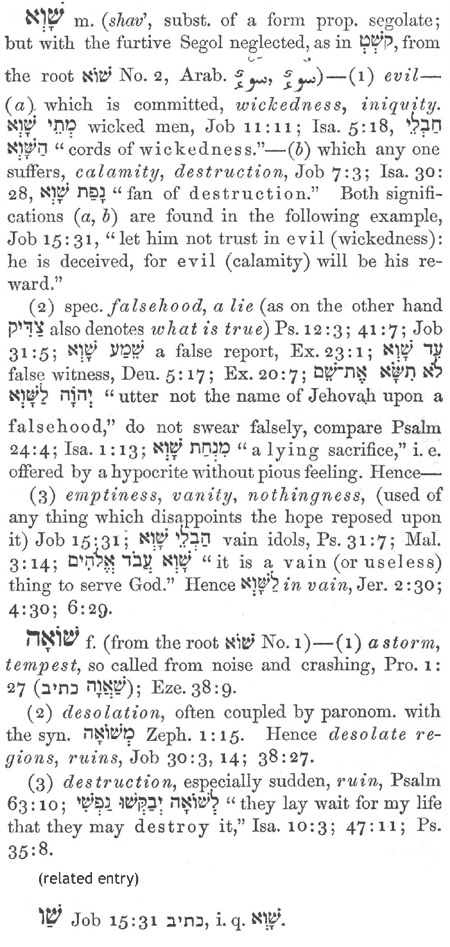
\includegraphics[width=10cm]{vain_hebrew}

H7723 corresponds to:\newline
'shav G459 a nomos\newline
shav G824 a topos\newline
shav G2756 kenos\newline
shav G3152 mataios\newline
shav G3153 mataiotes\newline
shav G3155 maten\newline
shav G3155 maten\newline
shav G5571 pseudes'\newline
\url{http://studybible.info/strongs/H7723}\newline


G5571 has G5574 as it's root. \newline
\url{https://www.blueletterbible.org/lang/lexicon/lexicon.cfm?Strongs=G5571&t=KJV}
\newline\newline
'3 But Peter said, “Ananias, why has Satan filled your heart to lie G5574 to the Holy Spirit and keep back part of the price of the land for yourself?'
(Acts 5)

This correspondence "vain" and "deceit" or "lies" can also be seen in the Septuagint other translations:

"You shall not circulate a false H7723 report. Do not put your hand with the wicked to be an unrighteous witness."\newline
(Exodus 23:1)

"You shall not welcome [2report 1a vain].G3152 You shall not assent together with the unjust to become [2witness 1an unjust]"\newline
(Exodus 23:1 Apostolic Bible Polyglot)\newline

G5574 is used for what happened in the case of Achane:\newline
'[3have sinned 1the 2people], and violated my covenant which I ordained with it. For even they took from the offering for consumption, and stealing they lie, G5574 and they cast [3for 1the 2items] themselves.'\newline
(Joshua 7:11 Apostolic Bible Polyglot)\newline

'Israel has sinned, and they have also transgressed My covenant which I commanded them. For they have even taken some of the accursed things, and have both stolen and deceived; H3584  and they have also put it among their own stuff.'\newline
(Joshua 7)\newline

\bibitem{holy spirit} 
"And take the helmet of salvation, and the sword of the Spirit, which is the word of God;" (Ephesians 6:17)

\bibitem{keep meaning} 
From the greek definition of G5442 we can see this means to guard 
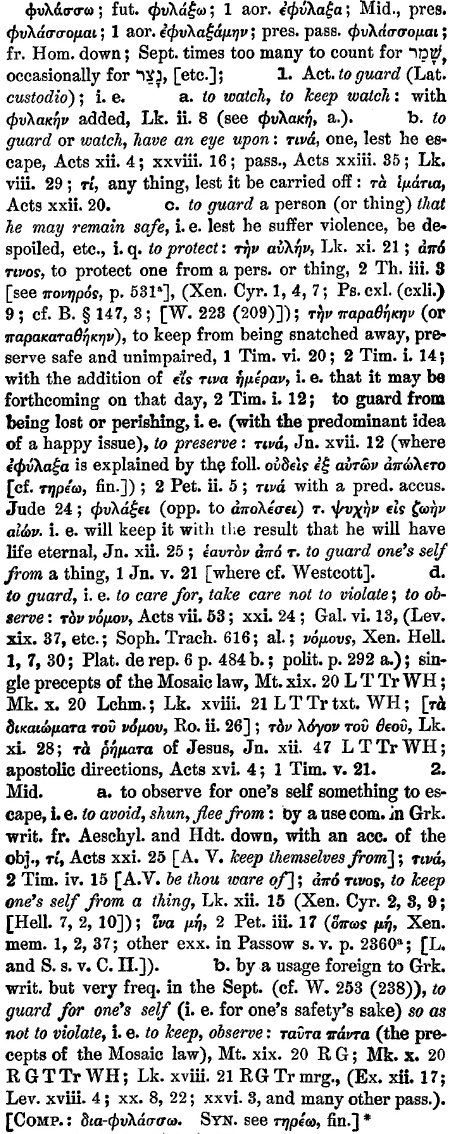
\includegraphics[width=8cm]{guard_greek}


 The Septuagint usage from this word in Luke 18:21 means to guard:
http://studybible.info/search-interlinear/strongs/g5442
Genesis 2:15
Genesis 3:24
Genesis 18:19
Genesis 26:5
Genesis 30:31
Genesis 31:24
Genesis 31:29
Genesis 41:35
Exodus 12:17
etc . . .

\bibitem{ruler} 
Ruler means ruler of a syngogue or a religious authority. Examples here in KJV:
 Luk 14:1
And it came to pass, as he went into the house of one of the chief G758 Pharisees to eat bread on the sabbath day, that they watched him.

 Luk 18:18
And a certain ruler G758 asked him, saying, Good Master, what shall I do to inherit eternal life?

 Luk 23:13
And Pilate, when he had called together the chief priests and the rulers G758 and the people,

 Luk 23:35
And the people stood beholding. And the rulers G758 also with them derided him, saying, He saved others; let him save himself, if he be Christ, the chosen of God.

 Luk 24:20
And how the chief priests and our rulers G758 delivered him to be condemned to death, and have crucified him.

 Jhn 3:1
There was a man of the Pharisees, named Nicodemus, a ruler G758 of the Jews:

 Jhn 7:26
But, lo, he speaketh boldly, and they say nothing unto him. Do the rulers G758 know indeed that this is the very Christ?

 Jhn 7:48
Have any of the rulers G758 or of the Pharisees believed on him?
\bibitem{possessions thayer's strong's} 
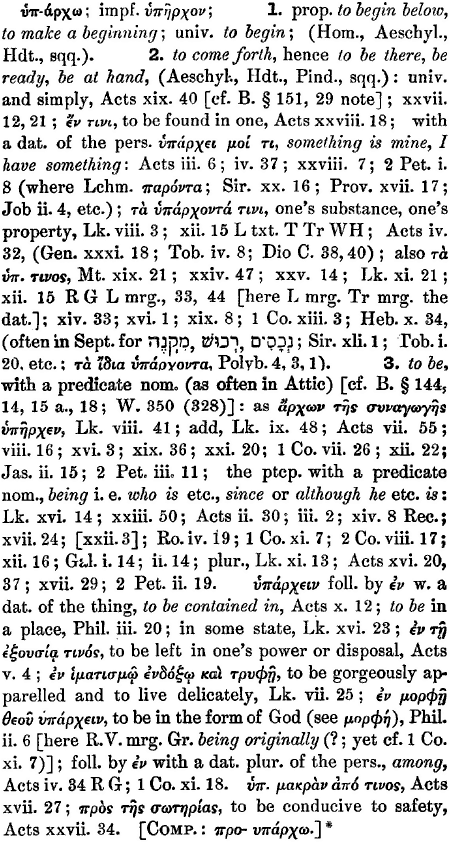
\includegraphics[width=10cm]{possessions}
Strong's:
ὑπάρχοντα
things extant or in hand, i.e. property 
\url{https://www.blueletterbible.org/lang/lexicon/lexicon.cfm?t=nasb&strongs=g5224}

\bibitem{G5224 apostolic bible polyglot} 
And according to the "Apostolic Bible Polyglot Greek-English Interline" G5224 can be translated as "existed"
2 Chronicles 26:10
. . . for [2cattle 1much] existed G5224 to him in Sephela . . .
\url{http://studybible.info/interlinear/2%20Chronicles%2026:10}

Lamentations 1:2
". . . and no one existed G5224 comforting her from all the ones loving her . . ."
\url{http://studybible.info/interlinear/Lamentations%201:2}


\bibitem{H4339}
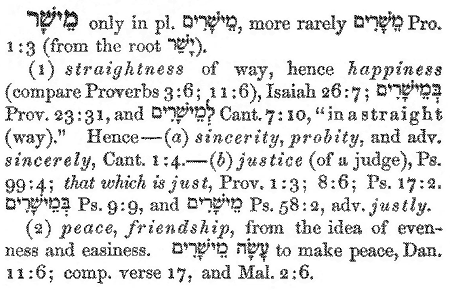
\includegraphics[width=10cm]{gesenius_h4339} 
 
 [מֵישָׁר]
 noun masculine evenness, uprightness, equity; — only plural: מֵשָׁרִים Proverbs 1:3; elsewhere מֵישָׁרִים Isaiah 26:7 17t.; —
1 evenness, level Isaiah 26:7, of path of righteous (in the future), figurative for free from difficulties; smoothness, of the flow of wine, ׳בְּמ Proverbs 23:31; ׳למ Song of Solomon 7:10.

2 in ethical sense, uprightness, equity, as taught in the school of wisdom Proverbs 8:6, "" צֶדֶק Proverbs 1:3; Proverbs 2:9; of government ׳(ב)מ Psalm 9:9; Psalm 58:2; Psalm 75:3; Psalm 96:10; Psalm 99:4; of speech Isaiah 33:15; Proverbs 23:16; of Yahweh's promises Isaiah 45:19; ׳רצה מ 1 Chronicles 29:17 have pleasure in equity; ׳עשׂה מ Daniel 11:6 make an equitable arrangement.

3 adverb rightly, with חזה Psalm 17:2; אהב Song of Solomon 1:4.

Brown-Driver-Briggs Hebrew and English Lexicon, Unabridged, Electronic Database.
Copyright © 2002, 2003, 2006 by Biblesoft, Inc. 
All rights reserved. Used by permission. BibleSoft.com
usage (KJV)

1Ch 29:17
I know also, my God, that thou triest the heart, and hast pleasure in uprightness. As for me, in the uprightness H4339 of mine heart I have willingly offered all these things: and now have I seen with joy thy people, which are present here, to offer willingly unto thee.

Psa 9:8
And he shall judge the world in righteousness, he shall minister judgment to the people in uprightness. H4339

Psa 17:2
Let my sentence come forth from thy presence; let thine eyes behold the things that are equal. H4339

Psa 58:1
[[To the chief Musician, Altaschith, Michtam of David.]] Do ye indeed speak righteousness, O congregation? do ye judge uprightly, H4339 O ye sons of men?

Psa 75:2
When I shall receive the congregation I will judge uprightly. H4339

Psa 96:10
Say among the heathen that the LORD reigneth: the world also shall be established that it shall not be moved: he shall judge the people righteously. H4339

Psa 98:9
Before the LORD; for he cometh to judge the earth: with righteousness shall he judge the world, and the people with equity. H4339

Psa 99:4
The king's strength also loveth judgment; thou dost establish equity, H4339 thou executest judgment and righteousness in Jacob.

Pro 1:3
To receive the instruction of wisdom, justice, and judgment, and equity; H4339

Pro 2:9
Then shalt thou understand righteousness, and judgment, and equity; H4339 yea, every good path.

Pro 8:6
Hear; for I will speak of excellent things; and the opening of my lips shall be right things. H4339

Pro 23:16
Yea, my reins shall rejoice, when thy lips speak right things. H4339

Pro 23:31
Look not thou upon the wine when it is red, when it giveth his colour in the cup, when it moveth itself aright. H4339

Sng 1:4
Draw me, we will run after thee: the king hath brought me into his chambers: we will be glad and rejoice in thee, we will remember thy love more than wine: the upright H4339 love thee.

Sng 7:9
And the roof of thy mouth like the best wine for my beloved, that goeth down sweetly, H4339 causing the lips of those that are asleep to speak.

Isa 26:7
The way of the just is uprightness: H4339 thou, most upright, dost weigh the path of the just.

Isa 33:15
He that walketh righteously, and speaketh uprightly; H4339 he that despiseth the gain of oppressions, that shaketh his hands from holding of bribes, that stoppeth his ears from hearing of blood, and shutteth his eyes from seeing evil;

Isa 45:19
I have not spoken in secret, in a dark place of the earth: I said not unto the seed of Jacob, Seek ye me in vain: I the LORD speak righteousness, I declare things that are right. H4339

Dan 11:6
And in the end of years they shall join themselves together; for the king's daughter of the south shall come to the king of the north to make an agreement: H4339 but she shall not retain the power of the arm; neither shall he stand, nor his arm: but she shall be given up, and they that brought her, and he that begat her, and he that strengthened her in these times.


\bibitem{the poor}
http://biblehub.com/commentaries/ellicott/galatians/2.htm
Ellicott's Commentary for English Readers
Galatians 2:10
Only they would that we should remember the poor; the same which I also was forward to do.
(10) The poor—i.e., at Jerusalem and in Judaea. St. Paul had already been the means of bringing contributions from the wealthier churches of Antioch to Jerusalem (Acts 11:29-30). This seems to have been gracefully received, not only as an act of charity, but as a recognition of the claims of the mother Church. The Apostles expressed a hope that the same good feeling might continue, to which St. Paul willingly assented. That he did not forget his promise appears from Acts 24:17; Romans 15:26-27; 1Corinthians 16:3; 2Corinthians 8:1-2; 2Corinthians 9:1 et sea. (See Notes on Romans 15:25-27.)


\bibitem{common faith}
It uses the same word for "common" property to talk about the "common" faith. It is used both as "common" in terms of shared and "common" in terms of unholy, just as the things that Achan had were both types of devoted. The new testament usage follows:

\begin{greek}
Mark 7:2 Adj-DFP
GRK: αὐτοῦ ὅτι κοιναῖς χερσίν τοῦτ'
NAS: their bread with impure hands,
KJV: bread with defiled, that is to say,
INT: of him that with defiled hands that

Mark 7:5 Adj-DFP
GRK: πρεσβυτέρων ἀλλὰ κοιναῖς χερσὶν ἐσθίουσιν
NAS: their bread with impure hands?
INT: elders but with unwashed hands eat

Acts 2:44 Adj-ANP
GRK: εἶχον ἅπαντα κοινά 
NAS: and had all things in common;
KJV: had all things common;
INT: having all things in common

Acts 4:32 Adj-NNP
GRK: αὐτοῖς ἅπαντα κοινά 
NAS: but all things were common property to them.
KJV: had all things common.
INT: to them all things common

Acts 10:14 Adj-ANS
GRK: ἔφαγον πᾶν κοινὸν καὶ ἀκάθαρτον
NAS: eaten anything unholy and unclean.
KJV: any thing that is common or
INT: did I eat anything common or unclean

Acts 10:28 Adj-AMS
GRK: ἔδειξεν μηδένα κοινὸν ἢ ἀκάθαρτον
NAS: any man unholy or unclean.
KJV: any man common or unclean.
INT: showed not common or unclean

Acts 11:8 Adj-ANS
GRK: κύριε ὅτι κοινὸν ἢ ἀκάθαρτον
NAS: Lord, for nothing unholy or unclean
KJV: for nothing common or unclean
INT: Lord for common or unclean

Romans 14:14 Adj-NNS
GRK: ὅτι οὐδὲν κοινὸν δι' ἑαυτοῦ
NAS: that nothing is unclean in itself;
KJV: [there is] nothing unclean of
INT: that nothing [is] unclean of itself

Romans 14:14 Adj-ANS
GRK: λογιζομένῳ τι κοινὸν εἶναι ἐκείνῳ
NAS: anything to be unclean, to him it is unclean.
KJV: to be unclean, to him
INT: reckons anything unclean to be to that one

Romans 14:14 Adj-NNS
GRK: εἶναι ἐκείνῳ κοινόν 
NAS: to be unclean, to him it is unclean.
KJV: unclean, to him [it is] unclean.
INT: to be to that one unclean [it is]

Titus 1:4 Adj-AFS
GRK: τέκνῳ κατὰ κοινὴν πίστιν χάρις
NAS: my TRUE child in a common faith: Grace
KJV: son after the common faith: Grace,
INT: child according to [our] common faith Grace

Hebrews 10:29 Adj-ANS
GRK: τῆς διαθήκης κοινὸν ἡγησάμενος ἐν
NAS: and has regarded as unclean the blood
KJV: he was sanctified, an unholy thing, and
INT: of the covenant common having esteemed in

Jude 1:3 Adj-GFS
GRK: περὶ τῆς κοινῆς ἡμῶν σωτηρίας
NAS: you about our common salvation,
KJV: of the common salvation,
INT: concerning the common of us salvation

Revelation 21:27 Adj-NNS
GRK: αὐτὴν πᾶν κοινὸν καὶ ὁ
NAS: and nothing unclean, and no
INT: it anything defiling and those
\end{greek}
\url{http://biblehub.com/greek/strongs_2839.htm}

There is not any significant difference in the Old Testament usage:
\url{http://studybible.info/search-interlinear/strongs/G2839}


\bibitem{koinos}
One example of it's usage is in Greek literature is:
"common things, the things of friends"
\begin{greek}
“κοινὰ τὰ τῶν φίλων” E.Or.735 (troch.), Pl.Phdr.279c, Men.9, etc.

And anouther would be "jointly"

B. Adv. κοινῶς in common, jointly, E.Ion1462; “τὰ κοινὰ κ. δεῖ φέρειν συμπτώματα” Men.817: Comp., ἐν Κρήτῃ -οτέρως [ἔχει τὰ τῶν συσσιτίων] Arist.Pol.1272a16.

for full usage see:
\url{http://www.perseus.tufts.edu/hopper/text?doc=Perseus:text:1999.04.0057:entry=koino/s}
\end{greek}

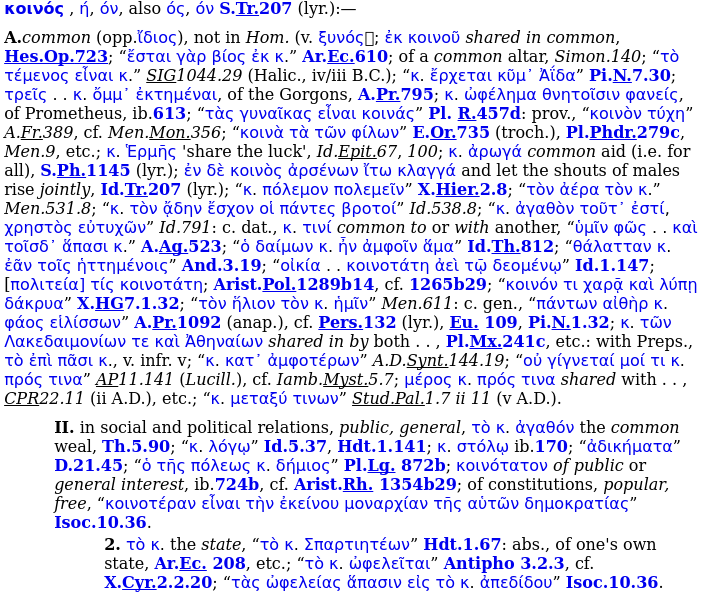
\includegraphics[width=12cm]{koinos1}
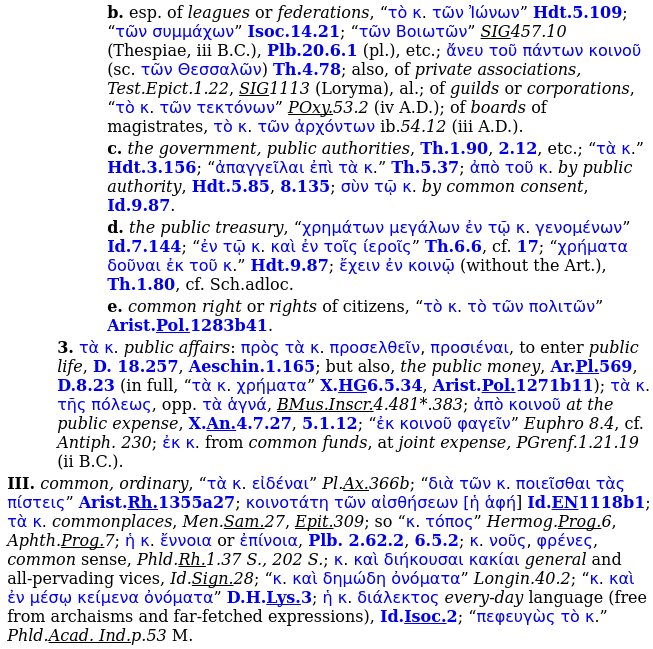
\includegraphics[width=12cm]{koinos2}
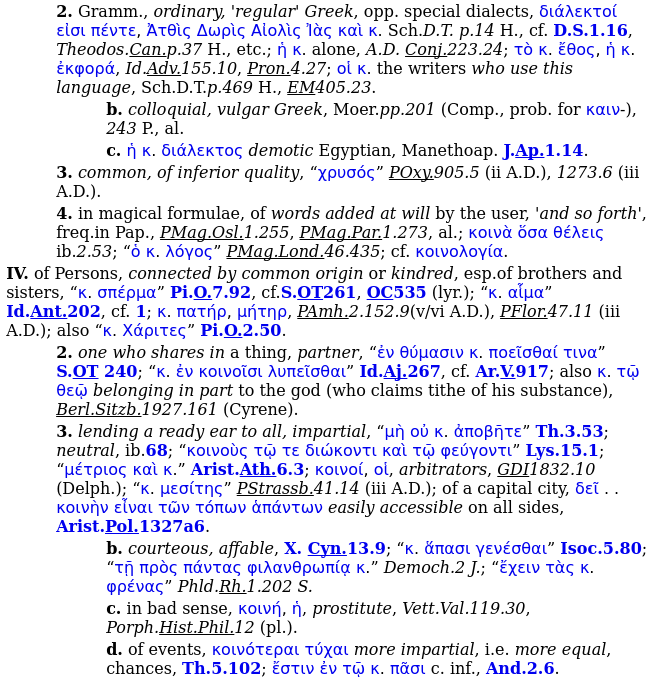
\includegraphics[width=12cm]{koinos3}
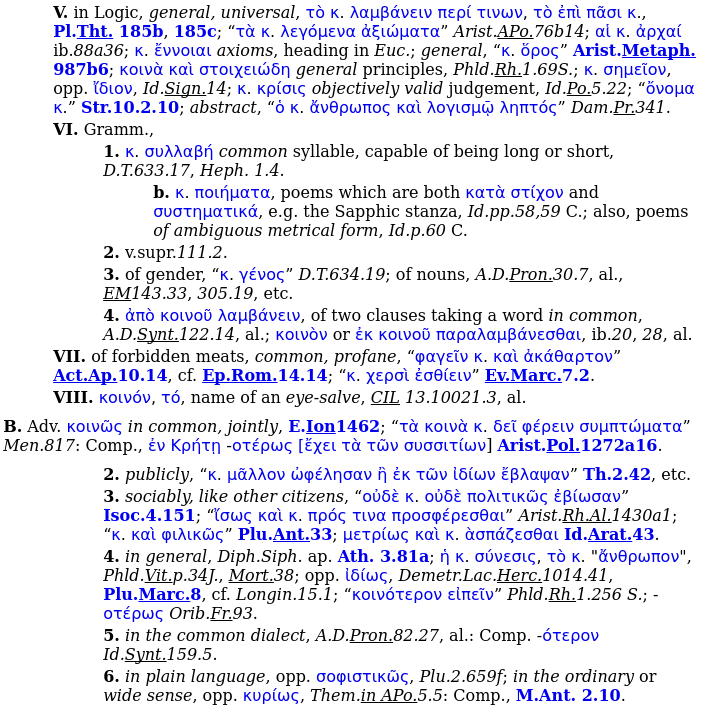
\includegraphics[width=12cm]{koinos4}
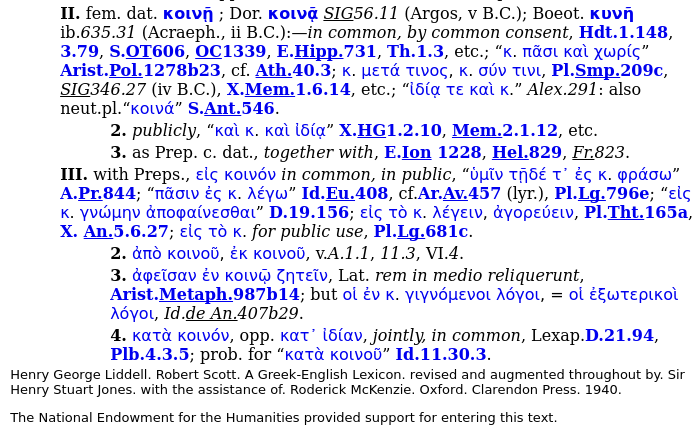
\includegraphics[width=12cm]{koinos5}

\bibitem{H2764 H2763}
Outline of Biblical Usage\newline
a thing devoted, thing dedicated, ban, devotion
a net, thing perforated
have been utterly destroyed, (appointed to) utter destruction\newline
\url{https://www.blueletterbible.org/lang/lexicon/lexicon.cfm?Strongs=H2764&t=KJV}
\newline
H2764\begin{hebrew}(חֵרֶם)\end{hebrew} has as it's root: H2763\begin{hebrew}(חָרַם)\end{hebrew} \newline
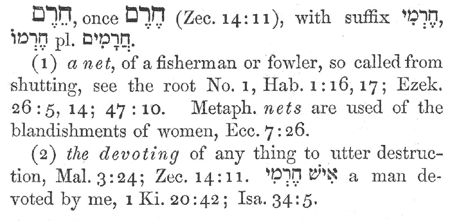
\includegraphics[width=12cm]{H2764}
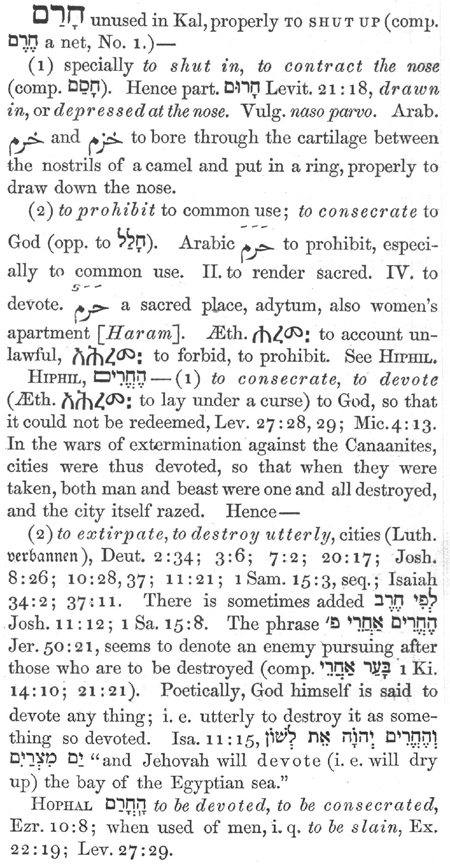
\includegraphics[width=12cm]{H2763}

\bibitem{hate means love less}
Robinson, Rich. “Did Jesus Teach His Disciples to Hate Their Parents?” Jews for Jesus, Jews For Jesus, 1 Jan. 2000, Accessed 12 Aug. 2017 jewsforjesus.org/answers/did-jesus-teach-his-disciples-to-hate-their-parents/.

\bibitem{gospel coalition}
'Acts 2-5 portrays a spirit of communal sharing rather than an actual commune. The people did not sell everything they owned to legal title, as those typically do in a commune. This is evidenced by the imperfect verbs used throughout the passages. Craig Blomberg says in his study Neither Poverty nor Riches, “[Chapter 2] verses 43-47 are dominated by highly marked imperfect tense verbs, whereas one normally expects aorists [once-for-all actions] in historical narrative. There is no once-for-all divestiture of property in view here, but periodic acts of charity as needs arose.”

This point is even clearer in Acts 4-5. The NIV translation of Acts 4:34b-35 says, “From time to time, those who owned land or houses sold them, brought the money from the sales and put it at the apostles’ feet.” Blomberg comments:

Again we have a rash of imperfect verbs here, this time explicitly reflected in the NIV’s “from time to time.” The periodic selling of property confirms our interpretation of Acts 2:44 above. This was not a one-time divesture of all one’s possessions. The theme “according to need,” reappears, too. Interestingly, what does not appear in this paragraph is any statement of complete equality among believers.'

Lindsley, Art. “Does the Book of Acts Command Socialism?” The Gospel Coalition, The Gospel Coalition, 28 May 2013, \url{https://www.thegospelcoalition.org/article/does-the-book-of-acts-command-socialism} . 

\bibitem{habit selling possessions}
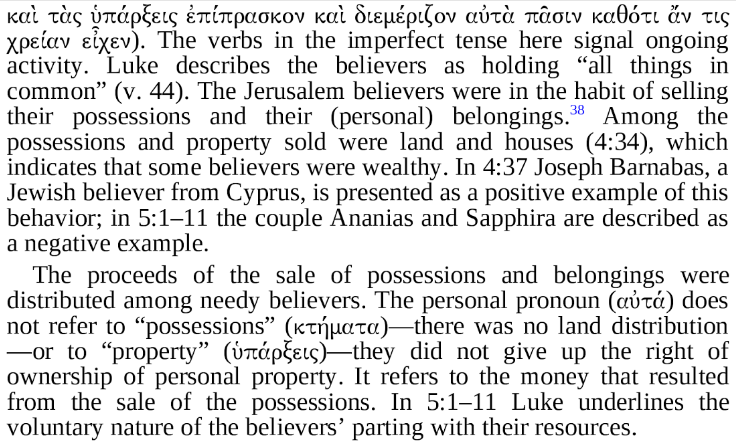
\includegraphics[width=12cm]{eckhard_habit_selling_possessions}
Schnabel, Eckhard J. Acts. Zondervan, 2012, \url{books.google.com/books?id=fjD9CwAAQBAJ&pg=PT250}.

\bibitem{slaughter and sacrifice}
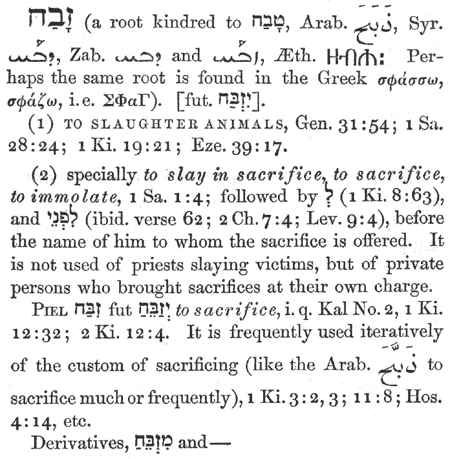
\includegraphics[width=12cm]{slaughter_sacrifice_2076}
\url{https://www.blueletterbible.org/lang/lexicon/lexicon.cfm?Strongs=H2076&t=KJV}
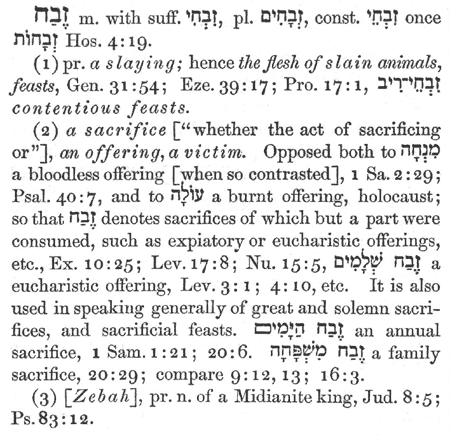
\includegraphics[width=12cm]{slaughter_sacrifice_2077}
\url{https://www.blueletterbible.org/lang/lexicon/lexicon.cfm?Strongs=H2077&t=KJV}

\bibitem{jussive mood kd}
Keil and Delitzsch OT Commentary
Deuteronomy 15:4
Save when there shall be no poor among you; for the LORD shall greatly bless thee in the land which the LORD thy God giveth thee for an inheritance to possess it:
"Only that there shall be no poor with thee." יהיה is jussive, like the foregoing imperfects. The meaning in this connection is, "Thou needest not to remit a debt to foreigners in the seventh year; thou hast only to take care that there is no poor man with or among thee, that thou dost not cause or increase their poverty, by oppressing the brethren who have borrowed of thee." Understood in this way, the sentence is not at all at variance with Deuteronomy 15:11, where it is stated that the poor would never cease out of the land. The following clause, "for Jehovah will bless thee," etc., gives a reason for the main thought, that they were not to press the Israelitish debtor. The creditor, therefore, had no need to fear that he would suffer want, if he refrained from exacting his debt from his brother in the seventh year. 
\url{http://biblehub.com/commentaries/kad/deuteronomy/15.htm}

\bibitem{niehaus}
'But the language
of Deuteronomy 12:5 need not be pressed so far. The command says
that they must bring ‘your burnt offerings and sacrifices, your tithes
and special gifts, what you have vowed to give and your freewill
offerings, and the firstborn of your herds and flocks’. The list may
sound exhaustive, but it is not. As Mayes notes, ‘the list of offerings
and sacrifices, apparently intended to be comprehensive, makes no
reference to the sin and guilt offerings (Lv. 4:1ff)’.22 The list is a general one, and given for emphasis, not for exclusivity. The
statement may be taken as an example of Ancient Near Eastern
hyperbole—never meant to be taken quite literally, always meant to
emphasize a point.' from page 8-9 of: \newline
Niehaus, Jeffrey. “THE CENTRAL SANCTUARY: WHERE AND WHEN?” Tyndale Bulletin, vol. 43, no. 1, May 1992, pp. 3–30.
\url{http://www.tyndalehouse.com/tynbul/library/TynBull_1992_43_1_01_Niehaus_CentralSanctuary.pdf}

\bibitem{ellen white}
"Therefore, one must determine why the bamot are so problematic. The most convincing theory is that after the Temple was built in Jerusalem, it was no longer appropriate to worship elsewhere (1 Kings 3:2), especially in light of Deuteronomy 12.23 However, when exactly this was understood by historical Israel is harder to determine. Richard D. Nelson of the Perkins School of Theology claims that this is to set the worship of Yahweh apart from the worship of Baal: “The plurality of shrines inevitably reflected the local multiplicity of Canaanite Baal worship, implying a Yahweh of Dan and another Yahweh at Bethel.”24 Theological heavyweight Walter Brueggeman concurs with this analysis and says that these shrines compromised Yahweh’s jealous claim to Israel.25 This does not mean that those who were living in Israel during the monarchal period would have recognized this shift, but that the condemnation is a reflection of the author/redactor’s theology.26"
. . . 
"Jeffery J. Niehaus of Gordon-Conwell Theological Seminary says, “The Carmel event clearly shows that Yahweh can approve a sacrifice not offered at the ‘chosen place,’ and in a most dramatic way, when it is offered in a special context and for a special purpose.” Yet, the bamot are not “special” as in unique or uncommon; they are a place of ongoing regular worship. Therefore, the example of Carmel only heightens the contrast between a special theophanic event and an ongoing part of the cult, which demonstrates a stage in the development of centralization."
White, Ellen. “High Places, Altars and the Bamah.” Biblical Archaeology Society, Biblical Archaeology Society, 26 May 2017, www.biblicalarchaeology.org/daily/ancient-cultures/ancient-israel/high-places-altars-and-the-bamah/.

\bibitem{shatnez}
"Josephus describes the belt as being hollow like the skin shed by a snake (Antiquities 3:7:2). It was a work of "embroidery;" when used in this context of Temple furnishings, the Bible uses this term to indicate that the same design was featured on both sides of the material. Although the belt itself was made of linen, the embroidery-a floral design-was done of colored wool threads (the three colors which we have mentioned), and attached to the white linen background. This combination of wool and linen together in garments is normally forbidden (see Lev. 19:19), but it was permitted for the priestly garments."
“Preistly Garments.” The Temple Institute: The Priestly Garments: The Belt, Temple Institute, \url{www.templeinstitute.org/beged/priestly_garments-11.htm}.


\bibitem{renounce}
“Renounce.” Merriam-Webster, Merriam-Webster, \url{www.merriam-webster.com/dictionary/renounce}. Last accessed 08/28/2017.

\bibitem{seeskin}
Seeskin, Kenneth. Thinking about the Torah: a Philosopher Reads the Bible. The Jewish Publication Society, 2016.
\end{thebibliography}

\section{GNU Free Documentation License}

                GNU Free Documentation License
                 Version 1.3, 3 November 2008


 Copyright (C) 2000, 2001, 2002, 2007, 2008 Free Software Foundation, Inc.
     <https://fsf.org/>
 Everyone is permitted to copy and distribute verbatim copies
 of this license document, but changing it is not allowed.

0. PREAMBLE

The purpose of this License is to make a manual, textbook, or other
functional and useful document "free" in the sense of freedom: to
assure everyone the effective freedom to copy and redistribute it,
with or without modifying it, either commercially or noncommercially.
Secondarily, this License preserves for the author and publisher a way
to get credit for their work, while not being considered responsible
for modifications made by others.

This License is a kind of "copyleft", which means that derivative
works of the document must themselves be free in the same sense.  It
complements the GNU General Public License, which is a copyleft
license designed for free software.

We have designed this License in order to use it for manuals for free
software, because free software needs free documentation: a free
program should come with manuals providing the same freedoms that the
software does.  But this License is not limited to software manuals;
it can be used for any textual work, regardless of subject matter or
whether it is published as a printed book.  We recommend this License
principally for works whose purpose is instruction or reference.


1. APPLICABILITY AND DEFINITIONS

This License applies to any manual or other work, in any medium, that
contains a notice placed by the copyright holder saying it can be
distributed under the terms of this License.  Such a notice grants a
world-wide, royalty-free license, unlimited in duration, to use that
work under the conditions stated herein.  The "Document", below,
refers to any such manual or work.  Any member of the public is a
licensee, and is addressed as "you".  You accept the license if you
copy, modify or distribute the work in a way requiring permission
under copyright law.

A "Modified Version" of the Document means any work containing the
Document or a portion of it, either copied verbatim, or with
modifications and/or translated into another language.

A "Secondary Section" is a named appendix or a front-matter section of
the Document that deals exclusively with the relationship of the
publishers or authors of the Document to the Document's overall
subject (or to related matters) and contains nothing that could fall
directly within that overall subject.  (Thus, if the Document is in
part a textbook of mathematics, a Secondary Section may not explain
any mathematics.)  The relationship could be a matter of historical
connection with the subject or with related matters, or of legal,
commercial, philosophical, ethical or political position regarding
them.

The "Invariant Sections" are certain Secondary Sections whose titles
are designated, as being those of Invariant Sections, in the notice
that says that the Document is released under this License.  If a
section does not fit the above definition of Secondary then it is not
allowed to be designated as Invariant.  The Document may contain zero
Invariant Sections.  If the Document does not identify any Invariant
Sections then there are none.

The "Cover Texts" are certain short passages of text that are listed,
as Front-Cover Texts or Back-Cover Texts, in the notice that says that
the Document is released under this License.  A Front-Cover Text may
be at most 5 words, and a Back-Cover Text may be at most 25 words.

A "Transparent" copy of the Document means a machine-readable copy,
represented in a format whose specification is available to the
general public, that is suitable for revising the document
straightforwardly with generic text editors or (for images composed of
pixels) generic paint programs or (for drawings) some widely available
drawing editor, and that is suitable for input to text formatters or
for automatic translation to a variety of formats suitable for input
to text formatters.  A copy made in an otherwise Transparent file
format whose markup, or absence of markup, has been arranged to thwart
or discourage subsequent modification by readers is not Transparent.
An image format is not Transparent if used for any substantial amount
of text.  A copy that is not "Transparent" is called "Opaque".

Examples of suitable formats for Transparent copies include plain
ASCII without markup, Texinfo input format, LaTeX input format, SGML
or XML using a publicly available DTD, and standard-conforming simple
HTML, PostScript or PDF designed for human modification.  Examples of
transparent image formats include PNG, XCF and JPG.  Opaque formats
include proprietary formats that can be read and edited only by
proprietary word processors, SGML or XML for which the DTD and/or
processing tools are not generally available, and the
machine-generated HTML, PostScript or PDF produced by some word
processors for output purposes only.

The "Title Page" means, for a printed book, the title page itself,
plus such following pages as are needed to hold, legibly, the material
this License requires to appear in the title page.  For works in
formats which do not have any title page as such, "Title Page" means
the text near the most prominent appearance of the work's title,
preceding the beginning of the body of the text.

The "publisher" means any person or entity that distributes copies of
the Document to the public.

A section "Entitled XYZ" means a named subunit of the Document whose
title either is precisely XYZ or contains XYZ in parentheses following
text that translates XYZ in another language.  (Here XYZ stands for a
specific section name mentioned below, such as "Acknowledgements",
"Dedications", "Endorsements", or "History".)  To "Preserve the Title"
of such a section when you modify the Document means that it remains a
section "Entitled XYZ" according to this definition.

The Document may include Warranty Disclaimers next to the notice which
states that this License applies to the Document.  These Warranty
Disclaimers are considered to be included by reference in this
License, but only as regards disclaiming warranties: any other
implication that these Warranty Disclaimers may have is void and has
no effect on the meaning of this License.

2. VERBATIM COPYING

You may copy and distribute the Document in any medium, either
commercially or noncommercially, provided that this License, the
copyright notices, and the license notice saying this License applies
to the Document are reproduced in all copies, and that you add no
other conditions whatsoever to those of this License.  You may not use
technical measures to obstruct or control the reading or further
copying of the copies you make or distribute.  However, you may accept
compensation in exchange for copies.  If you distribute a large enough
number of copies you must also follow the conditions in section 3.

You may also lend copies, under the same conditions stated above, and
you may publicly display copies.


3. COPYING IN QUANTITY

If you publish printed copies (or copies in media that commonly have
printed covers) of the Document, numbering more than 100, and the
Document's license notice requires Cover Texts, you must enclose the
copies in covers that carry, clearly and legibly, all these Cover
Texts: Front-Cover Texts on the front cover, and Back-Cover Texts on
the back cover.  Both covers must also clearly and legibly identify
you as the publisher of these copies.  The front cover must present
the full title with all words of the title equally prominent and
visible.  You may add other material on the covers in addition.
Copying with changes limited to the covers, as long as they preserve
the title of the Document and satisfy these conditions, can be treated
as verbatim copying in other respects.

If the required texts for either cover are too voluminous to fit
legibly, you should put the first ones listed (as many as fit
reasonably) on the actual cover, and continue the rest onto adjacent
pages.

If you publish or distribute Opaque copies of the Document numbering
more than 100, you must either include a machine-readable Transparent
copy along with each Opaque copy, or state in or with each Opaque copy
a computer-network location from which the general network-using
public has access to download using public-standard network protocols
a complete Transparent copy of the Document, free of added material.
If you use the latter option, you must take reasonably prudent steps,
when you begin distribution of Opaque copies in quantity, to ensure
that this Transparent copy will remain thus accessible at the stated
location until at least one year after the last time you distribute an
Opaque copy (directly or through your agents or retailers) of that
edition to the public.

It is requested, but not required, that you contact the authors of the
Document well before redistributing any large number of copies, to
give them a chance to provide you with an updated version of the
Document.


4. MODIFICATIONS

You may copy and distribute a Modified Version of the Document under
the conditions of sections 2 and 3 above, provided that you release
the Modified Version under precisely this License, with the Modified
Version filling the role of the Document, thus licensing distribution
and modification of the Modified Version to whoever possesses a copy
of it.  In addition, you must do these things in the Modified Version:

A. Use in the Title Page (and on the covers, if any) a title distinct
   from that of the Document, and from those of previous versions
   (which should, if there were any, be listed in the History section
   of the Document).  You may use the same title as a previous version
   if the original publisher of that version gives permission.
B. List on the Title Page, as authors, one or more persons or entities
   responsible for authorship of the modifications in the Modified
   Version, together with at least five of the principal authors of the
   Document (all of its principal authors, if it has fewer than five),
   unless they release you from this requirement.
C. State on the Title page the name of the publisher of the
   Modified Version, as the publisher.
D. Preserve all the copyright notices of the Document.
E. Add an appropriate copyright notice for your modifications
   adjacent to the other copyright notices.
F. Include, immediately after the copyright notices, a license notice
   giving the public permission to use the Modified Version under the
   terms of this License, in the form shown in the Addendum below.
G. Preserve in that license notice the full lists of Invariant Sections
   and required Cover Texts given in the Document's license notice.
H. Include an unaltered copy of this License.
I. Preserve the section Entitled "History", Preserve its Title, and add
   to it an item stating at least the title, year, new authors, and
   publisher of the Modified Version as given on the Title Page.  If
   there is no section Entitled "History" in the Document, create one
   stating the title, year, authors, and publisher of the Document as
   given on its Title Page, then add an item describing the Modified
   Version as stated in the previous sentence.
J. Preserve the network location, if any, given in the Document for
   public access to a Transparent copy of the Document, and likewise
   the network locations given in the Document for previous versions
   it was based on.  These may be placed in the "History" section.
   You may omit a network location for a work that was published at
   least four years before the Document itself, or if the original
   publisher of the version it refers to gives permission.
K. For any section Entitled "Acknowledgements" or "Dedications",
   Preserve the Title of the section, and preserve in the section all
   the substance and tone of each of the contributor acknowledgements
   and/or dedications given therein.
L. Preserve all the Invariant Sections of the Document,
   unaltered in their text and in their titles.  Section numbers
   or the equivalent are not considered part of the section titles.
M. Delete any section Entitled "Endorsements".  Such a section
   may not be included in the Modified Version.
N. Do not retitle any existing section to be Entitled "Endorsements"
   or to conflict in title with any Invariant Section.
O. Preserve any Warranty Disclaimers.

If the Modified Version includes new front-matter sections or
appendices that qualify as Secondary Sections and contain no material
copied from the Document, you may at your option designate some or all
of these sections as invariant.  To do this, add their titles to the
list of Invariant Sections in the Modified Version's license notice.
These titles must be distinct from any other section titles.

You may add a section Entitled "Endorsements", provided it contains
nothing but endorsements of your Modified Version by various
parties--for example, statements of peer review or that the text has
been approved by an organization as the authoritative definition of a
standard.

You may add a passage of up to five words as a Front-Cover Text, and a
passage of up to 25 words as a Back-Cover Text, to the end of the list
of Cover Texts in the Modified Version.  Only one passage of
Front-Cover Text and one of Back-Cover Text may be added by (or
through arrangements made by) any one entity.  If the Document already
includes a cover text for the same cover, previously added by you or
by arrangement made by the same entity you are acting on behalf of,
you may not add another; but you may replace the old one, on explicit
permission from the previous publisher that added the old one.

The author(s) and publisher(s) of the Document do not by this License
give permission to use their names for publicity for or to assert or
imply endorsement of any Modified Version.


5. COMBINING DOCUMENTS

You may combine the Document with other documents released under this
License, under the terms defined in section 4 above for modified
versions, provided that you include in the combination all of the
Invariant Sections of all of the original documents, unmodified, and
list them all as Invariant Sections of your combined work in its
license notice, and that you preserve all their Warranty Disclaimers.

The combined work need only contain one copy of this License, and
multiple identical Invariant Sections may be replaced with a single
copy.  If there are multiple Invariant Sections with the same name but
different contents, make the title of each such section unique by
adding at the end of it, in parentheses, the name of the original
author or publisher of that section if known, or else a unique number.
Make the same adjustment to the section titles in the list of
Invariant Sections in the license notice of the combined work.

In the combination, you must combine any sections Entitled "History"
in the various original documents, forming one section Entitled
"History"; likewise combine any sections Entitled "Acknowledgements",
and any sections Entitled "Dedications".  You must delete all sections
Entitled "Endorsements".


6. COLLECTIONS OF DOCUMENTS

You may make a collection consisting of the Document and other
documents released under this License, and replace the individual
copies of this License in the various documents with a single copy
that is included in the collection, provided that you follow the rules
of this License for verbatim copying of each of the documents in all
other respects.

You may extract a single document from such a collection, and
distribute it individually under this License, provided you insert a
copy of this License into the extracted document, and follow this
License in all other respects regarding verbatim copying of that
document.


7. AGGREGATION WITH INDEPENDENT WORKS

A compilation of the Document or its derivatives with other separate
and independent documents or works, in or on a volume of a storage or
distribution medium, is called an "aggregate" if the copyright
resulting from the compilation is not used to limit the legal rights
of the compilation's users beyond what the individual works permit.
When the Document is included in an aggregate, this License does not
apply to the other works in the aggregate which are not themselves
derivative works of the Document.

If the Cover Text requirement of section 3 is applicable to these
copies of the Document, then if the Document is less than one half of
the entire aggregate, the Document's Cover Texts may be placed on
covers that bracket the Document within the aggregate, or the
electronic equivalent of covers if the Document is in electronic form.
Otherwise they must appear on printed covers that bracket the whole
aggregate.


8. TRANSLATION

Translation is considered a kind of modification, so you may
distribute translations of the Document under the terms of section 4.
Replacing Invariant Sections with translations requires special
permission from their copyright holders, but you may include
translations of some or all Invariant Sections in addition to the
original versions of these Invariant Sections.  You may include a
translation of this License, and all the license notices in the
Document, and any Warranty Disclaimers, provided that you also include
the original English version of this License and the original versions
of those notices and disclaimers.  In case of a disagreement between
the translation and the original version of this License or a notice
or disclaimer, the original version will prevail.

If a section in the Document is Entitled "Acknowledgements",
"Dedications", or "History", the requirement (section 4) to Preserve
its Title (section 1) will typically require changing the actual
title.


9. TERMINATION

You may not copy, modify, sublicense, or distribute the Document
except as expressly provided under this License.  Any attempt
otherwise to copy, modify, sublicense, or distribute it is void, and
will automatically terminate your rights under this License.

However, if you cease all violation of this License, then your license
from a particular copyright holder is reinstated (a) provisionally,
unless and until the copyright holder explicitly and finally
terminates your license, and (b) permanently, if the copyright holder
fails to notify you of the violation by some reasonable means prior to
60 days after the cessation.

Moreover, your license from a particular copyright holder is
reinstated permanently if the copyright holder notifies you of the
violation by some reasonable means, this is the first time you have
received notice of violation of this License (for any work) from that
copyright holder, and you cure the violation prior to 30 days after
your receipt of the notice.

Termination of your rights under this section does not terminate the
licenses of parties who have received copies or rights from you under
this License.  If your rights have been terminated and not permanently
reinstated, receipt of a copy of some or all of the same material does
not give you any rights to use it.


10. FUTURE REVISIONS OF THIS LICENSE

The Free Software Foundation may publish new, revised versions of the
GNU Free Documentation License from time to time.  Such new versions
will be similar in spirit to the present version, but may differ in
detail to address new problems or concerns.  See
https://www.gnu.org/licenses/.

Each version of the License is given a distinguishing version number.
If the Document specifies that a particular numbered version of this
License "or any later version" applies to it, you have the option of
following the terms and conditions either of that specified version or
of any later version that has been published (not as a draft) by the
Free Software Foundation.  If the Document does not specify a version
number of this License, you may choose any version ever published (not
as a draft) by the Free Software Foundation.  If the Document
specifies that a proxy can decide which future versions of this
License can be used, that proxy's public statement of acceptance of a
version permanently authorizes you to choose that version for the
Document.

11. RELICENSING

"Massive Multiauthor Collaboration Site" (or "MMC Site") means any
World Wide Web server that publishes copyrightable works and also
provides prominent facilities for anybody to edit those works.  A
public wiki that anybody can edit is an example of such a server.  A
"Massive Multiauthor Collaboration" (or "MMC") contained in the site
means any set of copyrightable works thus published on the MMC site.

"CC-BY-SA" means the Creative Commons Attribution-Share Alike 3.0 
license published by Creative Commons Corporation, a not-for-profit 
corporation with a principal place of business in San Francisco, 
California, as well as future copyleft versions of that license 
published by that same organization.

"Incorporate" means to publish or republish a Document, in whole or in 
part, as part of another Document.

An MMC is "eligible for relicensing" if it is licensed under this 
License, and if all works that were first published under this License 
somewhere other than this MMC, and subsequently incorporated in whole or 
in part into the MMC, (1) had no cover texts or invariant sections, and 
(2) were thus incorporated prior to November 1, 2008.

The operator of an MMC Site may republish an MMC contained in the site
under CC-BY-SA on the same site at any time before August 1, 2009,
provided the MMC is eligible for relicensing.


ADDENDUM: How to use this License for your documents

To use this License in a document you have written, include a copy of
the License in the document and put the following copyright and
license notices just after the title page:

    Copyright (c)  YEAR  YOUR NAME.
    Permission is granted to copy, distribute and/or modify this document
    under the terms of the GNU Free Documentation License, Version 1.3
    or any later version published by the Free Software Foundation;
    with no Invariant Sections, no Front-Cover Texts, and no Back-Cover Texts.
    A copy of the license is included in the section entitled "GNU
    Free Documentation License".

If you have Invariant Sections, Front-Cover Texts and Back-Cover Texts,
replace the "with...Texts." line with this:

    with the Invariant Sections being LIST THEIR TITLES, with the
    Front-Cover Texts being LIST, and with the Back-Cover Texts being LIST.

If you have Invariant Sections without Cover Texts, or some other
combination of the three, merge those two alternatives to suit the
situation.

If your document contains nontrivial examples of program code, we
recommend releasing these examples in parallel under your choice of
free software license, such as the GNU General Public License,
to permit their use in free software.


\end{document}

%woah woah woah . . . never thought of looking up "new covenant" in Jewish literature to see what the context was, but I should have. The Essenes spoke of the new covenant and it was part of their theology:

%Fred Gladstone Bratton notes that
%The Teacher of Righteousness of the Scrolls would seem to be a prototype of Jesus, for both spoke of the New Covenant; they preached a similar gospel; each was regarded as a Savior or Redeemer; and each was condemned and put to death by reactionary factions... We do not know whether Jesus was an Essene, but some scholars feel that he was at least influenced by them.[56]
%https://en.wikipedia.org/wiki/Essenes
 
%Membership in their group and acceptance or rejection of its founder determined their place in the age to come. After a long period of probation and initiation, a man became a member of this elect community that had strict rules of community discipline that would seal or destroy his membership in their New Covenant. 
%https://www.britannica.com/topic/biblical-literature/New-Testament-history#ref598059
 
%The concept of a ‘new covenant’ was fundamentally alien to Paul's theology because inextricably bound to law. His use of it was a grudging concession to pressure from the Judaizers at Corinth. The formula ‘new covenant’ elsewhere appears only in the Damascus Document (6:19; 8:21; 20:12), where it is at the service of ‘the exact interpretation of the law’ (6:14; 20:29). The intruders intended the same legalistic sense.
%http://www.oxfordscholarship.com/view/10.1093/acprof:oso/9780199592104.001.0001/acprof-9780199592104-chapter-4


%Also fascinating is professor David Flusser who argues that Paul interpolated a text in corinthians because he was influenced by the Essenes, I'm just totally excited now (I don't agree that Paul interpolated anything but I do agree with his conclusion of Essene influence, I just think it happened earlier at the last supper like it says "new covenant" in the texts we have)

%These considerations are reflected in Paul’s words about the Last Supper in I Cor. 11:23-26: Paul found it necessary to stress that Jesus said the words, “This cup is the new covenant in my blood” after supper (v. 25). This solution of the alleged difficulty is Paul’s idea, as can be seen inter alia from the fact that the words “after supper” are lacking in Mark and Matthew. They occur in the accepted text of Luke, an additional proof that the whole passage is an interpolation from Paul.
 
%In the early Hellenistic Churches not only was the Essene order “bread – wine” introduced, but also an Essene theologoumenon was then fruitfully linked with the concept of Christ’s expiatory death, namely the idea of a special covenant with the community, or, in other words, the concept of the new covenant. The importance of this idea in the Dead Sea Scrolls is well known.8 The word “covenant” never occurs in the mouth of Jesus in the Gospels – with the exception of the passage about the Last Supper in Mark 14:24 (“This is my blood of the covenant, which is poured out for many”), in Matt. 26:28 and in the common interpolated text of Luke 22:20. The sublime idea of the expiatory power of Christ’s blood which is the blood of the covenant is concretised in the Eucharist, in which the wine is Christ’s blood. This concept became, according to this new tradition, a part of Jesus’s words in the Last Supper, as reflected in Mark (and Matthew) and I Cor. 11:23-26.
 
%We have seen that in the original, non-interpolated, text of Luke, wine precedes the bread. This is the common Jewish order of benedictions and this was also probably Jesus’s practice. Later, in many Christian communities, the order was reversed, under the influence of Essene communal meals, and it is clear that the reversed order stressed the sacramental character of the Eucharist, because it seems that already Essene common meals had anyhow a sacred connotation. . . Thus the question about Essene influence on the Last Supper can be answered with the help of knowledge of both normative and Essene Judaism. We learn from the non-interpolated text of Luke that also in his meals Jesus behaved as a non-sectarian Jew. In his Last Supper he both expressed his eschatological hopes and hinted at his imminent tragic death. Later the Christian communal meal became, under Essene influence, the Eucharist.
%http://articles.etrfi.info/?p=19


% The Pharisees did have lodges and a common meal, but membership in the Pharisaic party did not, as it did with the Essenes, guarantee a place in the age to come; and the attitude of the Pharisees to a leader or founder was not, as it was to the Essenes, one of the bases on which such place could be attained. Thus, the Essenes—as the early Jewish Christians—were an eschatological Jewish sect

%verse about being "of the" world:
%New King James Version (NKJV)
%
%
%
%
%
%
%Leviticus 19:12, Leviticus 18:21, Jeremiah 34:16  (profaning the name)
%
%note do word search on treasure, possessions etc. . . 
%
%Phl 3:8
%2 Corinthians 8:14
%
%2 Corinthians 8
%9 For you know the grace of our Lord Jesus Christ, that though He was rich, yet for your sakes He became poor, that you through His poverty might become rich.
%
%10 And in this I give advice: It is to your advantage not only to be doing what you began and were desiring to do a year ago; 11 but now you also must complete the doing of it; that as there was a readiness to desire it,  so there also may be a completion out of what you have. 12 For if there is first a willing mind, it is accepted according to what one has, and not according to what he does not have.
%13 For I do not mean that others should be eased and you burdened; 14 but by an equality, that now at this time your abundance may supply  their lack, that their abundance also may supply your lack—that there may be equality. 15 As it is written, "He who gathered much had nothing left over, and he who gathered little had no lack."
%
%possible arguments against
%also check 2 cor  7, 8, 9, 10,
%2 Corinthians 9
%6 But this I say: He who sows sparingly will also reap sparingly, and he who sows bountifully will also reap bountifully. 7 So let each one give as he purposes in his heart, not grudgingly or of necessity; for God loves a cheerful giver. 8 And God is able to make all grace abound toward you, that you, always having all sufficiency in all things, may have an abundance for every good work. 9 As it is written:
%
%"He has dispersed abroad,
%He has given to the poor;
%His righteousness endures forever."
%10 Now may He who supplies seed to the sower, and bread for food, supply and multiply the seed you have sown and increase the fruits of your righteousness, 
%
%
%Mark 2:15-17
%15 Now it happened, as He was dining in Levi’s house, that many tax collectors and sinners also sat together with Jesus and His disciples; G3101 for there were many, and they followed Him. 16 And when the scribes and Pharisees saw Him eating with the tax collectors and sinners, they said to His disciples, "How is it that He eats and drinks with tax collectors and sinners?"
%17 When Jesus heard it, He said to them, "Those who are well have no need of a physician, but those who are sick. I did not come to call the  righteous, but sinners, to repentance."
%According to Mark 2:15 Barnes' Notes on the Bible:
%There were many - That is, many "disciples." Their following him, leaving their homes, and going with him from place to place, was proof of their attachment to him. There is no doubt that our Saviour, in the early part of his ministry, was extremely popular. Multitudes of the common people attended him, and gave conclusive evidence that they were his real disciples, and it was only after much opposition from the rich and the great that he ever became unpopular among the people. Perhaps no preacher has ever attracted so universal attention, and produced so decisive effects upon mankind, as did our Lord in his personal ministry.
%http://biblehub.com/commentaries/mark/2-15.htm
%
%
%connect Ezekiel 28 and capitalisim to rebuilding the tower of babel using technology i
%
%verse that says:
%"Is not life more than food and the body more than clothing?"
%use this to say that the believers who were persecuted and whose lives were in danger had already given up their possessions. 
%
%possible problem
%9 Let the lowly brother glory in his exaltation, 10 but the rich in his humiliation, because as a flower of the field he will pass away. 11 For no sooner has the sun risen with a burning heat than it withers the grass; its flower falls, and its beautiful appearance perishes. So the rich man also will fade away in his pursuits.
%
%James 2
%1 My brethren, do not hold the faith of our Lord Jesus Christ, the Lord of glory, with partiality. 2 For if there should come into your assembly a man with gold rings, in fine apparel, and there should also come in a poor man in filthy clothes, 3 and you pay attention to the one wearing the fine clothes and say to him, “You sit here in a good place,” and say to the poor man, “You stand there,” or, “Sit here at my footstool,” 4 have you not shown partiality among yourselves, and become judges with evil thoughts?
%
%5 Listen, my beloved brethren: Has God not chosen the poor of this world to be rich in faith and heirs of the kingdom which He promised to those who love Him? 6 But you have dishonored the poor man. Do not the rich oppress you and drag you into the courts? 7 Do they not blaspheme that noble name by which you are called?
%
%torah portionwith luke in it
%Exodus 38:21-31    
%Jeremiah 42:7-17   
%Luke 14:25-35   
%Psalm 73
%
%explain the lack of later giving up of possession by the fact that it was no longer nessesary to show you were devoted to the kingdom of heaven because of the great persecution, also the fact that ananias and saphira gave up their things to the church shows that they must have needed be taken care of
%
%James 2
%5 Listen, my beloved brethren: Has God not chosen the poor of this world to be rich in faith and heirs of the kingdom which He promised to those who love Him? 6 But you have dishonored the poor man. Do not the rich oppress you and drag you into the courts? 7 Do they not blaspheme that noble name by which you are called?
%8 If you really fulfill the royal law according to the Scripture, “You shall love your neighbor as yourself,”[a] you do well; 9 but if you show partiality, you commit sin, and are convicted by the law as transgressors. 10 For whoever shall keep the whole law, and yet stumble in one point, he is guilty of all. 11 For He who said, “Do not commit adultery,”[b] also said, “Do not murder.”[c] Now if you do not commit adultery, but you do murder, you have become a transgressor of the law. 12 So speak and so do as those who will be judged by the law of liberty. 13 For judgment is without mercy to the one who has shown no mercy. Mercy triumphs over judgment.
%
%2 Corinthians 1:21 Now He who establishes us with you in Christ and has anointed us is God, 22 who also has sealed us and given us the Spirit in our hearts as a guarantee.
%
%
%
%
%Matthew 11:12 And from the days of John the Baptist until now the
%kingdom of heaven suffers violence, and the violent take it by force.
%(nkjv)
%Some scholars have argued for other translations to this verse. Brad
%H. Young for instance says:
%
%"….To sum up the results of our linguistic and historical study of
%this difficult saying of Jesus, “From the days of john the Baptist
%until now, the kingdom of heaven suffereth violence and the violent
%take it by force," a better translation of the text view within its
%original Jewish context make the message of Jesus concerting John the
%Baptist and the kingdom of heaven so much clearer. According to
%Lindsey, linguistically the a much better translation would be, “From
%the days of John the baptist until now, the kingdom of heaven breaks
%forth and everyone breaks forth with it” (Matt 11:12a and Luke
%16:16b). In keeping more closely with Matthew's version, the verse is
%best translated, “From the days of John the Baptist until now, the
%kingdom of heaven breaks forth and those breaking forth are pursuing
%[seeking] it. (Matt 11:12)"
%
%Luke 16:16 “The law and the prophets were until John. Since that time
%the kingdom of God has been preached, and everyone is pressing into
%it. (nkjv)
%
%To quote from the book “Understanding the Difficult Words of Jesus”
%
%"This saying is certainly difficult to understand. It is not just
%ordinary Christians who have been stumped by it. There seems to be no
%satisfactory explanation of this verse even in scholarly literature.
%Apparently, a great deal of violence is connected with the Kingdom of
%Heaven. However, that does not agree very well with the rest of the
%teachings of Jesus. Many and varied have been the attempts on the part
%of ministers and scholars alike to explain this passage.
%
%"The key to its understanding turns out to be an old rabbinic
%interpretation (midrash) of Micah 2:13 discovered by Professor David
%Flusser. Micah 2:12-13. reads
%
%
%12 I will gather all of you, Jacob;
%
%I will collect the remnant of israel.
%
%I will put them all together like sheep in a fold like a flock inside its pen.
%
%It will be noisy and crowded with people.
%
%13 The breach-maker (poretz) goes through before them.
%
%Then they break out.
%
%Passing through the gate,
%
%they leave by it.
%
%Their king passes through before them,
%
%their Lord at their head.
%
%"These verses are full of rich imagery. It is the picture of a
%shepherd penning up his sheep for the night. He quickly builds a fold
%by throwing up a makeshift rock fence against the side of a hill. The
%next morning, to let the sheep out, he makes a hole or a breach in the
%fence by tossing some of the stones aside. He steps through his "gate"
%with the sheep following close behind. They have been penned up all
%night and can hardly wait to get out of their cramped quarters. ...in
%the rabbinic interpretation discovered by Professor Flusser, they are
%two different persons: the "breach-maker" is interpreted as being
%Elijah, and "their king" as the Messiah, the Branch of the Son of
%David.
%
%"Now we can begin to understand what Jesus is saying. He is not only
%hinting at Micah 2:13, but also a well-known rabbinc interpretation of
%it. "The Kingdom of Heaven," he says, "is breaking forth [not
%"suffering violence"], and every person in it is breaking forth
%[literally, "those who are breaking out break out in it, or by means
%of it," not "the violent take it by force'']" (Compare Luke 16:16, the
%parallel to Matthew 11:12.) Two tremendous things are now happening
%simultaneously: the Kingdom is bursting forth into the world (like
%water from a broken dam), and individuals within the Kingdom are
%finding liberty and freedom.
%
%"In Matthew 11:12, as in the midrash, Elijah, or John the Baptist, is
%the breach-maker, the Poretz. He makes the breach in the rock fence
%and goes through first. He has opened the way. He is the Elijah of
%Malachi 3:1 and 4:5-6, who goes before the Lord to prepare His way. As
%in the midrash, Jesus, the King, follows John. Jesus is the Lord
%himself, who leads the sheep through the gate. It is a powerful image.
%
%"Jesus is again teaching his disciples about the Kingdom of Heaven,
%his movement. It started when Jesus began calling disciples, during
%John's active ministry, "the days of John the Baptist." Since then,
%the Kingdom of Heaven has been "breaking out." Notice that this is
%further proof that the Kingdom is not futuristic. The Kingdom is
%something that has been in existence since the time of John the
%Baptist.
%
%"The Kingdom is breaking out, and members of the Kingdom are breaking
%out. In Micah and also in the midrash, it is the Lord and his sheep
%who are breaking out. Jesus alters that figure slightly so that it is
%the Kingdom and its sheep who are breaking out. Though Jesus does not
%refer directly to his own role as the shepherd leading the sheep out,
%no listener could possibly misunderstand Jesus' stunning assertion--I
%am the Lord.
%
%"Elijah had come and opened the way, and the Lord himself was leading
%a noisy multitude out to freedom. "
%
%This may connect with the verse in Ephesians that Also talks about an enclosure being broken out of:
%Ephesians 2
%11Wherefore, remember, that ye [were] once the nations in the flesh, who are called Uncircumcision by that called Circumcision in the flesh made by hands, 12that ye were at that time apart from Christ, having been alienated from the commonwealth of Israel, and strangers to the covenants of the promise, having no hope, and without God, in the world; 13and now, in Christ Jesus, ye being once afar off became nigh in the blood of the Christ, 14for he is our peace, who did make both one, and the middle wall of the enclosure did break down, 15the enmity in his flesh, the law of the commands in ordinances having done away, that the two he might create in himself into one new man, making peace,
%
%And possibly more obliquely with Micah 5:
%Micah 5 
%Now gather thyself together, O daughter of troops, A siege he hath laid against us, With a rod they smite on the cheek the judge of Israel.
%2 And thou, Beth-Lehem Ephratah, Little to be among the chiefs of Judah! From thee to Me he cometh forth -- to be ruler in Israel, And his comings forth [are] of old, From the days of antiquity.
%3 Therefore he doth give them out till the time She who bringeth forth hath brought forth, And the remnant of his brethren return to the sons of Israel.
%
%As Keil and Delitzsch note:
%“. . . Bath-gegūd, daughter of the troop, might mean: thou nation accustomed or trained to form troops, thou warlike Zion. But this does not apply to what follows, in which a siege alone is mentioned. This turn is given to the expression, rather "for the purpose of suggesting the thought of a crowd of people pressing anxiously together, as distinguished from gedūd, an invading troop." The verb hithgōdēd does not mean here to scratch one's self or make incisions (Deuteronomy 14:1, etc.), but, as in Jeremiah 5:7, to press or crowd together; and the thought is this: Now crowd together with fear in a troop, for he (sc., the enemy) sets, or prepares, a siege against us. . .”
%http://biblehub.com/commentaries/kad/micah/5.htm
%
%
%
%Deuteronomy 15:4
%%Zondervan Exegetical Commentary on the New Testament
%%https://books.google.com/books?id=fjD9CwAAQBAJ&pg=PT376&lpg=PT376&dq=%E1%BC%85%CF%80%CE%B1%CE%BD%CF%84%CE%B1+%CE%BA%CE%BF%CE%B9%CE%BD%CE%AC&source=bl&ots=zNrhlrGqKb&sig=d3gMKEaFeGemVHfdjIacsBqVcNs&hl=en&sa=X&ved=0ahUKEwils_ywwPfSAhVM4IMKHYUHA20Q6AEIRzAJ#v=onepage&q=%E1%BC%85%CF%80%CE%B1%CE%BD%CF%84%CE%B1%20%CE%BA%CE%BF%CE%B9%CE%BD%CE%AC&f=false
%
%exodus 20:7
%I will share some commentaries I find interesting about taking the lords name in vain:
%Rashi says on Exodus 20:7
%'You shall not take the name of the Lord, your God, in vain: You shall not swear in vain by the name of the Lord, your God. — [Onkelos]\begin{hebrew}לַשָוְא\end{hebrew}-[This word appears twice in this verse.] (The second [mention of\begin{hebrew}לַֹשָוְא\end{hebrew}is an expression of falsehood, as the Targum [Onkelos] renders: \begin{hebrew}לְֹשִיקְרָא,\end{hebrew} as it says [in Shavuos 21a]: "What constitutes a vain oath? If one swears contrary to what is known, [for example, saying] about a stone pillar that it is [made of] gold. (The first [mention of\begin{hebrew} לַֹשָוְא \end{hebrew}is an expression of vanity, as the Targum [Onkelos] renders: [\begin{hebrew}לְמַגָּנָא \end{hebrew}] .) This [refers to] one who swears for no reason and in vain, [for example making an oath] concerning [a pillar] of wood, [saying] that it is wood, and concerning [a pillar] of stone, [saying] that it is stone. — [from Shevuoth 29a, Mechilta]'
%\url{http://www.chabad.org/library/bible_cdo/aid/9881#showrashi=true}
%
%'Thou shalt not take the name of the LORD thy God in vain; for the LORD will not hold him guiltless that taketh his name in vain.
%The Third Word, "Thou shalt not take the name of Jehovah thy God in vain," is closely connected with the former two. Although there is no God beside Jehovah, the absolute One, and His divine essence cannot be seen or conceived of under any form, He had made known the glory of His nature in His name (Exodus 3:14., Exodus 6:2), and this was not to be abused by His people. שׁם נשׁא does not mean to utter the name (נשׁא never has this meaning), but in all the passages in which it has been so rendered it retains its proper meaning, "to take up, life up, raise;" e.g., to take up or raise (begin) a proverb (Numbers 23:7; Job 27:1), to lift up a song (Psalm 81:3), or a prayer (Isaiah 37:4). And it is evident from the parallel in Psalm 24:4, "to lift up his soul to vanity," that it does not mean "to utter" here. שׁוא does not signify a lie (שׁקר), but according to its etymon שׁאה, to be waste, it denotes that which is waste and disorder, hence that which is empty, vain, and nugatory, for which there is no occasion. The word prohibits all employment of the name of God for vain and unworthy objects, and includes not only false swearing, which is condemned in Leviticus 19:12 as a profanation of the name of Jehovah, but trivial swearing in the ordinary intercourse of life, and every use of the name of God in the service of untruth and lying, for imprecation, witchcraft, or conjuring; whereas the true employment of the name of God is confined to "invocation, prayer, praise, and thanksgiving," which proceeds from a pure, believing heart. The natural heart is very liable to transgress this command, and therefore it is solemnly enforced by the threat, "for Jehovah will not hold him guiltless" (leave him unpunished), etc.' (Keil and Delitzche Exodus 20:7)
%
%'Our translators make the Third commandment bear upon any profane and idle utterance of the name of God. Others give it the sense, "Thou shalt not swear falsely by the name of Jehovah thy God." The Hebrew word which answers to "in vain" may be rendered either way. The two abuses of the sacred name seem to be distinguished in Leviticus 19:12 (see Matthew 5:33). Our King James Version is probably right in giving the rendering which is more inclusive. The caution that a breach of this commandment incurs guilt in the eyes of Yahweh is especially appropriate, in consequence of the ease with which the temptation to take God's name "in vain" besets people in their common conversation with each other.'
%(Barnes' Notes on the Bible)
%
%\begin{hebrew}
%חשגכשדגכשג אַתָה
%\end{hebrew}
%
%
%\begin{greek}
%κ. καὶ ἐν μέσῳ κείμενα ὀνόματα
%\end{greek}
%
%One possible objection to this is that the inner circle of disciples or even just the 12 were called to something higher than a regular believer. However, this runs into several problems:
%
%From Matthew 27:57 we can easilly see that the 12 are not the only disciples:
%Matthew 27:57
%57 Now when evening had come, there came a rich man from Arimathea, named Joseph, who himself had also become a disciple G3100 of Jesus.
%
%Mark 15:43New King James Version (NKJV)
%
%43 Joseph of Arimathea, a prominent council member, who was himself waiting for the kingdom of God, coming and taking courage, went in to Pilate and asked for the body of Jesus.
%
%
%Barnes' Notes on the Bible
%When the even was come - That is, some time after three o'clock in the afternoon. Before this, the Jews had besought Pilate that the legs of those who were crucified might be broken and the bodies be taken down, that they might not remain on the cross during the Sabbath. The soldiers, coming to Jesus for that purpose, found that he was already dead, contrary to their expectation. A soldier, however, thrust a spear into his side, and there was furnished the fullest proof that he had expired. See the notes at John 19:31-37.
%A rich man of Arimathea - It is uncertain where Arimathea was. There were several cities of that name in Judea. It is commonly supposed to be the same as Rama. See the notes at Matthew 2:17. Luke says that this was a "city of the Jews," and it is probable, therefore, that it was in the tribe of Benjamin, and but a short distance from Jerusalem. This man sustained a high character. He was an "honorable counsellor, who also waited for the kingdom of God" Mark 15:43; he was "a good man and a just" Luke 23:50; he had nobly set himself against the wicked purposes of the Sanhedrin Luke 23:51; he was a disciple of Jesus, though he was not openly his follower, because he feared the Jews, John 19:38.
%http://biblehub.com/commentaries/matthew/27-57.htm
%
%Luke 17
%20 Now when He was asked by the Pharisees when the kingdom of God would come, He answered them and said, "The kingdom of God does not come with observation; 21 nor will they say, ‘See here!’ or ‘See there!’[d] For indeed, the kingdom of God is within you."
%22 Then He said to the disciples, G3101"The days will come when you will desire to see one of the days of the Son of Man, and you will not see it. 23 And they will say to you, ‘Look here!’ or ‘Look there!’[e] Do not go after them or follow them. 24 For as the lightning that flashes out of one part under heaven shines to the other part under heaven, so also the Son of Man will be in His day. 
%
%Luke 19
%37 Then, as He was now drawing near the descent of the Mount of Olives, the whole multitude of the disciples G3101 began to rejoice and praise God with a loud voice for all the mighty works they had seen,
%
%
%
%John 6:66
%From that time many of His disciples G3101 went back and walked with Him no more.
%
%
%John 9:28 Then they reviled him and said, "You are His disciple, but we are Moses’ disciples. G3101
%
%
%John 15
%8 By this My Father is glorified, that you bear much fruit; so you will be My disciples. G3101
%
%
%Act 1:15
%And in those days Peter stood up in the midst of the disciples G3101 (altogether the number of names was about a hundred and twenty), and said,
%
%Act 6:1
%Now in those days, when the number of the disciples G3101 was multiplying, there arose a complaint against the Hebrews by the Hellenists, because their widows were neglected in the daily distribution.
%
%Act 6:2
%Then the twelve summoned the multitude of the disciples G3101 and said, "It is not desirable that we should leave the word of God and serve tables.
%
%Act 6:7
%The word of God kept on spreading; and the number of the disciples G3101 continued to increase greatly in Jerusalem, and a great many of the priests were becoming obedient to the faith.
%
%
%Act 9:26
%And when Saul was come to Jerusalem, he assayed to join himself to the disciples: G3101 but they were all afraid of him, and believed not that he was a disciple. G3101
%
%
%Act 14:22
%Confirming the souls of the disciples, G3101 and exhorting them to continue in the faith, and that we must through much tribulation enter into the kingdom of God.
%
%
%Acts 14:21-23New King James Version (NKJV)
%Strengthening the Converts
%21 And when they had preached the gospel to that city and made many disciples, they returned to Lystra, Iconium, and Antioch, 22 strengthening the souls of the disciples, exhorting them to continue in the faith, and saying, "We must through many tribulations enter the kingdom of God." 23 So when they had appointed elders in every church, and prayed with fasting, they commended them to the Lord in whom they had believed.
%
%
%
%
%Matthew 10:40-42New King James Version (NKJV)
%
%A Cup of Cold Water
%40 "He who receives you receives Me, and he who receives Me receives Him who sent Me. 41 He who receives a prophet in the name of a prophet shall receive a prophet’s reward. And he who receives a righteous man in the name of a righteous man shall receive a righteous man’s reward. 42 And whoever gives one of these little ones only a cup of cold water in the name of a disciple, assuredly, I say to you, he shall by no means lose his reward."
%
%
%Philippians 3:8 
%
%1 Corinthians 1
%10 Now I plead with you, brethren, by the name of our Lord Jesus Christ, that you all speak the same thing, and that there be no divisions among you, but that you be perfectly joined together in the same mind and in the same judgment. 11 For it has been declared to me concerning you, my brethren, by those of Chloe’s household, that there are contentions among you. 12 Now I say this, that each of you says, "I am of Paul," or "I am of Apollos," or "I am of Cephas," or "I am of Christ." 13 Is Christ divided? Was Paul crucified for you? Or were you baptized in the name of Paul?
%14 I thank God that I baptized none of you except Crispus and Gaius, 15 lest anyone should say that I had baptized in my own name. 16 Yes, I also baptized the household of Stephanas. Besides, I do not know whether I baptized any other. 17 For Christ did not send me to baptize, but to preach the gospel, not with wisdom of words, lest the cross of Christ should be made of no effect.
%
%Matthew 12:49
%49 And He stretched out His hand toward His disciples and said, "Here are My mother and My brothers!
%
%look up:
%giving more than their ability
%
%Luke 14
%
%
%forshadowing "for to that one there is no farm possession" (it is praising ants because they work without personal reward)
%Proverbs 6:7
% http://studybible.info/interlinear/Proverbs%206:7
%
%Luke 12:15




%7 write down: since the kingdom of heaven is within you, it is a heart attitude, but just like james said I'll show you my faith through my works, the kingdom of heaven cannot stay in your heart, if it is really in your heart it will be acted out

%argue acts 5 is indeed talking about church membership when it says "added to their number" by the other verse elsewhere that says "those counted among you"


%\subsection{Summary of Context}
%\subsection{The Bible in Chronological Order}
%\begin{lstlisting}

%Day 1 - Luke 1; John 1:1-14
%
%Day 2 - Matthew 1; Luke 2:1-38
%
%Day 3 - Matthew 2; Luke 2:39-52
%
%Day 4 - Matthew 3; Mark 1; Luke 3
%
%Day 5 - Matthew 4; Luke 4-5; John 1:15-51
%
%Day 6 - John 2-4
%
%Day 7 - Mark 2
%
%Day 8 - John 5
%
%Day 9 - Matthew 12:1-21; Mark 3; Luke 6
%
%Day 10 - Matthew 5-7
%
%Day 11 - Matthew 8:1-13; Luke 7
%
%Day 12 - Matthew 11
%
%Day 13 - Matthew 12:22-50; Luke 11
%
%Day 14 - Matthew 13; Luke 8
%
%Day 15 - Matthew 8:14-34; Mark 4-5
%
%Day 16 - Matthew 9-10
%
%Day 17 - Matthew 14; Mark 6; Luke 9:1-17
%
%Day 18 - John 6
%
%Day 19 - Matthew 15; Mark 7
%
%Day 20 - Matthew 16; Mark 8; Luke 9:18-27
%
%Day 21 - Matthew 17; Mark 9; Luke 9:28-62
%
%Day 22 - Matthew 18
%
%Day 23 - John 7-8
%
%Day 24 - John 9:1-41; John 10:1-21
%
%Day 25 - Luke 10; John 10:22-42
%
%Day 26 - Luke 12-13
%
%Day 27 - Luke 14-15
%
%Day 28 - Luke 16; Luke 17:1-10
%
%Day 29 - John 11
%
%Day 30 - Luke 17:11-37; Luke 18:1-14
%
%Day 31 - Matthew 19; Mark 10
%
%Day 32 - Matthew 20-21
%
%Day 33 - Luke 18:15--43; Luke 19:1-48
%
%Day 34 - Mark 11; John 12
%
%Day 35 - Matthew 22; Mark 12
%
%Day 36 - Matthew 23; Luke 20-21
%
%Day 37 - Mark 13
%
%Day 38 - Matthew 24
%
%Day 39 - Matthew 25
%
%Day 40 - Matthew 26; Mark 14
%
%Day 41 - Luke 22; John 13
%
%Day 42 - John 14-17
%
%Day 43 - Matthew 27; Mark 15
%
%Day 44 - Luke 23; John 18-19
%
%Day 45 - Matthew 28; Mark 16
%
%Day 46 - Luke 24; John 20-21
%
%Day 47 - Acts 1-3
%
%Day 48 - Acts 4-6
%
%Day 49 - Acts 7-8
%
%Day 50 - Acts 9-10
%
%Day 51 - Acts 11-12
%
%Day 52 - Acts 13-14
%
%Day 53 - James 1-5
%
%Day 54 - Acts 15-16
%
%Day 55 - Galatians 1-3
%
%Day 56 - Galatians 4-6
%
%Day 57 - Acts 17; Acts 18:1-18
%
%Day 58 - 1 Thessalonians 1-5; 2 Thessalonians 1-3
%
%Day 59 - Acts 18:19-28; Acts 19:1-41
%
%Day 60 - 1 Corinthians 1-4
%
%Day 61 - 1 Corinthians 5-8
%
%Day 62 - 1 Corinthians 9-11
%
%Day 63 - 1 Corinthians 12-14
%
%Day 64 - 1 Corinthians 15-16
%
%Day 65 - 2 Corinthians 1-4
%
%Day 66 - 2 Corinthians 5-9
%
%Day 67 - 2 Corinthians 10-13
%
%Day 68 - Acts 20:1-3; Romans 1-3
%
%Day 69 - Romans 4-7
%
%Day 70 - Romans 8-10
%
%Day 71 - Romans 11-13
%
%Day 72 - Romans 14-16
%
%Day 73 - Acts 20:4-38; Acts 21; Acts 22; Acts 23:1-35
%
%Day 74 - Acts 24-26
%
%Day 75 - Acts 27-28
%
%Day 76 - Colossians 1-4; Philemon
%
%Day 77 - Ephesians 1-6
%
%Day 78 - Philippians 1-4
%
%Day 79 - 1 Timothy 1-6
%
%Day 80 - Titus 1-3
%
%Day 81 - 1 Peter 1-5
%
%Day 82 - Hebrews 1-6
%
%Day 83 - Hebrews 7-10
%
%Day 84 - Hebrews 11-13
%
%Day 85 - 2 Timothy 1-4
%
%Day 86 - 2 Peter 1-3; Jude
%
%Day 87 - 1 John 1-5
%
%Day 88 - 2 John; 3 John
%
%Day 89 - Revelation 1-5
%
%Day 90 - Revelation 6-11
%
%Day 91 - Revelation 12-18
%
%Day 92 - Revelation 19-22
%https://www.biblestudytools.com/bible-reading-plan/chronological.html


%Gen 1-11
%Job 1‐42
%Gen 12‐50
%Ex 1‐40
%Lev 1‐27
%Num 1‐36
%Deut 1‐34
%Ps 90, 91
%Josh 1‐24
%Judg 1‐21
%Ruth 1‐4
%1 Sam 1‐20
% Ps 11, Ps 59
%1 Sam 21‐24
%Ps 7, 27, 31, 34, 52, 56, 120, Ps. 140‐142
%1 Sam 25‐27
%Ps 17, Ps 35, Ps 54, Ps 63
%1 Sam 28‐31, Ps 18
%Ps 121, 123‐125, 128‐130
%2 Sam 1‐4
%Ps 6, 8‐10, 14, 16, 19, 21
%1 Chr 1‐2
%Ps 43‐45, 49, 84‐85, 87
%1 Chr 3‐5
%Ps 73, Ps 77‐78
%1 Chr 6
%Ps 81, Ps 88, Ps 92‐93
%1 Chr 7‐10
%Ps 102‐104
%2 Sam 5, 1 Chr 11‐12
%Ps 133
%Ps 106‐107
%2 Sam 6; 1 Chr 13‐16
%Ps 1‐2, 15, 22‐24, 47, 68
%Ps 89, Ps 96, Ps 100, Ps 101, Ps 105, 132
%2 Sam 7; 1 Chr 17
%Ps 25, 29, 33, 36, 39
%2 Sam 8‐9, 1 Chr 18
%Ps 50, 53, 60, 75, 76
%2 Sam 10, 1 Chr 19, Ps 20
%Ps 65‐67, Ps 69‐70
%2 Sam 11‐12, 1 Chr 20
%Ps 32, Ps 51, Ps 86, Ps 122
%2 Sam 13‐15
%Ps 3‐4, 12‐13, 28, 55
%2 Sam 16‐18
%Ps 26, 40, 58, 61‐62, 64
%2 Sam 19‐21
%Ps 5, Ps 38, Ps 41‐42
%2 Sam 22‐23, Ps 57
%Ps 95, Ps 97‐99
%2 Sam 24, 1 Chr 21‐22, Ps 30
%Ps 108‐110
%1 Chr 23‐25
%Ps 131, 138‐139, 143‐145
%1 Chr 26‐29, Ps 127
%Ps 111‐118
%1 Kgs 1‐2,
%Ps 37, 71, 94, 119
%1 Kgs 3‐4, 2 Chr 1,
%Ps 72
%Sng 1‐8
%Prov 1‐24
%1 Kgs 5‐6, 2 Chr 2‐3
%1 Kgs 7, 2 Chr 4
%1 Kgs 8, 2 Chr 5
%2 Chr 6‐7, Ps 136
%Ps 134, Ps 146‐150
%1 Kgs 9, 2 Chr 8
%Prov 25‐29
%Eccl 1‐12
%1 Kgs 10‐11, 2 Chr 9
%Prov 30‐31
%1 Kgs 12‐14
%2 Chr 10‐12
%1 Kgs 15; 2 Chr 13‐16
%1 Kgs 16; 2 Chr 17
%1 Kgs 17‐22
%2 Chr 18-23
%Obad 1, Ps 82‐83
%2 Kgs 1‐13
%2 Chr 24
%2 Kgs 14, 2 Chr 25
%Jonah 1‐4
%2 Kgs 15, 2 Chr 26
%Isa 1‐8
%Amos 1‐9
%2 Chr 27,
%Isa 9‐12
%Mic 1‐7
%2 Chr 28, 2 Kgs 16‐17
%Isa 13‐27
%2 Kgs 18:1‐8, 2 Chr 29‐31
%Ps 48
%Hos 1‐14
%Isa 28‐48
%2 Kgs 18-19
%Ps 46, Ps 80, Ps 135
%Isa 49‐66
%2 Kgs 20‐21
%2 Chr 32‐33
%Nahum 1‐3
%2 Kgs 22‐23, 2 Chr 34‐35
%Zeph 1‐3
%Jer 1‐40
%Ps 74, Ps 79
%2 Kgs 24‐25, 2 Chr 36
%Hab 1‐3
%Jer 41‐52
%Lam 1-5
%Ezek 1‐48
%Joel 1‐3
%Dan 1‐12
%Ezra 1‐6
%Ps 137
%Hag 1‐2
%Zech 1‐14
%Est 1‐10
%Ezra 7‐10
%Neh 1‐13
%Ps 126
%Mal 1‐4
%
%Event	Type	Matthew	Mark	Luke	John
%1	Pre-existence of Christ	miscellaneous				John 01:01–18
%2	Genealogy of Jesus	nativity	Matthew 01:01–17		Luke 03:23–38	
%3	Birth of John the Baptist	nativity			Luke 01:05–25	
%4	Annunciation	nativity			Luke 01:26–38	
%5	Visitation of Mary	nativity			Luke 01:39–56	
%6	Birth of Jesus	nativity	Matthew 01:18–25		Luke 02:01–07	
%7	Annunciation to the shepherds	nativity			Luke 02:08–15	
%8	Adoration of the shepherds	nativity			Luke 02:16–20	
%9	Circumcision of Jesus	nativity			Luke 02:21	
%10	Infant Jesus at the Temple	nativity			Luke 02:22–38	
%11	Star of Bethlehem	nativity	Matthew 02:01–02			
%12	Visit of the Magi	nativity	Matthew 02:03–12			
%13	Flight into Egypt	nativity	Matthew 02:13–15			
%14	Massacre of the Innocents	nativity	Matthew 02:16–18			
%15	Herod the Great's death	miscellaneous	Matthew 02:19–20			
%16	Return of the family of Jesus to Nazareth	youth	Matthew 2:21–23		Luke 02:39–39	
%17	Finding Jesus in the Temple	youth			Luke 02:41–51	
%19	Ministry of John the Baptist	miscellaneous	Matthew 03:01–12	Mark 01:01–08	Luke 03:01–20	John 01:19–34
%20	Baptism of Jesus	miscellaneous	Matthew 03:13–17	Mark 01:09–11	Luke 03:21–22	John 01:29–39
%21	Temptation of Jesus	miscellaneous	Matthew 04:01–11	Mark 01:12–13	Luke 04:01–13	
%22	Marriage at Cana	miracle				John 02:01–11
%23	First Temple Cleansing	ministry				John 02:13–25
%24	Jesus \& Nicodemus	ministry				John 03:01–21
%25	Return of Jesus to Galilee	ministry	Matthew 04:12–12	Mark 01:14–14		John 04:01–03
%26	Exorcism at the Synagogue in Capernaum	miracle		Mark 01:21–28	Luke 04:31–37	
%27	The Growing Seed	parable		Mark 04:26–29		
%28	Rejection of Jesus	ministry	Matthew 13:53–58	Mark 06:01–06	Luke 04:16–30	
%29	First disciples of Jesus	ministry	Matthew 04:18–22	Mark 01:16–20		John 01:35–51
%30	Miraculous draught of fishes	miracle			Luke 05:01–11	
%31	Beatitudes	sermon	Matthew 05:02–12		Luke 06:20–23	
%32	Young Man from Nain	miracle			Luke 07:11–17	
%33	The Two Debtors	parable			Luke 07:41–43	
%34	The Lamp under a Bushel	parable	Matthew 05:14–15	Mark 04:21–25	Luke 08:16–18	
%35	Expounding of the Law	sermon	Matthew 05:17–48		Luke 06:29–42	
%36	Seventy Disciples	ministry			Luke 10:01–24	
%37	Discourse on ostentation	sermon	Matthew 06:01–18			
%38	Parable of the Good Samaritan	parable			Luke 10:30–37	
%39	Jesus at the home of Martha and Mary	ministry			Luke 10:38–42	
%40	The Lord's Prayer	ministry	Matthew 06:09–13		Luke 11:02–04	
%41	The Friend at Night	parable			Luke 11:05–08	
%42	The Rich Fool	parable			Luke 12:16–21	
%43	Samaritan Woman at the Well	ministry				John 04:04–26
%44	The Birds of Heaven	ministry	Matthew 06:25–34		Luke 12:22–34	
%45	Discourse on judging	sermon	Matthew 07:01–05		Luke 06:41–42	
%46	Discourse on holiness	sermon	Matthew 07:13–27			
%47	The Test of a Good Person	sermon	Matthew 07:15–20			
%48	The Wise and the Foolish Builders	parable	Matthew 07:24–27		Luke 06:46–49	
%49	Cleansing a leper	miracle	Matthew 08:01–04	Mark 01:40–45	Luke 05:12–16	
%50	The Centurion's Servant	miracle	Matthew 08:05–13		Luke 07:01–10	John 04:46–54
%51	Healing the mother of Peter's wife	miracle	Matthew 08:14–17	Mark 01:29–34	Luke 04:38–41	
%52	Exorcising at sunset	miracle	Matthew 08:16–17	Mark 01:32–34	Luke 04:40–41	
%53	Calming the storm	miracle	Matthew 08:23–27	Mark 04:35–41	Luke 08:22–25	
%54	Gerasenes demonic	miracle	Matthew 08:28–34	Mark 05:01–20	Luke 08:26–39	
%55	Paralytic at Capernaum	miracle	Matthew 09:01–08	Mark 02:01–12	Luke 05:17–26	
%56	Calling of Matthew	ministry	Matthew 09:09	Mark 02:13–14	Luke 05:27–28	
%57	New Wine into Old Wineskins	parable	Matthew 09:17–17	Mark 02:22–22	Luke 05:37–39	
%58	Daughter of Jairus	miracle	Matthew 09:18–26	Mark 05:21–43	Luke 08:40–56	
%59	The Bleeding Woman	miracle	Matthew 09:20–22	Mark 05:24–34	Luke 08:43–48	
%60	Two Blind Men at Galilee	miracle	Matthew 09:27–31			
%61	Exorcising a mute	miracle	Matthew 09:32–34			
%62	Commissioning the twelve Apostles	ministry	Matthew 10:02–04	Mark 03:13–19	Luke 06:12–16	
%63	Not peace, but a sword	ministry	Matthew 10:34–36			
%64	Messengers from John the Baptist	ministry	Matthew 11:02–06		Luke 07:18–23	
%65	Paralytic at Bethesda	miracle				John 05:01–18
%66	Lord of the Sabbath	ministry	Matthew 12:01–08	Mark 02:23–28		
%67	Man with withered Hand	miracle	Matthew 12:09–13	Mark 03:01–06	Luke 06:06–11	
%68	The Lord's Prayer	ministry	Matthew 06:09–13		Luke 11:02–04	
%69	Exorcising the blind and mute man	miracle	Matthew 12:22–28	Mark 03:20–30	Luke 11:14–23	
%70	Parable of the strong man	parable	Matthew 12:29–29	Mark 03:27–27	Luke 11:21–22	
%71	Eternal sin	ministry	Matthew 12:30–32	Mark 03:28–29	Luke 12:08–10	
%72	Jesus' True Relatives	ministry	Matthew 12:46–50	Mark 03:31–35	Luke 08:19–21	
%73	Parable of the Sower	parable	Matthew 13:03–09	Mark 04:03–09	Luke 08:05–08	
%74	The Birds of Heaven	ministry			Luke 12:22–34	
%75	The Tares	parable	Matthew 13:24–30			
%76	The Barren Fig Tree	parable			Luke 13:06–09	
%77	An Infirm Woman	miracle			Luke 13:10–17	
%78	Parable of the Mustard Seed	parable	Matthew 13:31–32	Mark 04:30–32	Luke 13:18–19	
%79	The Leaven	parable	Matthew 13:33–33		Luke 13:20–21	
%80	Parable of the Pearl	parable	Matthew 13:44–46			
%81	Drawing in the Net	parable	Matthew 13:47–50			
%82	The Hidden Treasure	parable	Matthew 13:52–52			
%84	Beheading of John the Baptist	ministry	Matthew 14:06–12	Mark 06:21–29		
%85	Feeding the 5000	miracle	Matthew 14:13–21	Mark 06:31–44	Luke 09:10–17	John 06:05–15
%86	Jesus' walk on water	miracle	Matthew 14:22–33	Mark 06:45–52		John 06:16–21
%87	Healing in Gennesaret	miracle	Matthew 14:34–36	Mark 06:53–56		
%88	Discourse on Defilement	sermon	Matthew 15:01–11	Mark 07:01–23		
%89	Canaanite woman's daughter	miracle	Matthew 15:21–28	Mark 07:24–30		
%90	Deaf mute of Decapolis	miracle		Mark 07:31–37		
%91	Feeding the 4000	miracle	Matthew 15:32–39	Mark 08:01–09		
%92	Blind Man of Bethsaida	miracle		Mark 08:22–26		
%93	Confession of Peter	ministry	Matthew 16:13–20	Mark 08:27–30	Luke 09:18–21	
%94	Transfiguration of Jesus	miracle	Matthew 17:01–13	Mark 09:02–13	Luke 09:28–36	
%95	Boy possessed by a demon	miracle	Matthew 17:14–21	Mark 09:14–29	Luke 09:37–49	
%96	Coin in the fish's mouth	miracle	Matthew 17:24–27			
%97	Bread of Life Discourse	sermon				John 06:22–59
%98	The Little Children	ministry	Matthew 18:01–06	Mark 09:33–37	Luke 09:46–48	
%99	Man with dropsy	miracle			Luke 14:01–06	
%100	Counting the Cost	parable			Luke 14:25–33	
%101	The Lost Sheep	parable	Matthew 18:10–14		Luke 15:04–06	
%102	The Unforgiving Servant	parable	Matthew 18:23–35			
%103	The Little Children	ministry	Matthew 18:01–06	Mark 09:33–37	Luke 09:46–48	
%104	The Lost Coin	parable			Luke 15:08–09	
%105	Parable of the Prodigal Son	parable			Luke 15:11–32	
%106	The Unjust Steward	parable			Luke 16:01–13	
%107	Rich man and Lazarus	parable			Luke 16:19–31	
%108	The Master and Servant	parable			Luke 17:07–10	
%109	Cleansing ten lepers	miracle			Luke 17:11–19	
%110	The Unjust Judge	parable			Luke 18:01–08	
%111	Pharisee and the Tax Collector	parable			Luke 18:09–14	
%111.5	Divorce and celibacy	ministry	Matthew 19:1-15			
%112	Jesus and the rich young man	ministry	Matthew 19:16–30	Mark 10:17–31	Luke 18:18–30	
%113	Jesus and the woman taken in adultery	ministry				John 08:02–11
%114	The Workers in the Vineyard	parable	Matthew 20:01–16			
%115	Jesus predicts his death	ministry	Matthew 20:17–19	Mark 10:32–34 (Mark 08:31 Mark 09:31)	Luke 18:31–34	
%116	The Blind at Birth	miracle				John 09:01–12
%117	Son of man came to serve	ministry	Matthew 20:20–28	Mark 10:35–45		
%118	The Good Shepherd	ministry				John 10:01–21
%119	Blind near Jericho	miracle	Matthew 20:29–34	Mark 10:46–52	Luke 18:35–43	
%120	Raising of Lazarus	miracle				John 11:01–44
%121	Jesus and Zacchaeus	ministry			Luke 19:02–28	
%122	Palm Sunday	ministry	Matthew 21:01–11	Mark 11:01–11	Luke 19:29–44	John 12:12–19
%123	Second Temple Cleansing	ministry	Matthew 21:12–13	Mark 11:15–18	Luke 19:45–48	
%124	Cursing the fig tree	miracle	Matthew 21:18–22	Mark 11:12–14		
%125	Authority of Jesus Questioned	ministry	Matthew 21:23–27	Mark 11:27–33	Luke 20:01–08	
%126	The Two Sons	parable	Matthew 21:28–32			
%127	The Wicked Husbandmen	parable	Matthew 21:33–41	Mark 12:01–09	Luke 20:09–16	
%128	The Great Banquet	parable	Matthew 22:01–14		Luke 14:16–24	
%129	Render unto Caesar...	ministry	Matthew 22:15–22	Mark 12:13–17	Luke 20:20–26	
%130	Woes of the Pharisees	ministry	Matthew 23:01–39	Mark 12:35–37	Luke 20:45–47	
%131	Widow's mite	sermon		Mark 12:41–44	Luke 21:01-04	
%132	Second Coming Prophecy	ministry	Matthew 24:01–31	Mark 13:01–27	Luke 21:05–36	
%133	The Budding Fig Tree	parable	Matthew 24:32–35	Mark 13:28–31	Luke 21:29–33	
%134	The Faithful Servant	parable	Matthew 24:42–51	Mark 13:34–37	Luke 12:35–48	
%135	The Ten Virgins	parable	Matthew 25:01–13			
%136	The Talents or Minas	parable	Matthew 25:14–30		Luke 19:12–27	
%137	The Sheep and the Goats	parable	Matthew 25:31–46			
%138	Anointing of Jesus	ministry	Matthew 26:01–13	Mark 14:03-09	Luke 07:36–50	John 12:02-08
%139	Bargain of Judas	miscellaneous	Matthew 26:14–16	Mark 14:10–11	Luke 22:01-06	
%140	The Grain of Wheat	ministry				John 12:24–26
%141	Last Supper	ministry	Matthew 26:26–29	Mark 14:18–21	Luke 22:17–20	John 13:01–31
%142	Promising a Paraclete	ministry				John 16:05–15
%143	Gethsemane	miscellaneous	Matthew 26:36–46	Mark 14:32–42	Luke 22:39–46	
%144	The kiss of Judas	passion	Matthew 26:47–49	Mark 14:43–45	Luke 22:47–48	John 18:02-09
%145	Healing the ear of a servant	miracle			Luke 22:49–51	
%146	Arrest of Jesus	passion	Matthew 26:50–56	Mark 14:46–49	Luke 22:52–54	John 18:10–12
%147	Sanhedrin Trial of Jesus	passion	Matthew 26:57–68	Mark 14:53–65	Luke 22:63–71	John 18:12–24
%148	Blood curse	passion	Matthew 27:24–25			
%149	Carrying the cross	passion	Matthew 27:27–33	Mark 15:20–22	Luke 23:26–32	John 19:16–17
%150	Crucifixion of Jesus	passion	Matthew 27:34–61	Mark 15:23–47	Luke 23:33–54	John 19:18–38
%151	Myrrhbearers	resurrection appearance	Matthew 28:01	Mark 16:01	Luke 24:01	
%152	Empty tomb	resurrection appearance	Matthew 28:02-08	Mark 16:02-08	Luke 24:02–12	John 20:01–13
%153	Resurrection of Jesus	resurrection appearance	Matthew 28:09–10	Mark 16:09-13	Luke 24:01-08	John 20:14–16
%154	Noli me tangere	resurrection appearance				John 20:17–17
%155	Road to Emmaus appearance	resurrection appearance			Luke 24:13–32	
%156	Resurrected Jesus appears to Apostles	resurrection appearance			Luke 24:36–43	John 20:19–20
%157	Great Commission	resurrection appearance	Matthew 28:16–20	Mark 16:14-18	Luke 24:44–49	John 20:21–23
%158	Doubting Thomas	resurrection appearance				John 20:24–29
%159	Catch of 153 fish	miracle				John 21:01–24
%160	Ascension of Jesus	resurrection appearance		Mark 16:19	Luke 24:50–53	
%161	Dispersion of the Apostles	miscellaneous		Mark 16:20		
%\url{https://en.wikipedia.org/wiki/Gospel_harmony#A_parallel_harmony_presentation}
%
%Acts 1‐14
%Jas 1‐5
%Acts 15‐16
%Gal 1‐6
%Acts 17
%1 Thes 1‐5
%2 Thes 1‐3
%Acts 18-19
%1 Cor 1‐16
%2 Cor 1‐13
%Acts 20
%Rom 1‐16
%Acts 21-28
%Col 1‐4,
%Phm 1
%Eph 1‐6
%Phil 1‐4
%1 Tim 1‐6
%Titus 1‐3
%1 Pet 1‐5
%Heb 1‐13
%2 Tim 1‐4
%2 Pet 1‐3,
%Jude 1
%1 Jn 1‐5
%2 Jn 1
%3 Jn 1
%Rev 1‐22
%\end{lstlisting}
%\url{http://whitefieldsprayer.blogspot.com/2012/10/every-chapter-of-entire-bible-in.html}
%

%use video "how to become a billionare to track down research on pyschopaths in the business world"


% talk about chomsky and libertarian socialism and anarcho syndiclism
% talk about the fact that this may be needed to make better human beings

%       I think it is useful to set up as a framework for discussion four somewhat idealized positions with regard to the role of the state in an advanced industrial society. I want to call these positions:

%        1. Classical Liberal
%       2. Libertarian Socialist
%        3. State Socialist
%       4. State Capitalist
%and I want to consider each in turn.





%QUESTION: So it doesn’t mean a society in which there is, literally speaking, no government, so much as a society in which the primary source of authority comes, as it were, from the bottom up, and not the top down. Whereas representative democracy, as we have it in the United States and in Britain, would be regarded as a from-the-top-down authority, even though ultimately the voters decide.

%CHOMSKY: Representative democracy, as in, say, the United States or Great Britain, would be criticized by an anarchist of this school on two grounds. First of all because there is a monopoly of power centralized in the state, and secondly — and critically — because the representative democracy is limited to the political sphere and in no serious way encroaches on the economic sphere. Anarchists of this tradition have always held that democratic control of one’s productive life is at the core of any serious human liberation, or, for that matter, of any significant democratic practice. That is, as long as individuals are compelled to rent themselves on the market to those who are willing to hire them, as long as their role in production is simply that of ancillary tools, then there are striking elements of coercion and oppression that make talk of democracy very limited, if even meaningful.


%QUESTION: If you suppose that there would continue to be a need for self-defense on quite a sophisticated level, I don’t see from your description how you would achieve effective control of this system of part-time representative councils at various levels from the bottom up, over an organization as powerful and as necessarily technically sophisticated as, for example, the Pentagon.

%CHOMSKY: Well, first, we should be a little clearer about terminology. You refer to the Pentagon, as is usually done, as a defense organization. In 1947, when the National Defense Act was passed, the former War Department — the American department concerned with war which up to that time was honestly called the War Department — had its name changed to the Defense Department. I was a student then and didn’t think I was very sophisticated, but I knew and everyone else knew that this meant that to whatever extent the American military had been involved in defense in the past — and partially it had been so — this was now over. Since it was being called the Defense Department, that meant it was going to be a department of aggression, nothing else.
%https://chomsky.info/19760725/


%The production of textiles, the manufacture of cement, of electrical equipment, furniture, etc., must all be organized or reorganized from the bottom up, from the management or enterprise committees to the national industrial federations. The construction industry alone will require a national plan for urban renewal, addressing the needs of the population, and intensifying work where it is most necessary by way of the rapid distribution of labor power and raw materials.

%[7] Federalism is not atomization. To federate is to unify. The organization from the “bottom up” that was proclaimed by Proudhon and Bakunin for the social economy has nothing to do with political provincialism. Viewed in this light, federalism leads to a voluntary centralization that is controlled by all, a centralization that can be modified in accordance with the will of all.
%https://theanarchistlibrary.org/library/gaston-leval-libertarian-socialism-a-practical-outline
